%
% === General definitions and packages to use
%
\usepackage[]{fancyhdr}   
\usepackage[]{natbib}
\usepackage{alltt}
\usepackage{times}
\usepackage{verbatim}
\usepackage{lscape}      % landscape mode of a single page
\usepackage[]{longtable} % allow tables longer than one page
%
\sloppy

\graphicspath{{Figs/}}


%
% === Margins
%
\voffset-2.0cm
\headheight16pt
\headsep1.1cm
\textheight22cm
\hoffset-1.3cm
\oddsidemargin2.2cm
\textwidth14.0cm


%
% === Headings
%
\pagestyle{fancy}
\renewcommand{\chaptermark}[1]{\markboth{#1}{}}
\renewcommand{\sectionmark}[1]{\markright{\thesection\ #1}}
\fancyhf{}
\fancyhead[LE,RO]{\small{\sc\thepage}}
\fancyhead[LO]{\small{\scshape\rightmark}}
\fancyhead[RE]{\small{\scshape\leftmark}}
\renewcommand{\headrulewidth}{0.5pt}
\renewcommand{\footrulewidth}{0pt}
\fancypagestyle{plain}{%
  \fancyhead{}
  \renewcommand{\headrulewidth}{0pt}
}  


%
% === Page layout definitions
%
% Chapters and sections.
\newcommand{\levela}[1]    {\chapter{#1}}
\newcommand{\levelb}[1]    {\section{#1}}
\newcommand{\levelc}[1]    {\subsection{#1}}
\newcommand{\leveld}[1]    {\subsubsection{#1}}
\newcommand{\levele}[1]    {\paragraph{#1}}
%
% Document history
\newcommand{\starthistory} {\begin{table}[b]  \begin{tabular}{l p{11cm}} 
                             \hline {\bf History} & \\ }
\newcommand{\stophistory}  {\end{tabular} \end{table} }
%
% Symbol table
\newcommand{\startsymbols} {\begin{table}[t]  \begin{tabular}{l l l}
                            {\bf Here} & {\bf In ARTS} & {\bf Description} 
                            \\ \hline \\ } 
\newcommand{\stopsymbols}  {\\ \hline \end{tabular} 
                            \caption{Symbols used in this chapter and the
                            corresponding ARTS notation. }
                            \end{table} }      



%
% === Symbol definitions
%   Only the most general symbols are defined here. Other variables
%   are local for each part.
%
% == Scalars
% Monochromatic pencil beam intensity
\newcommand{\mpbi}       {\ensuremath{I}}  
% Frequency  
\newcommand{\f}          {\ensuremath{\nu}}  
% Viewing angle from zenith
\newcommand{\view}       {\ensuremath{\phi}}  
%
% == Forward, inverse and transfer models
% Total forward model
\newcommand{\fm}         {\ensuremath{\mathcal{F}}}  
% Atmospgeric forward model  
\newcommand{\fma}        {\ensuremath{\mathcal{F}_a}}  
% Sensor forward model  
\newcommand{\fms}        {\ensuremath{\mathcal{F}_s}}  
% Inverse model  
\newcommand{\im}         {\ensuremath{\mathcal{I}}}  
% Transfer model  
\newcommand{\tm}         {\ensuremath{\mathcal{T}}}  
%
% == Vectors and matrices of Rodgers formalism
% Measurement vector
\newcommand{\y}          {\ensuremath{\mathbf{y}}}  
% Vector of monochromatic pencil beam intensities
\newcommand{\iv}         {\ensuremath{\mathbf{i}}}  
% Vector of monochromatic pencil beam intensities
\newcommand{\merr}       {\ensuremath{\varepsilon}}  
% Total state vector
\newcommand{\xt}         {\ensuremath{\mathbf{x}}}  
% Retrieved state vector
\newcommand{\xret}       {\ensuremath{\hat{\mathbf{x}}}}
% Total forward model parameter vector
\newcommand{\bt}         {\ensuremath{\mathbf{b}}}  
% Inverse model parameters
\newcommand{\ct}         {\ensuremath{\mathbf{c}}}  
% Weighting function matrix
\newcommand{\K}          {\ensuremath{\mathbf{K}}}  
% State vector weighting function matrix
\newcommand{\Kx}         {\ensuremath{\mathbf{K_x}}}  
% Model parameter weighting function matrix
\newcommand{\Kb}         {\ensuremath{\mathbf{K_b}}}  
% Contribution function matrix
\newcommand{\Dy}         {\ensuremath{\mathbf{D_y}}}  
% Averaging kernel matrix
\newcommand{\A}          {\ensuremath{\mathbf{A}}}  
% Total sensor and data reduction matrix
\newcommand{\Hm}         {\ensuremath{\mathbf{H}}}  
% Sensor matrix
\newcommand{\Hs}         {\ensuremath{\mathbf{H}_s}}  
% Data reduction matrix
\newcommand{\Hd}         {\ensuremath{\mathbf{H}_d}}  
% Transformation between vector spaces
\newcommand{\B}          {\ensuremath{\mathbf{B}}}  
%
% == Gemeral math
% Make matrix
\newcommand{\mat}[1]     {\ensuremath{\mathbf{#1}}}
% Identity matrix
\newcommand{\Id}         {\ensuremath{\mathbf{I}}}  
% Matrix sizes
\newcommand{\msize}[2]   {{\bf R}^{#1 {\mathrm x} #2}}
% Differential d
\newcommand{\dd}         {\ensuremath{\mathrm{d}}}  
% 10^#1
\newcommand{\ee}[1]      {\ensuremath{\cdot10^{#1}}}
%
% == Plotting curves
\def \lsolid     {\mbox{------}}
\def \ldashed    {\mbox{--~--~--}}
\def \ldashdot   {\mbox{--~$\cdot$~--}}
\def \ldotted    {\mbox{$\cdot~\cdot~\cdot$}}

  



%===   Start of report   ===================================================
\begin{document}
%
\bibliographystyle{agu}


%
% === Title page
%
\thispagestyle{plain}
\begin{center}
  \vspace*{2cm}
  {\Huge \verb|ARTS User Guide|\\}
  \vspace*{1cm}
  {\large by \\}
  \vspace*{1cm}
  {\large \bf Stefan B\"uhler\\Institute of Remote Sensing\\University of Bremen, Germany\\}
  \vspace*{3mm}
  {\large and\\}
  \vspace*{3mm}
  {\large \bf Patrick Eriksson\\Department of Radio and Space Science\\Chalmers University of Technology, Sweden\\}
  \vspace*{2cm}
  {\large \today\\
    ARTS Version \input{version.tex}}
\end{center}
  \vspace*{4cm}
{\large \bf
  \noindent
  This is a working document. The implementation approaches and the
  algorithms are preliminary and can be subject to changes. In addition,
  not all features described in this document are implemented in ARTS.
  
  We welcome gladly comments and reports on errors in the document.
  Send then an e-mail to: \verb|patrick@rss.chalmers.se| or 
  \verb|sbuehler@uni-bremen.de|.
}

\newpage                          
\thispagestyle{empty}
\vspace*{\fill}
\begin{verbatim}
Copyright (C) 2000 Stefan Buehler <sbuehler@uni-bremen.de>
                   Patrick Eriksson <patrick@rss.chalmers.se>

The ARTS program is free software; you can redistribute it and/or
modify it under the terms of the GNU General Public License as
published by the Free Software Foundation; either version 2, or (at
your option) any later version.

This program is distributed in the hope that it will be useful, but
WITHOUT ANY WARRANTY; without even the implied warranty of
MERCHANTABILITY or FITNESS FOR A PARTICULAR PURPOSE.  See the GNU
General Public License for more details.

You should have received a copy of the GNU General Public License
along with the program; if not, write to the Free Software 
Foundation, Inc., 59 Temple Place - Suite 330, Boston, MA 02111-1307,
USA. 
\end{verbatim}
\cleardoublepage

\pagenumbering{roman}
\setcounter{tocdepth}{1}
\tableofcontents

\cleardoublepage
\pagenumbering{arabic}
     


%
% === The chapters
%

\chapter{ARTS: concept and the programme}
 \label{sec:concept}

\starthistory
  050613 & Updated by Patrick Eriksson.\\
  020613 & Updated and extended by Stefan Buehler.\\
  000616 & Created by Stefan Buehler, based on my DPG2000 poster.
\stophistory


%
% Introduction
%
This section describes the basic ideas underlying the ARTS programme.
It also introduces some terminology. You should read it if you want to
understand how the program works and how it can be used efficiently.

This section is not about physics, only about ARTS as a computer
program. Refer to Section \ref{sec:fm_defs} for an introduction to the
physics of atmospheric radiative transfer and its mathematical
description in ARTS.


\section{Main components}
%----------------------
\label{sec:concept:main_components}

The most important notion in ARTS is the \textindex{workspace}. All
physical quantities (for example absorption coefficients) are
\textindex{workspace variables}. But workspace variables can also be of
a more technical nature, for example various grids. 

The program performs a calculation by executing a list of
\textindex{workspace methods}, which are specified in a
controlfile. These workspace methods take workspace variables as
input, and generate workspace variables as output. Additional
input parameters can be specified as \textindex{keyword parameters} in
the controlfile (Figure \ref{fig:method}).

\begin{figure}
  \begin{center}
    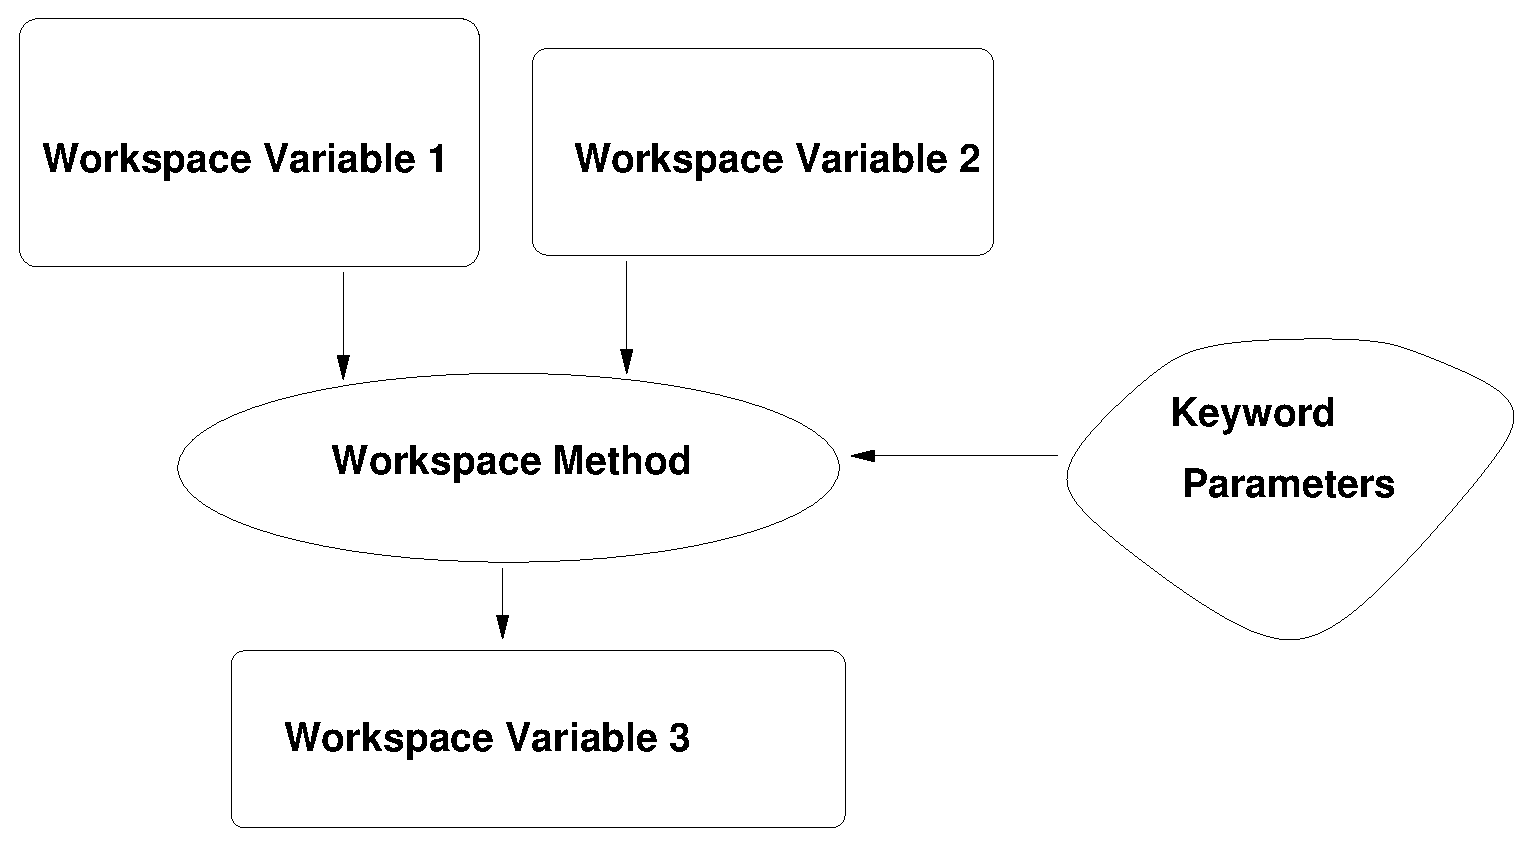
\includegraphics[width=\hsize,draft=false]{concept/method}
    \caption{\textindex{Specific
        workspace methods} act on specific workspace variables to
        generate other specific workspace variables. Additional input
        parameters can be specified as keyword parameters in the
        controlfile.}
    \label{fig:method}
  \end{center}
\end{figure}

It is important to note that the controlfile has a fixed and
well-defined syntax. This syntax is understood by the ARTS parser.
The great advantage of this concept is that it is very easy to add
new workspace variables and new workspace methods. The program has
an internal lookup table which lists all workspace methods, as well
as their input variables, output variables, and keyword
parameters. To add a new method, one just has to add an entry to
this lookup table, and write the code for the method itself. No
further changes to the program are necessary. In particular, no
changes to the program logic or to the parser. How such an extension
can be made practically is described in Section \ref{sec:development}.


\section{Generic Workspace Methods}
%=================================
\label{sec:concept:generic}

Generic methods (Figure \ref{fig:generic_method}) allow the user of
the program even more freedom than specific methods. A generic method
is for example \artsstyle{MatrixSet}, which can be used to set any
workspace variable which is a matrix. For example
\begin{quote}
  \artsstyle{MatrixSet(z\_surface){0.0}}
\end{quote}
will set all elements of \artsstyle{z\_surface} to 0.0 (as long as
\artsstyle{nrows} and \artsstyle{ncols} are set).

\begin{figure}
  \begin{center}
    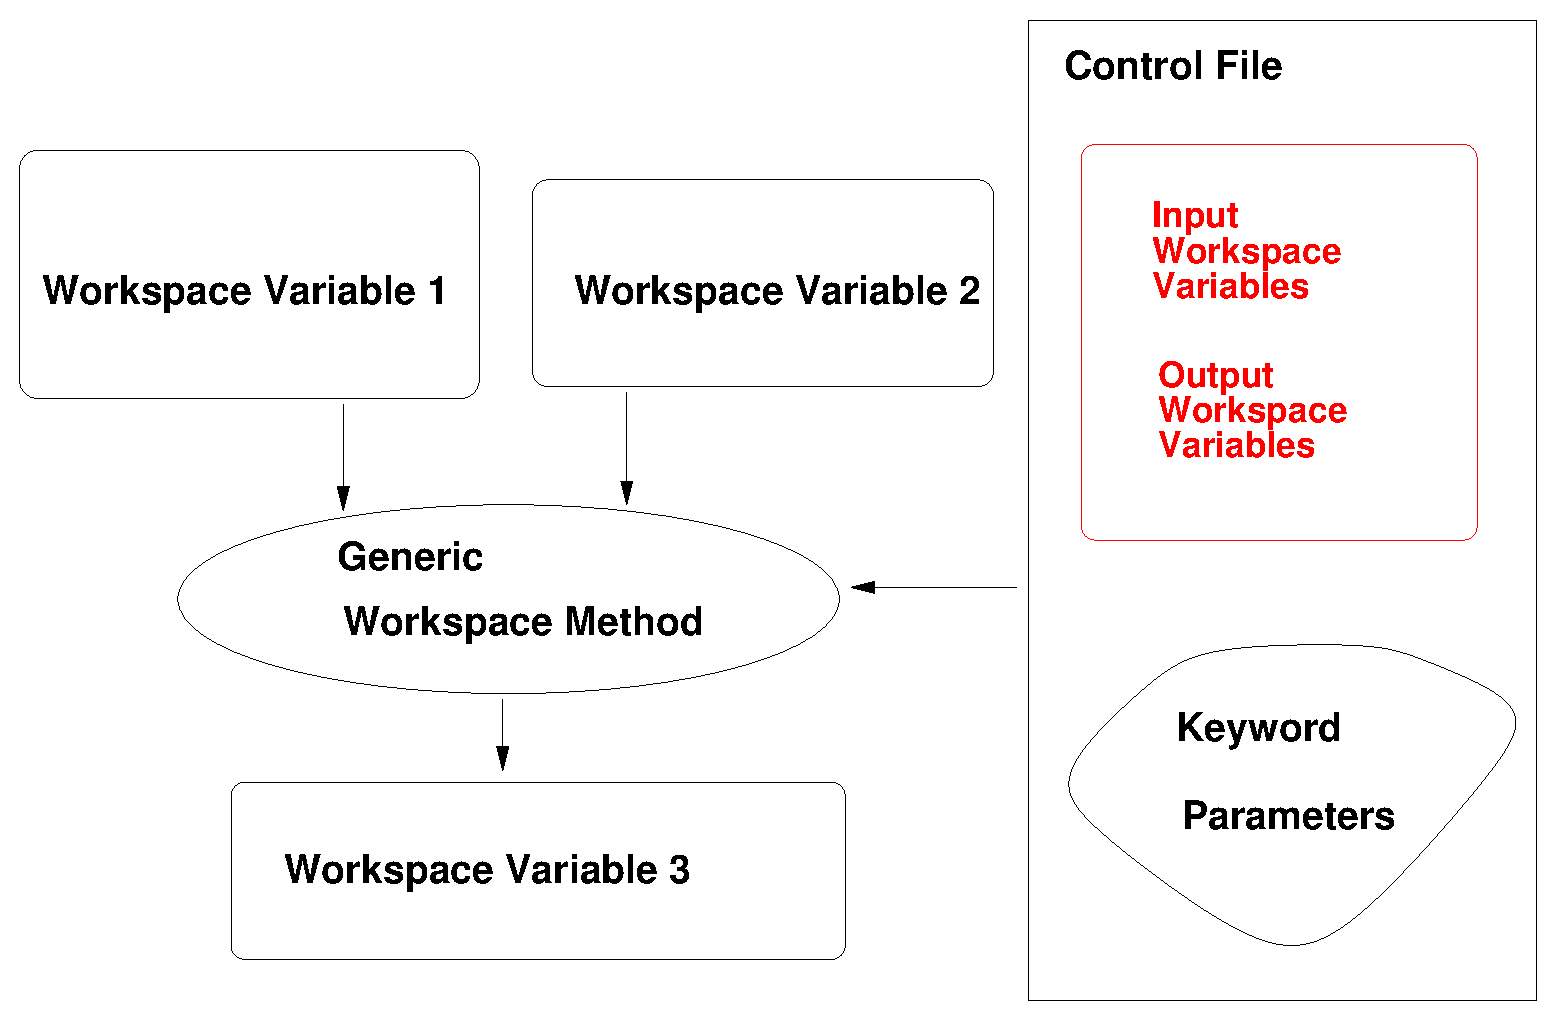
\includegraphics[width=\hsize,draft=false]{concept/generic_method}
    \caption{For \textindex{generic
      workspace methods} the workspace variables to act on are
        specified in the controlfile.}
    \label{fig:generic_method}
  \end{center}
\end{figure}

Some methods are even more flexible, the are super generic. This means
that they can take any workspace variable as input. The most commonly
used such methods are the XML file methods. A workspace variable is
read from a file in this way
\begin{quote}
  \artsstyle{ReadXML(f\_grid)\{"frequency\_grid"\}}
\end{quote}
Generic methods are particularly useful for IO operations like in the
example above. No new IO methods are necessary for new workspace
variables, as long as they are of standard types already known to the
program (for example vectors or matrices). 



\section{Agendas}
%=================================
\label{sec:concept:agendas}

Agendas are a special incarnation of a workspace method. In the
controlfile an arbitrary number of workspace methods can be added to
an agenda. On invocation, the agenda executes its methods one
after the other. The inputs and outputs defined for the agenda must
be satisfied by the invoked workspace methods. E.g., if an agenda
has \artsstyle{f\_grid} in its list of output workspace variables, a
workspace method which generates \artsstyle{f\_grid} must be added to
the agenda in the controlfile.

Even though it is possible to execute agendas directly from the
controlfile with the \artsstyle{AgendaExecute} method, the more common
and intended use case is the internal invocation by other workspace
methods. This adds a grave amount of flexibility to arts. The
\artsstyle{RteStd} method for example calculates (besides other
components) the emission term. Without the means of an agenda, it
would only be possible to use always the same method for the emission
calculation. By the use of an agenda the user can choose between
different methods to calculate the emission and plug them into the
emission agenda in the control file:

{\small
\begin{verbatim}
AgendaSet(emission_agenda){
  emissionPlanck{}
}
\end{verbatim}
}

\noindent
\artsstyle{RteStd} internally calls the \artsstyle{emission\_agenda} and
uses the user selected method for calculating the emission term.



\section{Practical hints}
%=================================
\label{sec:concept:practical}

The subdirectory \fileindex{tests} contains some example controlfiles.
You should study them to learn more about how the program works. You
can also run these controlfiles like this:
\begin{quote}
\begin{verbatim}
  arts simpleMC.arts
\end{verbatim}
\end{quote}
This assumes that you are inside the directory where the controlfiles
are, and that the \artsstyle{arts} executable is in your path.  You can
also run all of the examples, by saying
\begin{quote}
\begin{verbatim}
  make check
\end{verbatim}
\end{quote}

ARTS offers a number of useful command line parameters. In general,
there is a short form and a long form for each parameter. The short
form consists of a minus sign and a single letter, whereas the long
form consists of two minus signs and a descriptive name. To get a full
list, type
\begin{quote}
\begin{verbatim}
  arts -h
\end{verbatim}
\end{quote}
or
\begin{quote}
\begin{verbatim}
  arts --help
\end{verbatim}
\end{quote}
Most useful at the beginning should be the \artsstyle{-d}
(\artsstyle{--describe}), \artsstyle{-m} (\artsstyle{--methods}), \artsstyle{-w}
(\artsstyle{--workspacevariables}), and \artsstyle{-i} (\artsstyle{--input}) flags.
For instance, the \artsstyle{-d} (\artsstyle{--describe}) flag gives you online
documentation for any workspace method or workspace variable. Usage:
\begin{quote}
\begin{verbatim}
  arts -d f_grid
\end{verbatim}
\end{quote}
will print documentation about the workspace variable \artsstyle{f\_grid}, which
happens to be the monochromatic frequency grid.

But what methods and variables are available? You can find out by
typing
\begin{quote}
\begin{verbatim}
  arts -m all
\end{verbatim}
\end{quote}
which will list all workspace methods, or by typing 
\begin{quote}
\begin{verbatim}
  arts -w all
\end{verbatim}
\end{quote}
which will list all workspace variables. As you can see, these lists
are quite long. But you can get more specific information:
\begin{quote}
\begin{verbatim}
  arts -m f_grid
\end{verbatim}
\end{quote}
will give you a list of all methods that can generate the workspace
variable \artsstyle{f\_grid}. Specific and generic methods are listed
separately. Generic methods are in this case all methods producing a
Vector, since \artsstyle{f\_grid} belongs to this group. A similar task is
performed by the \artsstyle{-i} (\artsstyle{--input}) flag, with the difference
that \artsstyle{arts -i f\_grid} will list those methods that require
\artsstyle{f\_grid} as \emph{input}, whereas \artsstyle{arts -m f\_grid} lists
those that produce \artsstyle{f\_grid} as output. Finally,
\begin{quote}
\begin{verbatim}
  arts -w surfaceFlat
\end{verbatim}
\end{quote}
will give you all variables required by the method \artsstyle{abs\_coefCalc}
(the variable \artsstyle{f\_grid} happens to be one of them).

Using these command line parameters, it is easy to build up a
controlfile. The trick is, to start at the end. Say you want to
compute absorption coefficients. First of all, you have to find out
in which workspace variable these are stored. Look at the list
produced by \artsstyle{arts -w all}. You can use \artsstyle{arts -d} to look at
some candidates a bit more closely. This way, you will find out that
\artsstyle{abs\_coef} is the variable you are looking for.

In the next step, you can use \artsstyle{arts -m abs\_coef} to find all methods
that can calculate \artsstyle{abs\_coef}. So, you will find the method
\artsstyle{abs\_coefCalc}. Now you can use \artsstyle{arts -w abs\_coefCalc} to find out the
required input variables of that method. Then you can use the
\artsstyle{-m} flag again, to find the methods producing these variables,
and so on.

%%% Local Variables: 
%%% mode: latex
%%% TeX-master: "uguide"
%%% End: 

\part{Algorithm Descriptions}
%
% To start the document, use
%  \levela{...}
% For lover level, sections use
%  \levelb{...}
%  \levelc{...}
%
\levela{Theoretical formalism}
 \label{sec:formalism}

%
% Document history, format:
%  \starthistory
%    date1 & text .... \\
%    date2 & text .... \\
%    ....
%  \stophistory
%
\starthistory
  000306 & Written by Patrick Eriksson, partly 
           based on \citet{eriksson:99} and \citet{eriksson:00a}. \\
\stophistory



%
% Symbol table, format:
%  \startsymbols
%    ... & \verb|...| & text ... \\
%    ... & \verb|...| & text ... \\
%    ....
%  \stopsymbols
%
%
%\startsymbols
%  \mpbi   & \verb|y|      & monochromatic pencil beam intensity      \\
%  \f      & \verb|f_mono| & monochromatic frequency                  \\
%  \view   & \verb|za_pencil| & pencil beam zenith angle              \\
%  \iv     & \verb|y|      & vector of monochromatic pencil beam intensities \\
%  \y      & \verb|y|      & spectrum recorded by a sensor            \\
%  \fm     & \verb|-|      & forward model                            \\
%  \fma    & \verb|-|      & atmospheric part of \fm                  \\
%  \fms    & \verb|-|      & sensor part of \fm                       \\
%  \xt     & \verb|-|      & state vector (variables to be retrieved) \\
%  $\xt_r$ & \verb|-|      & atmospheric part of \xt                  \\
%  $\xt_s$ & \verb|-|      & sensor part of \xt                       \\
%  $\xt_\merr$& \verb|-|   & part of \xt\ describing measurement errors   \\
%  \bt     & \verb|-|      & forward model parameter vector           \\
%  $\bt_r$ & \verb|-|      & atmospheric part of \bt                  \\
%  $\bt_s$ & \verb|-|      & sensor part of \bt                       \\
%  $\bt_\merr$& \verb|-|   & part of \bt\ describing measurement errors   \\
%  \Kx     & \verb|k|      & state weighting function matrix          \\
%  \Kb     & \verb|k|      & model parameter weighting function matrix\\  
% \label{symtable:formalism}     
%\stopsymbols



%
% Introduction
%
In this section a theoretical framework for the forward model is
presented. The presentation follows \citet{rodgers:90}, but some
extensions are made, for example, the distinction between the
atmospheric and sensor parts of the forward model is also discussed
here.



\levelb{The forward model}
 \label{sec:formalism:fm}
 
 The radiative intensity, \mpbi, at a point in the atmosphere, $r$, for
 frequency \f\ and traversing in the direction, \view, is dependent
 on a variety of physical processes and continuous variables such as
 the temperature profile, $T$:

 \begin{equation}
   \mpbi = F(r,\f,\view,T,\dots)
 \end{equation} 
 To detect the spectral radiation some kind of sensor, having a finite
 spatial and frequency resolution, is needed, and the observed
 spectrum becomes a vector, \y, instead of a continuous function.
 The atmospheric radiative transfer is simulated by a computer model
 using a limited number of parameters as input, and the forward model,
 \fm, used in practice can be expressed as
 
 \begin{equation}
   \y = \fm(\xt_\fm,\bt_\fm) + \merr(\xt_\merr,\bt_\merr)
  \label{eq:formalism:fm}
 \end{equation}
 where $(\xt_\fm,\bt_\fm)$ and $(\xt_\merr,\bt_\merr)$ together give a
 total description of both the atmospheric and sensor states, and
 \merr\ is the measurement errors. The parameters are divided in such
 way that \xt, the state vector, contains the parameters to be
 retrieved, and the remainder is given by \bt, the model parameter
 vector. The total state vector is
 \begin{equation}
   \xt = \left[ \begin{array}{c} \xt_\fm \\ \xt_\merr \end{array} \right]
 \end{equation}
 and the total model parameter vector is
 \begin{equation}
   \bt = \left[ \begin{array}{c} \bt_\fm \\ \bt_\merr \end{array} \right]
 \end{equation}
 The actual forward model consists of either empirically determined
 relationships, or numerical counterparts of the physical
 relationships needed to describe the radiative transfer and sensor
 effects. The forward model described here is mainly of the latter
 type, but some parts are more based on empirical investigations, such
 as the parameterisations of continuum absorption. It should be noted
 that a possible data reduction is also part of the forward model.
  
 Both for the theoretical formalism and the practical implementation,
 it is suitable to make a separation of the forward model into two
 main sections, a first part describing the atmospheric radiative
 transfer for pencil beam (infinite spatial resolution) monochromatic
 (infinite frequency resolution) signals \citep{eriksson:99},

 \begin{equation}
   \iv = \fma(\xt_r,\bt_r)
  \label{eq:formalism:fma}
 \end{equation}
 and a second part modelling sensor characteristics,
 \begin{equation}
   \y = \fms(\iv,\xt_s,\bt_s) + \merr(\xt_\merr,\bt_\merr)
  \label{eq:formalism:fms}
 \end{equation}
 where \iv\ is the vector holding the spectral values for the
 considered set of frequencies and viewing angles (i.e.
 $\iv^i=I(\f^i,\view^i)$, where $i$ is the vector index), and
 $\xt_\fm$ and $\bt_\fm$ are separated correspondingly, that is,
 $\xt_\fm^T= [\xt_r^T,\xt_s^T]$ and $\bt_\fm^T= [\bt_r^T,\bt_s^T]$. The
 vectors \xt\ and \bt\ can now be expressed as
 \begin{equation}
   \xt = \left[ \begin{array}{c} \xt_r\\ \xt_s \\ \xt_\merr \end{array} \right]
 \end{equation}
 and
 \begin{equation}
   \bt = \left[ \begin{array}{c} \bt_r\\ \bt_s \\ \bt_\merr \end{array}\right],
 \end{equation}
 respectively.

 The subscripts of \xt\ and \bt\ are below omitted if the part of the
 vectors used is made clear by the context. 



\levelb{The sensor transfer matrix} 
 \label{sec:formalism:sensor}
  
 The modelling of the different sensor parts can be described by a
 number of of analytical expressions (see \citet{eriksson:97a}) that
 together makes the basis for the sensor model. These expressions are
 throughout linear operations and it possible, as suggested in
 \citet{eriksson:00a}, to implement the sensor model as a
 straightforward matrix multiplication:
 \begin{equation}
   \y = \Hm \iv + \merr
  \label{eq:formalism:H}
 \end{equation}
 where \Hm\ is here denoted as the sensor transfer matrix.  The matrix
 \Hm\ can  be set up to incorporate effects of a data reduction and
 the total transfer matrix is then
 \begin{equation}
   \Hm = \Hd \Hs
  \label{eq:formalism:Hs}
 \end{equation}
 as
 \begin{equation}
   \y = \Hd \y' = \Hd (\Hs \iv + \merr') = \Hm \iv + \merr
  \label{eq:formalism:datared}
 \end{equation}
 where \Hd\ is the reduction matrix, \Hs\ the sensor matrix, and $\y'$
 and $\merr'$ are the measurement vector and the measurement errors,
 respectively, before data reduction. The matrices \Hd\ and \Hs\ are
 described in Section \ref{sec:sensor} and \ref{sec:red}, respectively.



\levelb{Weighting functions} 
 \label{sec:formalism:wfuns}

 \levelc{Basics} 
 A weighting function is the partial derivative of the spectrum vector
 \y\ with respect to some variable used by the forward model.  As the
 input of the forward model is divided between \xt\ or \bt, the
 weighting functions are divided correspondingly between two matrices,
 the state weighting function matrix

 \begin{equation}
   \Kx = \frac{\partial \y}{\partial \xt}
  \label{eq:formalism:kx}
 \end{equation}
 and the model parameter weighting function matrix
 \begin{equation}
   \Kb = \frac{\partial \y}{\partial \bt}
  \label{eq:formalism:kb}
 \end{equation}
 For the practical calculations of the weighting functions, it is
 important to note that the atmospheric and sensor parts can be
 seperated. For example, if \xt\ only hold atmospheric and
 spectroscopic variables, \Kx\ can be expressed as

 \begin{equation}
   \Kx = \frac{\partial \y}{\partial \iv}\frac{\partial\iv}{\partial \xt} =
    \Hm\frac{\partial\iv}{\partial \xt}
  \label{eq:formalism:kx2}
 \end{equation}
 This equation shows that the new parts needed to calculate
 atmospheric weighting functions, are functions giving $\partial\iv /
 \partial \xt$ where \xt\ can represent the vertical profile of a
 species, atmospheric temperature, spectroscopic data etc.
 
 The practical calculation of weighting functions is discussed in
 detail in Sections \ref{sec:wfuns} and \ref{sec:wfuns_sens}.


 \levelc{Transformation between vector spaces}
 
  It could be of interest to transform a weighting function matrix from
  one vector space to another. The new vector, $\xt'$, is here
  assumed to be of length $n$ $(\xt' \in \msize{n}{1})$, while the original
  vector, \xt\ is of length $p$ $(\xt \in \msize{p}{1})$.  The
  relationship between the two vector spaces is described by a
  transformation matrix $\B$:
  \begin{equation}
    \xt = \B\xt'
  \end{equation}
  where $\B \in \msize{p}{n}$. For example, if $\xt'$ is assumed to be
  piecewise linear, then the columns of $\B$ contain tenth functions,
  that is, a function that are 1 at the point of interest and decreases
  linearly down to zero at the neighbouring points.  The matrix can
  also hold a reduced set of eigenvectors.
    
  The weighting function matrix corresponding to $\xt'$ is
  \begin{equation}
    \K_{\xt'} = \frac{\partial \y}{\partial \xt'}
  \end{equation}
  This matrix is related to the weighting function matrix of \xt\ (Eq.
  \ref{eq:formalism:kx}) as
  \begin{equation}
    \K_{\xt'}
      = \frac{\partial \y}{\partial \xt} \frac{\partial \xt}{\partial \xt'}
      = \frac{\partial \y}{\partial \xt} \B 
      = \Kx \B
  \end{equation}
  Note that
  \begin{equation}
    \K_{\xt'}\xt' = \Kx\B\xt' =  \Kx\xt
  \end{equation}
  However, it should be noted that this relationship only holds for
  those \xt\ that can be represented perfectly by some $\xt'$ (or vice
  versa), that is, $\xt=\B\xt'$, and not for all combinations of \xt\ 
  and $\xt'$.

  If $\xt'$ is the vector to be retrieved, we have that \citep{rodgers:90}
  \begin{equation}
    \xret' = \im(\y,\ct) = \tm(\xt,\bt,\ct)
  \end{equation}
  where \im\ and \tm\ are the inverse and transfer model, respectively.

  The contribution function matrix is accordingly
  \begin{equation}
    \Dy =  \frac{\partial \xret'}{\partial \y}
  \end{equation}
  that is, \Dy\ corresponds to $\K_{\xt'}$, not \Kx.
  
  We have now two possible averaging kernel matrices
  \begin{equation}
    \A_{\xt} 
      = \frac{\partial \xret'}{\partial \xt} 
      = \frac{\partial \xret'}{\partial \y} \frac{\partial \y}{\partial \xt}
      = \Dy \Kx
  \end{equation}
  \begin{equation}
    \A_{\xt'} 
      = \frac{\partial \xret'}{\partial \xt'} 
      = \frac{\partial\xret'}{\partial\y}\frac{\partial\y}{\partial\xt}
      \frac{\partial\xt}{\partial\xt'}
      = \Dy \K_{\xt'}
      = \A_{\xt} \B
  \end{equation}
  where $\A_{\xt} \in \msize{p}{n}$ and $\A_{\xt'} \in
  \msize{p}{p}$, that is, only $\A_{\xt'}$ is square. 




%%% Local Variables: 
%%% mode: latex
%%% TeX-master: "uguide"
%%% End: 

%
% To start the document, use
%  \levela{...}
% For lover level, sections use
%  \levelb{...}
%  \levelc{...}
%
\levela{Gas Absorption}
 \label{sec:absorption}


%
% Document history, format:
%  \starthistory
%    date1 & text .... \\
%    date2 & text .... \\
%    ....
%  \stophistory
%
\starthistory
  2001-07-05 & Template created by Stefan Buehler.\\
\stophistory


%
% Symbol table, format:
%  \startsymbols
%    ... & \verb|...| & text ... \\
%    ... & \verb|...| & text ... \\
%    ....
%  \stopsymbols
%
%
%\startsymbols
%  -- & -- & -- \\
% \label{symtable:wfuns}     
%\stopsymbols


Some general introduction here, also explaining the structure of this chapter.



\levelb{Line Absorption}
%-----------------------
\label{sec:line_absorption}

Some introduction here, how line by line absorption is calculated in
principle. (Should define intensity, partition function, line shape, etc.)

\levelc{Line Catalogues} 

Mostly describe the ARTS internal format, but also briefly list the
other catalogues that can be read by ARTS

\levelc{Species specific data} 

Molecular mass, etc. 

\levelc{Partition Functions}

These are strictly also species specific data, but they seem to deserve
their own section.

\levelc{Line Shape Functions}


\levelc{ARTS Workspace Variables and Methods}



\levelb{Continua and Complete Absorption Models}
%-----------------------------------------------

There should be some general introduction here.

The headings here are tentative, TBD by Thomas.

\levelc{H2O Models}

\levelc{Dry air Models}

\levelc{ARTS Workspace Variables and Methods}


 



%%% Local Variables: 
%%% mode: latex 
%%% TeX-master: "uguide" 
%%% End:


\chapter{Overview of clear-sky radiative transfer 
calculations}
 \label{sec:rte}


 \starthistory
 110611 & Extended and general revision (Patrick Eriksson).\\
 050613 & First complete version by Patrick Eriksson.\\
 \stophistory

\graphicspath{{Figs/rte/}}

This section gives an overview of the variables and the approach used to handle
radiative transfer calculations. This includes an overview of how effects
caused by the sensor and surface are incorporated. The default assumption is
that there is no particle scattering and the (atmospheric) absorption/emission
is unpolarised. This is for simplicity denoted as clear-sky calculations. Cases
involving scattering or polarised absorption are handled by the ``cloud box''
(Sec.~\ref{sec:fm_defs:cloudbox}). In short, the more demanding calculations
are restricted to a smaller domain of the model atmosphere, and the radiative
transfer in this domain is treated by dedicated workspace methods.

The section deals with general aspects of radiative transfer and the
algorithms applied outside the cloud box. Even though the atmospheric absorption
and emission outside the cloud box are unpolarised, the expressions to apply
must allow that polarisation signals from the surface and the cloud box are
correctly propagated to the sensor.




\section{Stokes dimensionality}
%==============================================================================
\label{sec:fm_defs:polarisation}

To full polarisation state of radiation can be described by the Stokes
vector. The vector can be defined in different ways, but it has always
four elements. The Stokes vector, \StoVec, is here written as
\begin{equation}
  \label{eq:fm_defs:stokevec}
  \StoVec = \left[
  \begin{array}{c}
   I\\Q\\U\\V
  \end{array}
  \right],
\end{equation}
where the first component ($I$) is the full intensity of the
radiation, the second component ($Q$) is the difference between
vertical and horizontal polarisation, the third component ($U$) is the
difference for $\pm$45$^\circ$ polarisation and the last component
($V$) is the difference between left and right circular polarisation.
That is:
\begin{eqnarray}
  I &=&   \Iv + \Ih = \Ipff + \Imff = \Ilhc + \Irhc, \\
  Q &=&   \Iv - \Ih,                                 \\
  U &=&   \Ipff - \Imff,                             \\
  V &=&   \Ilhc - \Irhc,                             
\end{eqnarray}
where \Iv, \Ih, \Ipff, and \Imff\ are the intensity of the component linearly
polarised at the vertical, horizontal, +45\degree\ and -45\degree\ direction,
respectively, and \Irhc, and \Ilhc\ are the intensity for the right- and
left-hand circular components. Further details on polarisation and the
definition of the Stokes vector are found in \theory,
Section~\ref{T-sec:polarization}.

ARTS is a fully polarised forward model, but can be run with a smaller
number of Stokes components. The selection is made with the workspace
variable \wsvindex{stokes\_dim}. For example, gaseous absorption and
emission are in general unpolarised, and if not scattering has to be
considered it is sufficient to only include the first Stokes
components in the simulations. To include higher order Stokes
components results only, in this case, in slower calculations. The
general case is here denoted as \textindex{vector radiative transfer},
while \textindex{scalar radiative transfer} refers to the case when
only the first Stokes component is considered.
 



\section{Overall calculation procedure}
%===================
\label{sec:fm_defs:calcproc}

The structure of the part handling complete radiative transfer calculations is
fixed, where the main workspace method is denoted as \wsmindex{yCalc}. That is,
most ARTS control files include a call of \artsstyle{yCalc} and this section
outlines this method and the associated main variables.

The calculation approach fits with the formalism presented in Sections
\ref{T-sec:formalism:fm}-\ref{T-sec:formalism:sensor} of \theory, where the
separation between atmospheric radiative transfer and inclusion of sensor
effects shall be noted especially, and a similar nomenclature is used here:
\begin{description}
\item[\MsrVct]: Complete measurement vector. In addition to atmospheric
  radiative transfer, the vector can include effects by sensor characteristics
  and data reduction operations. The corresponding workspace variable is 
  \wsvindex{y}.
\item[\aMpiVct{b}]: Monochromatic pencil beam data for a measurement block. The
  definition of a measurement block is found in
  Section~\ref{sec:fm_defs:seqsandblocks}. This vector is only affected by
  atmospheric radiative transfer. Only used internally and there is no
  corresponding workspace variable.
\item[\aMpiVct{y}]: Monochromatic data for a single (pencil beam)
  line-of-sight. \aMpiVct{b} consists of one or several \aMpiVct{y} appended.
  The corresponding workspace variable is \wsvindex{iy}.
\item[\aSnsMtr{b}]: The complete sensor response matrix, for a measurement
  block. Can include data reduction. The corresponding workspace variable is
  \wsvindex{sensor\_response}.
\end{description}
The \artsstyle{yCalc} method is outlined in Algorithm~\ref{alg:fm_defs:yCalc}.
For further details of each calculation step, see the indicated equation or
section. In summary, \artsstyle{yCalc} appends data from different pencil beam
calculations and applies the sensor response matrix (\aSnsMtr{b}). The actual
radiative transfer calculations are not part of \artsstyle{yCalc}, but are
performed by \artsstyle{iy\_clearsky\_agenda}
(Algorithm~\ref{alg:fm_defs:iyCSagenda}). This agenda, in its turn, makes us of
other agendas, such as \artsstyle{ppath\_step\_agenda}.
\begin{algorithm}
 \begin{algorithmic}
  \STATE{allocate memory for the matrix $\MsrVct$}
  \COMMENT{Equation \ref{eq:fm_defs:measseq}}
  \STATE{allocate memory for the matrix \aMpiVct{b}}
  \COMMENT{Equation \ref{eq:fm_defs:freqs_of_ib}}
  \FORALL{sensor positions}
   \FORALL[Section \ref{sec:fm_defs:seqsandblocks}]
                                    {pencil beam directions of the block}
    \STATE{call \artsstyle{iy\_clearsky\_agenda}, giving \aMpiVct{y}}
    \COMMENT{Algorithm \ref{alg:fm_defs:iyCSagenda}}
    \STATE{unit conversion of \aMpiVct{y} following \wsvindex{y\_unit}}
    \COMMENT{Section \ref{sec:fm_defs:unit}}
    \STATE{copy \aMpiVct{y} to correct part of \aMpiVct{b}}
   \ENDFOR
   \STATE{put the product \aSnsMtr{b}\aMpiVct{b} in correct part of 
          $\MsrVct$}
  \ENDFOR
 \end{algorithmic}
 \caption{Outline of the overall clear sky radiative transfer calculations
   (\artsstyle{yCalc}).}
 \label{alg:fm_defs:yCalc}
\end{algorithm}

\begin{algorithm}
 \begin{algorithmic}
   \STATE{determine the propagation path by \artsstyle{ppath\_calc}}
   \COMMENT{Section \ref{sec:fm_defs:ppaths}}
   \STATE{determine the radiation at the start of the propagation path}
   \COMMENT{Section \ref{sec:fm_defs:rad_bkgr}}
   \STATE{perform radiative transfer along the propagation path}
   \COMMENT{Section \ref{sec:fm_defs:rte}}
 \end{algorithmic}
 \caption{The main operations for methods to be part of
   \wsvindex{iy\_clearsky\_agenda}. The same applies to methods for
   \wsvindex{iy\_clearsky\_basic\_agenda}.}
 \label{alg:fm_defs:iyCSagenda}
\end{algorithm}

That is, \artsstyle{yCalc} is a common method, independent of the details of
the radiative transfer. For exemple, \artsstyle{yCalc} is used both if emission
measurements or pure transmission data are simulated, that choice is made
inside \artsstyle{iy\_clearsky\_agenda} (see further Section
\ref{sec:fm_defs:rte}). Further, if refraction is considered or not is
controled by \artsstyle{ppath\_step\_agenda}. 

The three following sections describes the main calculation steps of 
\artsstyle{iy\_clearsky\_agenda}, in the order they are exucuted.


\section{Propagation paths}
%===================
\label{sec:fm_defs:ppaths}

A pencil beam path through the atmosphere to reach a position along a
specific line-of-sight is denoted as the \textindex{propagation path}.
Propagation paths are described by a set of points on the path, and
the distance along the path between the points. These quantities, and
a number of auxiliary variables, are stored together in a structure
described in Section~\ref{sec:ppath:Ppath}. The path points are
primarily placed at the crossings of the path with the atmospheric
grids (\artsstyle{p\_grid}, \artsstyle{lat\_grid} and
\artsstyle{lon\_grid}). A path point is also placed at the sensor if
it is placed inside the atmosphere.  Points of surface reflections and
tangent points are also included if such exist. More points can also
be added to the propagation path, for example, by setting an upper
limit for the distance along the path between the points.

\begin{figure}
 \begin{center}
  \includegraphics*[width=0.95\hsize]{ppath_cases2}
  \caption{Examples on allowed propagation paths for a 2D atmosphere. 
    The atmosphere is plotted as in Figure~\ref{fig:fm_defs:2d} beside
    that the points for the atmospheric fields are not emphasised.
    The position of the sensor is indicated by an asterix $(\ast)$,
    the points defining the paths are plotted as circles $(\circ)$,
    joined by a solid line. The part of the path outside the
    atmosphere, not included in the path structure, is shown by a
    dashed line. Path points corresponding to a tangent point are
    marked by an extra plus sign $(\oplus)$. The shown paths include
    the minimum set of definition points. There exists also the
    possibility to add points inside the grid cells, for example, to
    ensure that the distance between the path points does not exceed
    a specified limit.}
  \label{fig:fm_defs:ppath_cases2}
 \end{center}
\end{figure}
% This figure was produced by the Matlab function mkfigs_ppath_cases.

\begin{figure}
 \begin{center}
  \includegraphics*[width=0.95\hsize]{ppath_cases1}
  \caption{Examples on allowed propagation paths for a 1D atmosphere
    with an activated cloud box. Plotting symbols as in
    Figure~\ref{fig:fm_defs:ppath_cases2}. When the sensor is placed 
    inside the cloud box, the path is defined with a single point, 
    to know for which position and line-of-sight the intensity field of
    the cloud box shall be interpolated. }
  \label{fig:fm_defs:ppath_cases1}
 \end{center}
\end{figure}
% This figure was produced by the Matlab function mkfigs_ppath_cases.

\begin{figure}
 \begin{center}
  \includegraphics*[width=0.95\hsize]{ppath_badcases}
  \caption{Examples on \emph{not} allowed propagation paths for a 2D 
    atmosphere. The constraints for allowed paths are discussed in the
    text.}
  \label{fig:fm_defs:ppath_badcases}
 \end{center}
\end{figure}
% This figure was produced by the Matlab function mkfigs_ppath_cases.


The propagation paths are determined basically by starting at the
sensor and following the path backwards by some \textindex{ray
  tracing} technique. If the sensor is placed above the model
atmosphere, geometrical calculations are used (as there is no
refraction in space) to find the crossing between the path and the top
of the atmosphere where the ray tracing then starts. Paths are tracked
backwards until the top of the atmosphere is reached, or there is an
intersection with the cloud box or the surface. The propagation path
(or paths) before a surface reflection is calculated when determining
the up-welling radiation from the surface
(Section~\ref{sec:fm_defs:surface}). Example on propagation
paths are shown in Figures~\ref{fig:fm_defs:ppath_cases2} and 
\ref{fig:fm_defs:ppath_cases1}.
 
Not all propagation paths are allowed for 2D and 3D. The paths can
only enter and leave the model atmosphere at the top of the
atmosphere, as the atmospheric fields are treated to be undefined
outside the covered latitude and longitude ranges
(Figure~\ref{fig:fm_defs:ppath_badcases}). In addition, if the sensor
is placed outside the model atmosphere, the line-of-sight zenith angle
must be $\geq90\degree$, and the tangent point position of the
propagation paths must be inside the end points of the latitude and
longitude grids, but can be above the top of the atmosphere. Hence, it
is allowed that the propagation path is totally outside the
atmosphere, as long as the viewing direction is downward and the
lowest point of the path, the tangent point, is inside the latitude
and longitude limits of the model atmosphere.

Propagation paths can be calculated seperately by the method
\wsmindex{ppathCalc}. However, for standard calculations the propagation paths
are calculated internally by \artsstyle{yCalc}. The calculation of the path
from one crossing of the grids to next crossing is defined by
\wsaindex{ppath\_step\_agenda}. Depending on which function that is selected
for \artsstyle{ppath\_step\_agenda}, refraction will be considered. Available
workspace methods are presented in Section~\ref{sec:ppath:usage}.




\section{The radiative background}
%===================
\label{sec:fm_defs:rad_bkgr}

\subsection{Overview}
%===================
%
The radiative intensity at the starting point of the path, and in the
direction of the line-of-sight at that point, is denoted as the
\textindex{radiative background}. Four possible radiative backgrounds
exist:
\begin{description}
\item[Space] When the propagation path starts at the top of the
  atmosphere, space is the radiative background. The normal case
  should be to set the radiation at the top of the atmosphere to be
  cosmic background radiation. An exception is when the sensor is
  directed towards the sun. The radiative background at the top of the
  atmosphere is determined by \wsaindex{iy\_space\_agenda}. If a
  propagation path is totally outside the model atmosphere, the
  observed monochromatic pencil beam intensity (\aMpiVct{y}\ in
  Algorithm~\ref{alg:fm_defs:yCalc}) equals the output of
  \artsstyle{iy\_space\_agenda}.
\item[The surface] The sum of surface emission and radiation reflected by the
  surface is the radiative background when the propagation path intersects with
  the surface. The calculation of the up-welling radiation from the surface is
  treated by a dedicated section below (Section~\ref{sec:fm_defs:surface}.)
\item[Surface of cloud box] For cases when the propagation path enters
  the cloud box the radiative background is the intensities leaving
  the cloud box. This radiation is obtained by
  \wsaindex{iy\_cloudbox\_agenda}. 
\item[Interior of cloud box] If the sensor is situated inside the
  cloud box, there is basically no propagation path. The radiative
  background, and also the final spectrum, equals the internal
  intensity field of the cloud box at the position of the sensor, in
  the direction of the sensor line-of-sight. This case is also handled
  by \artsstyle{iy\_cloudbox\_agenda}.
\end{description}
It should be noted that except for the first case above, the determination of
the radiative background involves further radiative transfer calculations. For
example, in the case of surface reflection, the down-welling radiation is
determined by a new call of \artsstyle{iy\_clearsky\_agenda} and the radiative
background for that calculation is then space or the cloud box. The intensity
field entering the cloud box is calculated by calls of
\artsstyle{iy\_clearsky\_basic\_agenda} (with cloud box deactivated) and the
radiative background is then space or the surface. This results in that space
is normally the ultimate radiative background for the calculations. The
exception is for propagation paths that intersects with the surface, and the
surface is treated to act as a blackbody. For such cases, the propagation path
effectively starts at the surface.


\subsection{Surface scattering and emission}
%===================
\label{sec:fm_defs:surface}

If there is an interception of the propagation path by the surface,
emission and scattering by the surface must be considered. The overall
treatment of these effects is fixed. The upwelling radiation from the surface
can be written as (Figure~\ref{fig:fm_defs:surface_refl})
\begin{equation}
  \MpiVct_s^u = \MpiVct_e + \sum_l^{} \mathbf{R}_l \MpiVct_l^d
  \label{eq:fm_defs:surfacerefl}
\end{equation}
where \MpiVct\ is the Stokes vector for one frequency, $\MpiVct_s^u$
is the total upward travelling intensity from the surface along the
propagation path, $\MpiVct_e$ is the emission from the surface,
$\MpiVct_l^d$ is the downward travelling intensity reaching the
surface along direction $l$, and $\mathbf{R}_l$ is the reflection
coefficient matrix from direction $l$ to the present propagation path.
The emission from the surface $(\MpiVct_e)$ is stored in
\wsvindex{surface\_emission}, the directions $l$ for which downward
travelling intensities are given by \wsvindex{surface\_los}, and the
reflection coefficients $(\mathbf{R})$ are stored in
\wsvindex{surface\_rmatrix}. These workspace variables are handled by
\wsaindex{surface\_prop\_agenda}. Surface reflections and emission are
discussed further in Section~\ref{sec:surface}.
\begin{figure}
 \begin{center}
  \includegraphics*[width=0.95\hsize]{ground_refl}
  \caption{Schematic of Equation \ref{eq:fm_defs:surfacerefl}.}
  \label{fig:fm_defs:surface_refl}
 \end{center}
\end{figure}



\section{Basic radiative transfer variables and expressions}
%---
\label{sec:fm_defs:rte}

Atmospheric radiative transfer is solved for each individual pencil beam
direction (line-of-sight) individually. It is the task of
\wsvindex{iy\_clearsky\_agenda} to perform a single such clear sky radiative
transfer calculation. All methods developed for
\artsstyle{iy\_clearsky\_agenda} adapt automatically to the value of
\wsvindex{stokes\_dim}.

This section describes how the core radiative transfer equation is solved
practically in ARTS. Focus is put on emission measurements as ARTS is
intended primarily for such observations. However, simulations of transmission
measurements are also possible.

Beside the actual radiances, \artsstyle{iy\_clearsky\_agenda} can provide
weighting functions and auxiliary data. These later variables are not supported
by all parts of ARTS, and for efficiency reasons there exists a simpler version
of the agenda. This version is denoted as
\wsvindex{iy\_clearsky\_basic\_agenda} and returns only radiances.


\subsection{Cases with emission}
%===================
\label{sec:fm_defs:emission}

The complete vector radiative transfer equation, including scattering, is given
by Equation \ref{T-eq:rtetheory:VRTE} in \theory. If scattering can be
neglected, the equation can be written as
\begin{equation}
  \label{eq:rte:vrte}
  \frac {\DiffD\StoVec}{\DiffD s} = -\ExtMat\StoVec + \AbsVec B,
\end{equation}
where \StoVec\ is the intensity vector (the Stokes vector), $s$ is the distance
along the propagation path, \ExtMat\ is the extinction matrix, \AbsVec\ is the
absorption vector and $B$ is the source function (a scalar). If local
thermodynamic equilibrium applies, $B$ equals the Planck function describing
blackbody radiation. See further \theory, Section~\ref{T-sec:rte_theory}. For
``clear-sky conditions'' the matrix \ExtMat\ is diagonal, with all diagonal
elements equal, and only the first of the elements of \AbsVec\ is non-zero.

The radiative transfer equation above can be solved in many ways, and with
different level of refinement. The standard approach in ARTS is to solve the
radiative transfer from one point of the propagation path to next for the first
Stokes element as (compare \theory, Equation~\ref{T-eq:rtetheory:layer})
\begin{equation}
  \label{eq:fm_defs:rte_step}
  I_{i+1} = I_ie^{-\aOth{i}} + \bar{B}_i(1-e^{-\aOth{i}}),
\end{equation}
with
\begin{eqnarray}
  \bar{B}_i &=& (B(T_i)+B(T_{i+1}))/2, \\
  \aOth{i} &=& \Delta s_i(k_i+k_{i+1})/2, 
  \label{eq:taustep}
\end{eqnarray}
where $I_i$, $T_i$ and $k_i$ are the radiance, temperature and absorption
coefficient, respectively, at point $i$ of the propagation path, and $\Delta
s_i$ is the distance along the path between point $i$ and $i+1$. That is,
$\bar{B}_i$ is a Planck function average of the path step, and the absorption
is assumed to vary linearly between the two points. The start value of \Mpi\ is
determined by the radiative background (Section \ref{sec:fm_defs:rad_bkgr}).

% \begin{equation}
%   \Mpi_{i+1}(\Frq) = \Mpi_i(\Frq)e^{-\aOth{i}} + B(\Frq,\aTmp{i})(1-e^{-\aOth{i}})
%   \label{eq:fm_defs:rte_step}
% \end{equation}
% where $\Mpi(\Frq)$ is the monochromatic intensity, $i$ is path step index,
% \aOth\ is the optical thickness, $B$ the Planck function, and \Tmp\ is the
% temperature. The optical thickness of the path step, $\aOth{i}$, is calculated
% as the mean of the absorption at the end points of the step, multiplied with
% the propagation path length. The effective temperature of the path step,
% $\aTmp{i}$, is calculated likewise, as the mean of the temperature at the end
% points of the step. 

As mentioned, the emission is unpolarised for the conditions assumed here, and
the emission term vanishes for higher Stokes elements. Accordingly, the
expression for the second Stokes component is
\begin{equation}
  Q_{i+1}(\Frq) = Q_i(\Frq)e^{-\aOth{i}}.
  \label{eq:fm_defs:rte_step2}
\end{equation}
The third and forth Stokes component are handled likewise.

The expressions above are implemented in the workspace method
\wsmindex{iyEmissionStandardClearsky}, intended to be part of
\artsstyle{iy\_clearsky\_agenda}. For inclusion in
\artsstyle{iy\_clearsky\_basic\_agenda}, there is a version denoted as
\wsmindex{iyEmissionStandardClearskyBasic}


\subsection{Pure transmission calculations}
%===================
\label{sec:fm_defs:transmission}

If only the attenuation of a signal is of concern (i.e.\ atmospheric and
surface emissions are neglected), Equation~\ref{eq:fm_defs:rte_step2} can be
applied for all Stokes elements. The initiation of the Stokes vector by the
radiative background must also be adopted. Otherwise the calculations are
performed exactly as for cases with emission.

Calculations of pure transmission type are performed by the method denoted as
\wsmindex{iyBeerLambertStandardClearsky}. This method is complemented by
\wsmindex{iyBeerLambertStandardCloudbox}, to be applied inside the cloud box.


\section{Output unit}
%==============================================================================
\label{sec:fm_defs:unit}

There is no fixed unit for calculated spectra (\wsvindex{y}), it depends on the
calculation set-up. For example, if emission is considered, or if just
transmissions are calculated. 

The primary unit for emission data (radiances) is [W/(Hz$\cdot$m$^2\cdot$sr)].
The emission intensity corresponds directly with the definition of the Planck
function in \theory, Equation~\ref{T-eq:rtetheory:planck}. This radiance can be
converted to other emission units by the workspace variable \wsvindex{y\_unit}.

Expressions for the unit conversion and further details are found in
\citet{eriksson:arts2:11}.



\section{Compulsory sensor and data reduction variables}
%==============================================================================
\label{sec:fm_defs:sensor1}

The instrument that detects the simulated radiation is denoted as the
sensor\index{sensor, the}. The forward model is constructed in such
way that a sensor must exist. For cases when only monochromatic pencil
beam radiation is of interest, the positions and directions for which
the radiation shall be calculated are given by specifying an imaginary
sensor with infinite frequency and angular resolution. The workspace
variables for the sensor that always must be specified are
\artsstyle{sensor\_response}, \artsstyle{sensor\_pos},
\artsstyle{sensor\_los}, \artsstyle{antenna\_dim},
\artsstyle{mblock\_za\_grid} and \artsstyle{mblock\_aa\_grid}. These
variables are presented separately
below. 


\subsection{Sensor position\index{sensor position}}
%===================
\label{sec:fm_defs:sensorpos}

The observation positions of the sensor are stored in
\wsvindex{sensor\_pos}. This is a matrix where each row corresponds to
a sensor position. The number of columns in the matrix equals the
atmospheric dimensionality (1 column for 1D etc.). The columns of the
matrix (from first to last) are radius, latitude and longitude.
Accordingly, row $i$ of \artsstyle{sensor\_pos} for a 3D case is
$(\aRds{i},\aLat{i},\aLon{i})$. The sensor position can be set to any
value, but the resulting propagation paths (also dependent on
\artsstyle{sensor\_los}) must be valid with respect to the model
atmosphere (see Section~\ref{sec:fm_defs:ppaths}). An obviously
incorrect choice is to place the senor below the surface altitude. If
the sensor is placed inside the model atmosphere, any sensor
line-of-sight is allowed, this including the cases that the sensor is
placed on the surface looking down, and that the sensor is placed
inside the cloud box.

The fact that the sensor position can be given any value implies that
the radius must be used in \artsstyle{sensor\_pos}, in contrast to
\artsstyle{z\_surface} and \artsstyle{z\_field} where the altitude
above the geoid is applied. This is the case as, for 2D and 3D, the
sensor can be placed outside the covered latitude and longitude
ranges, thus outside the defined geoid, and the geometrical altitude is
undefined. 

The sensor is treated to be motionless when calculating the spectrum,
or spectra, for each given observation position. One or several
spectra can be calculated for each position as described in
Section~\ref{sec:fm_defs:seqsandblocks}.


\subsection{Line-of-sight\index{line-of-sight}}
%===================
\label{sec:fm_defs:los}

The viewing direction of the sensor, the line-of-sight, is described
by two angles, the zenith angle (\ZntAng) and the azimuth angle
(\AzmAng). The zenith angle exists for all atmospheric
dimensionalities, while the azimuth angle is defined only for 3D.
The term line-of-sight is not only used in connection with the sensor,
it is also used to describe the local propagation direction along the
path taken by the observed radiation
(Section~\ref{sec:fm_defs:ppaths}).  The zenith and azimuthal angles
are defined in an identical way in both of these contexts (sensor
pointing direction; local propagation direction). This is expected as
the position of the sensor is the end point of the propagation path.
The sensor line-of-sight is the direction the antenna is pointed to
receive the radiation. The line-of-sight for propagation paths is
defined likewise, it is the direction in which a hypothetical sensor
must be placed to receive the radiation along the propagation path at
the point of interest. This means that the line-of-sight and the
photons are going in opposite directions. As a true sensor has a
finite spatial resolution (described by the antenna pattern),
theoretically there is an infinite number of line-of-sights associated
with the sensor, but in the forward model, spectra are only calculated
for a discrete set of directions. If a sensor line-of-sight is
mentioned without any comments, it refers to the direction in which
the centre of the antenna pattern is directed.

\begin{figure}
 \begin{center}
  \begin{minipage}[c]{0.6\textwidth}
   \includegraphics*[width=0.99\hsize]{za_and_aa_angles}
  \end{minipage}%
  \begin{minipage}[c]{0.4\textwidth}
   \caption{Definition of zenith angle, \ZntAng, and azimuth angle, 
       \AzmAng, for a line-of-sight. The figure shows a line-of-sight
       with a negative azimuth angle.}
   \label{fig:fm_defs:los}
  \end{minipage}
 \end{center}
\end{figure}           
 
The \textindex{zenith angle}, \ZntAng, is simply the angle between the
line-of-sight and the zenith direction (Figure~\ref{fig:fm_defs:los}).
The valid range for 1D and 3D cases is $[0,180\degree]$. In the case
of 2D, zenith angles down to -180\degree\ are also allowed, where the
distinction is that positive angles mean a viewing direction towards
higher latitudes, and negative angles mean a viewing direction towards
lower latitudes. It should be mentioned that the zenith and nadir
directions are here defined to be along the line passing the centre of
the coordinate system and the point of concern
(Section~\ref{sec:ppath:geoid}). A nadir observation,
$\ZntAng=180\degree$, is thus a measurement towards the centre of the
coordinate system.

The \textindex{azimuth angle}, \AzmAng, is given with respect to the
\textindex{meridian plane}.  That is, the plane going through the
north and south poles of the coordinate system $(\Lat=\pm90\degree)$
and the sensor. The valid range is $[-180\degree,180\degree]$ where
angles are counted clockwise; 0\degree means that the viewing or
propagation direction is north-wise and +90\degree\ means that the
direction of concern goes eastward. This definition does not work for
position on the poles. To cover these special cases, the definition is
extended to say that for positions on the poles the azimuth angle
equals the longitude along the viewing direction. For example, if
standing on any of the poles and the viewing direction is towards
Greenwich, the azimuth angle is 0\degree.

The sensor line-of-sights are stored in \wsvindex{sensor\_los}. This
workspace variable is a matrix, where the first column holds zenith
angles and the second column is azimuth angles. For 1D and 2D there is
only one column in the matrix, while for 3D a row $i$ of the matrix is
$(\aZntAng{i},\aAzmAng{i})$. The number of rows for
\artsstyle{sensor\_los} must be the same as for
\artsstyle{sensor\_pos}.


\subsection{Sensor characteristics and data reduction}
%===================
\label{sec:fm_defs:sensorchar}

The term ``sensor characteristics''\index{sensor characteristics} is
used here as a comprehensive term for the response of all sensor parts
that affect how the field of monochromatic pencil beam intensities are
translated to the recorded spectrum. For example, the antenna pattern,
the side-band filtering and response of the spectrometer channels are
normally the most important characteristics for a microwave heterodyne
radiometer. Any processing of the spectral data that takes place
before the retrieval is denoted as \textindex{data reduction}. The
most common processing is to represent the original spectra with a
smaller set of values, that is, a reduction of the data size. The most
common data reduction techniques is binning and Hotelling
transformation by an eigenvector expansion.

In ARTS, the influence of sensor characteristics and data reduction is
incorporated by transfer matrices\index{sensor transfer matrix}. The
application of these transfer matrices assumes that each step is a
linear operation, which should be the case for the response of the
parts of a well designed instrument. Non-linear data reduction could
be handled by special workspace methods.

The sensor and data reduction are described as a series of units, each
having its own transfer matrix.  There is only one compulsory transfer
matrix and it is \wsvindex{sensor\_response}. There are several workspace
variables associated with this transfer matrix where
\wsvindex{antenna\_dim}, \wsvindex{mblock\_za\_grid} and
\wsvindex{mblock\_aa\_grid} are the compulsory ones.

The variable \artsstyle{antenna\_dim} gives the dimensionality of the
antenna pattern\index{antenna pattern dimensionality}, where the
options are 1 and 2, standing for 1D and 2D, respectively. A 1D
antenna dimensionality means that the azimuth extension of the
antenna pattern is neglected, there is only a zenith angle variation
of the response. A 2D antenna pattern is converted to a 1D pattern by
integrating the azimuth response for each zenith angle. For cases
with 1D antenna patterns, \artsstyle{mblock\_aa\_grid} must be set to
be an empty vector.

For each sensor position, a number of monochromatic pencil beam
spectra are calculated. The monochromatic frequencies are given by
\artsstyle{f\_grid}. The pencil
beam directions are obtained by summing the sensor line-of-sight
angles (\artsstyle{sensor\_los}) for the position and the values of
\artsstyle{mblock\_za\_grid} and \artsstyle{mblock\_aa\_grid}. For
example, pencil beam zenith angle $i$ is calculated as
\begin{equation}
  \aZntAng{i} = \aZntAng{0} + \Delta\aZntAng{i}
  \label{eq:fm_defs:psi_grid}
\end{equation}
where \aZntAng{0} is the sensor line-of-sight for the position of
concern and $\Delta\aZntAng{i}$ is value $i$ of
\artsstyle{mblock\_za\_grid}.  With other words,
\artsstyle{mblock\_za\_grid} and \artsstyle{mblock\_aa\_grid} give
the grid (relative to the sensor line-of-sight) for the calculation of
the intensity field that will be weighted with the antenna response.


\subsection{Measurement sequences and blocks}
%===================
\label{sec:fm_defs:seqsandblocks}

The series of observations modelled by the simulations is denoted as
the \textindex{measurement sequence}. That is, a measurement sequence
covers all spectra recorded at all considered sensor positions. A
measurement sequence consists of one or several \textindex{measurement
  block}s. The observations inside the various blocks differ only with
an off-set of the line-of-sight, all other factors should be common
for all blocks. A block can be treated as a measurement cycle that is
repeated, an integer number of times, to form the measurement
sequence.  The measurement blocks correspond normally to each unique
sensor position of the sequence.

A measurement block covers one or several recorded spectra, depending
on the measurement conditions and the atmospheric dimensionality. A
block can consist of several spectra when there is no effective motion
of the sensor with respect to the atmospheric fields. It should be
noted that for 1D cases, a motion along a constant radius has no
influence on the simulated spectra as the same atmospheric fields are
seen for a given viewing direction. It is favourable, if possible, to
handle all spectra as a single block, instead of using a block for
each sensor position. This is the case as the antenna patterns for the
different line-of-sights are normally overlapping and a pencil beam
spectrum can be used in connection with several measurement spectra to
estimate the intensity field. If a measurement sequence is divided
into several blocks even if a single block would be sufficient, pencil
beam spectra for basically identical propagation paths can be
calculated several times, which of course will increase the
computational time. To summarise, for cases when the sensor is not in
motion, or with a 1D atmosphere and a sensor not moving vertically,
the aim should be to use a single block for the measurement sequence.

If not a single block is used, the standard option should be that the
blocks cover one spectrum each. There could exist reasons to select an
intermediate solution, to let the extent of the blocks be several
spectra (but not the full measurement sequence). This could be the
case when the atmospheric dimensionality is 2D or 3D, and the sensor
is moving but the movement during some subsequent spectra can be
neglected. If this can be done must be judged by comparing the
movement of the sensor during the extent of the considered block size
and the spatial resolution, in the direction of the movement, that is
hoped to be achieved. If this intermediate solution shall be an
option, the difference in zenith and azimuth angles between the
spectra must be the same for all blocks, otherwise
\artsstyle{sensor\_response} cannot be applied for all blocks as done
below in Equation~\ref{eq:fm_defs:measseq}.

For each block, pencil beam spectra are calculated for the
line-of-sights obtained when summing \wsvindex{sensor\_los} and
\wsvindex{mblock\_za\_grid} (and possibly
\wsvindex{mblock\_aa\_grid}), as described in
Section~\ref{sec:fm_defs:sensorchar}. The pencil beam spectra for each
line-of-sight are appended vertically to form a common vector,
\aMpiVct{b}. Values are put in following the order in
\artsstyle{f\_grid}. Hence, the frequencies for this vector are
\begin{equation}
  \aMpiVct{b} = 
  \left[ \begin{array}{c} 
     \left[
          \begin{array}{c} \aFrq{1}\\\vdots\\\aFrq{n} \end{array} 
     \right] \\
     \vdots \\
     \left[
          \begin{array}{c} \aFrq{1}\\\vdots\\\aFrq{n} \end{array} 
     \right]
     \end{array} \right]
  \label{eq:fm_defs:freqs_of_ib}
\end{equation}
where \aFrq{i} is element $i$ of \artsstyle{f\_grid} and $n$ the length of
the same vector. The order of the angles inside \artsstyle{mblock\_za\_grid}
and \artsstyle{mblock\_aa\_grid} is followed when looping the pencil beam
directions, where the azimuth angle direction is the innermost loop.
That is, for 2D antenna patterns all azimuth angles are looped for the
first zenith angle etc. 

The workspace variable \artsstyle{sensor\_response} is here denoted as
\aSnsMtr{b}. It is applied on each \aMpiVct{b} and the results are
appended vertically, following the order of the positions in
\artsstyle{sensor\_pos}
\begin{equation}
  \MsrVct = \left[ \begin{array}{c} \aSnsMtr{b}\aMpiVct{{b,1}} \\ 
                                    \aSnsMtr{b}\aMpiVct{{b,2}} \\
                                    \vdots                     \\
                                    \aSnsMtr{b}\aMpiVct{{b,n}} 
            \end{array} \right]
  \label{eq:fm_defs:measseq}
\end{equation}
where $1$ indicates the first sensor position etc. This equation shows
that \wsvindex{sensor\_response} shall contain at least a description
of the antenna response. The matrix \artsstyle{Hb} can also cover
other sensor characteristics and data reduction if the features of
concern are common for all measurement blocks. 

As the sensor line-of-sight and block grid values are just added,
there is an ambiguity of the line-of-sight. It is possible to apply a
constant off-set to the line-of-sights, if the block grids are
corrected accordingly. For example, if the simulations deal with limb
sounding and a 1D atmosphere, where normally a single block should be
used despite a number of spectra are recorded, it could be practical
to set the line-of-sight to the viewing direction of the uppermost or
lowermost spectrum, and the zenith angles in \artsstyle{mblock\_za\_grid}
will not be centred around zero which is the case when the ``true''
line-of-sight is used.

It should be noted that the compulsory sensor variables give no
information about the content of the obtained \MsrVct, as it is not
clear which parts and features the block transfer matrix covers. If
\artsstyle{Hb} only incorporates the antenna pattern, the result is a set
of hypothetical spectra corresponding to a point inside the sensor. On
the other hand, if \artsstyle{Hb} includes the whole of the sensor and an
eigenvector data reduction, the result is not even a spectrum in
traditional way, it is just a column of coefficients with a vague
physical meaning.



\section{Calculation accuracy}
%===================
\label{sec:fm_defs:accuracy}

The accuracy of the calculations depends on many factors. For many
factors, such as spectroscopic parameters, there is nothing else to do
than using best avaliable data. On the other hand, for other factors
there is a trade-off between accuracy and speed. More accurate
calculations requires normally also more computer memory. All
different grids and the propagation path step length fall into this
category of accuracy factors. It could be worth discussing the
selection of atmospheric grids and the path step length as there can
be some confusion about how that affects the accuracy.

The main purpose of the atmospheric grids (\artsstyle{p\_grid},
\artsstyle{lat\_grid} and \artsstyle{lon\_grid}) is to build up the
mesh on which the atmospheric fields are defined. This means that the
spacing of these grids shall be selected having the representation of
the atmospheric fields in mind. That is, the spacing shall be fine
enough that the atmospheric field is sufficiently well approximated by
the piecewise (multi-)linear representation between the grid
crossings. The result is that a finer spacing must be used to
represent correctly atmospheric fields with a lot of structure, while
the grids can have fewer points when the atmospheric fields are
smooth. 

The accuracy when performing the actual radiative transfer calculations depends
on the refinement of the expressions used and the discretisation of the
propagation path. If Equation \ref{eq:fm_defs:rte_step} is used, the
underlaying assumption is that the Planck function and the absorption vary
linearly along the propagation path step. These assumptions are of course less
violated if the path step length is made small. An upper limit of the path step
length is set by \wsvindex{ppath\_lmax}. In many cases it should suffice to
just include path points at the crossings of the atmospheric grids
(\artsstyle{ppath\_lmax}$\leq0$). An exception can be limb sounding where the
path step length can be very long around the tangent point, but a limit of
about 25~km should suffice normally.

As points are always included in the propagation paths at the
crossings of the atmospheric grids, finer grids will give shorter path
steps. However, it is neither good practice or efficient to use the
atmospheric grids to control the accuracy of the radiative transfer
calculations. An upper limit on the path step length shall be applied
for this purpose.\footnote{Further discussion can be found in message
  399 and 410 of the ARTS developers mailing list.}


%%% Local Variables: 
%%% mode: latex
%%% TeX-master: "main"
%%% End: 

%
% To start the document, use
%  \levela{...}
% For lover level, sections use
%  \levelb{...}
%  \levelc{...}
%
\levela{Determination of the line of sight, 1D}
 \label{sec:los}


%
% Document history, format:
%  \starthistory
%    date1 & text .... \\
%    date2 & text .... \\
%    ....
%  \stophistory
%
\starthistory
  000307 & Created and written by Patrick Eriksson. The expressions and 
           algorithms used here are to a large extent taken from the Odin 
           sub-mm forward model, described in \citet{eriksson:97a}. \\
\stophistory


%
% Symbol table, format:
%  \startsymbols
%    ... & \verb|...| & text ... \\
%    ... & \verb|...| & text ... \\
%    ....
%  \stopsymbols
%
%
\startsymbols
  \view     & \verb|phi|     & viewing angle from zenith                  \\
  $z$       & \verb|z|       & vertical altitude                          \\
  $z_p$     & \verb|z_plat|  & platform altitude                          \\
  $z_t$     & \verb|z_tan|   & tangent altitude                           \\
  $z_g$     & \verb|z_ground|& altitude of the ground                     \\
  $z_{lim}$ & \verb|z_abs_max|& practical upper limit of the atmosphere   \\
  $l$       & \verb|l|       & distance along LOS                         \\
  $e$       & \verb|gr_emiss|& ground emissivity                          \\
  $\Delta l$& \verb|step|    & step length along LOS                      \\
  $l_{lim}$ & \verb|llim|    & distance from lowest LOS point to $z_{lim}$\\
  $l_p$     & \verb|l1|      & distance used for downward observation     \\
  $i_p$     & \verb|i_plat|  & index for platform altitude for downward obs. \\
  $g$       & \verb|gterm|   & geometrical term                           \\
  $g'$      & \verb|g|       & corrected geometrical term                 \\
  $n$       & \verb|refr|    & refractive index                           \\
  $\theta$  & -              & angle used of Snell's law                  \\
  $c$       & \verb|c|       & constant for LOS                           \\
  $\Delta l_r$& \verb|rstep| & step length to determine LOS with refraction  \\
 \label{symtable:los}     
\stopsymbols



%
% Introduction
%
This section describes how the line of sight (LOS) can be determined
for situations where the atmosphere is assumed to be totally horizontally
stratified, i.e. an 1 D atmosphere. Expressions are given both for
pure geometrical calculations and when considering refraction.



\levelb{Definitions}
 \label{sec:rte:defs}
 
 Vertical altitudes are denoted as $z$ and distances along the LOS are
 denoted as $l$. Vertical distances are measured from the geoid and $l$
 is the distance from the lowest point of the LOS.
 
 As an 1D atmosphere is assumed, the conditions are symmetrical around
 the tangent point, or the point of ground reflection, and inside the
 forward model only the needed part of the LOS is stored.  The points
 of the LOS are stored by increasing vertical altitude, i.e. the first
 point is the lowest point of the LOS. Index 1 corresponds accordingly
 to either the platform, the tangent point or the ground.  The
 internal description of the LOS is further described in the file
 \verb|los_1d.h|.
  
 The line of sight is defined by two variables, the platform altitude,
 $z_p$, and the viewing angle, $\view$, (see Fig. \ref{fig:los1d:geoms}):

 \begin{description}
  \item[The platform altitude] is the altitude above the geoid of the
       sensor used to detect the spectrum simulated.
  \item[The viewing angle] is the angle between the zenith
       direction and the direction of observation. As an 1D atmosphere is
       assumed, there is no difference between positive and negative
       viewing angles.
  \end{description}

  \noindent
  The lower limit of the atmosphere is given by the ground altitude,
  $z_g$. The practical upper limit of the atmosphere is denoted
  $z_{lim}$ and is in the forward model determined by the highest
  point of the absorption grid. Note that the absorption grid can
  extend below $z_g$. On the other hand, it is not allowed that any
  part of the LOS is between the lowest absorption altitude and the ground.
 
  If $\view>90^{\circ}$ the lowest point of the LOS is not the platform
  altitude, and this point is denoted as the tangent point, $z_t$. The
  angle between the LOS and the vector to the Earth center is at the
  tangent point $90^\circ$. If the tangent point is below ground
  level, $z_t$ is determined by an imaginary geometric prolonging of
  the LOS inside the Earth.

  \begin{figure}[tb]
   \begin{center}
    \includegraphics*[width=0.95\hsize]{Figs/geoms.eps}
    \caption{Schematic description of the main variables of the 
             observation geometry and the LOS. $R_e$ is the Earth
             radius. Other variables defined in the text.}  
    \label{fig:los1d:geoms}  
   \end{center}
  \end{figure}
  
  The forward model uses internally three main observation geometries:

  \begin{description}
    \item[Upward looking] signifies observation from within the atmosphere 
      in an upward direction, i.e. $z_p<z_{lim}$ and $\view\leq90^{\circ}$.
    \item[Limb Sounding] is here considered to be observation from any point
      outside the atmosphere, i.e. $z_p \geq z_{lim}$. All viewing angles
      are covered, and for example nadir looking observations
      ($\view=180$) are treated as limb sounding in the forward model.
      If the LOS does not pass the atmosphere ($z_{tan}>z_{lim}$), cosmic
      background radiation is returned.
    \item[Downward looking] is observation from within the atmosphere in a
      downward direction, i.e. $z_p<z_{lim}$ and
      $\view>90^{\circ}$. In contrast to the other two geometries, for
      downward observations there are two fixed points inside the
      atmosphere, the platform, and the tangent point or the point of
      ground reflection.
  \end{description}

  \noindent
  Observations performed from within the atmosphere with
  $\view=90^\circ$ are treated in the forward model as upward looking.

  Seven different cases can be distinguished, corresponding to
  different observation geometries and assumption
  on ground emission factor ($e$, see Sec. \ref{sec:rte:ground}):

  \begin{enumerate}
    \item Upward looking observation
    \item Limb sounding with no ground reflection, i.e. $z_{tan}>=z_g$
    \item Limb sounding with ground intersection, and the ground is
      assumed to be perfect blackbody, i.e. $z_{tan}<z_g$ and $e=1$
    \item Limb sounding with ground intersection, and the ground is
      assumed to give reflection, i.e. $z_{tan}<z_g$ and $e<1$
    \item Downward looking with no ground reflection, i.e. $z_{tan}>=z_g$
    \item Downward looking with ground intersection, and the ground is
      assumed to be perfect blackbody, i.e. $z_{tan}<z_g$ and $e=1$
    \item  Downward looking with ground intersection, and the ground is
      assumed to give reflection, i.e. $z_{tan}<z_g$ and $e<1$
  \end{enumerate}

  

\levelb{The step length} 
 As described in Section \ref{sec:rte}, the LOS is divided into equal
 long geometrical steps, $\Delta l$. For upward looking and limb
 sounding observations, the value of $\Delta l$ is selected in such
 way that the LOS gets an integer number of steps between the lowest
 point (i.e. the platform, the ground or the tangent point) of the LOS
 and $z_{lim}$. For downward looking observation, the value of $\Delta
 l$ is determined by the distance along the LOS from the platform to
 the lowest point of the LOS (i.e. either the ground or the tangent
 point). In both cases, the maximum value possible below the upper
 limit defined by the user is selected. With other words, if $l_{lim}$
 is the distance to match (see below), the number of points of the LOS
 is
 \begin{equation}
    m = 1 + \mathbf{ ceil}(l_{lim}/\Delta l_{max})
  \label{eq:los:m}
 \end{equation}
 where $\Delta l_{max}$ is the upper limit for $\Delta l$ specified by
 the user, and $\mathbf{ ceil}$ is a function giving the first integer
 larger than the argument. The step length of the LOS is accordingly
 (cf. Fig. \ref{fig:rte:los})
 \begin{equation}
    \Delta l = \frac{l_{lim}}{m-1}
  \label{eq:los:dl}
 \end{equation}



\levelb{Geometrical calculations}
  
 The equations of this section are described further, both in text
 and by figures (with a slightly different notation and definitions
 of the viewing angle) in Section 4 of \citet{eriksson:97a}.

 \levelc{Upward looking}   
  \label{sec:los:up}
  
  The relationship between vertical altitude ($z$) and distance along
  LOS ($l$) can be found be the law of cosines, giving
  \begin{equation}
    (R_e+z)^2 = (R_e+z_p)^2 + l^2 + 2l(R_e+z)\cos(\view)
  \end{equation}
  This equation gives
  \begin{equation}
    z = \sqrt{ (R_e+z_p)^2 + l^2 + 2l(R_e+z)\cos(\view) } - R_e
  \end{equation}
  The number of points of the LOS is determined by Equations 
  \ref{eq:los:m} and \ref{eq:los:dl}, where $l_{lim}$ is
  the distance between the sensor and the limit of the atmosphere:
  \begin{equation}
      l_{lim} = \sqrt{ (R_e+z_{lim})^2 - (R_e+z_p)^2\sin^2(\view) } - 
                                       (R_e+z_p)\cos(\view)
  \end{equation}


 \levelc{Limb sounding}
  \label{sec:los:limb}
  
  The tangent altitude is
  \begin{equation}
    z_t = (R_e+z_p)\sin(\view) - R_e \qquad  \view\geq90^\circ
   \label{eq:los:ztan}
  \end{equation}
  This relationship holds even if $z_t<z_g$. Note that
  $\sin(180^\circ-\view)=\sin(\view)$ and it must be checked that
  $\view\geq90^\circ$. Viewing angles $<90^\circ$ correspond to an
  imaginary tangent point behind the sensor, and is treated as an
  observation into the space, i.e. the result is either zero or cosmic
  background radiation.
  
  The Pythagorean relation gives the distance from the tangent point
  to the atmospheric limit:
  \begin{equation}
      l_{lim} = \sqrt{ (R_e+z_{lim}) - (R_e+z_t)}
  \end{equation}
  and this distance is used to determine $m$ and $\Delta l$ by
  Equations \ref{eq:los:m} and \ref{eq:los:dl}.

  The vertical altitude as a function of the distance from the
  tangent point is
  \begin{equation}
    z = \sqrt{ (R_e+z_t) + l^2} - R_e
  \end{equation}

  If the tangent point is below ground, the LOS is determined by the
  upward expressions (Sec. \ref{sec:los:up}) by setting
  \begin{eqnarray}
     z_p  & \gets & z_g          \nonumber  \\
     \view & \gets & \sin^{-1}\left((R_e+z_t)/(R_e+z_g) \right) \nonumber 
  \end{eqnarray}


 \levelc{Downward looking}
  \label{sec:los:down}
  
  This observation geometry can be handled by the upward and limb
  sounding functions by suitable exchange of variables. However, as
  the lowest point of the LOS is either the tangent point or the
  ground, and one point of LOS must fit the sensor altitude, the step
  length must be adjusted to this distance. Hence, no adjustment to the
  atmospheric upper limit is done. 

  The distance between the sensor and a tangent point is
  \begin{equation}
    l_p = \sqrt{ (R_e+z_p) - (R_e+z_t) } \qquad  z_t \geq z_g
  \end{equation}
  and the distance between the sensor and a point of ground
  reflection is
  \begin{equation}
    l_p = \sqrt{ (R_e+z_p) - (R_e+z_t) } - \sqrt{ (R_e+z_g) - (R_e+z_t) }
            \qquad z_t < z_g
  \end{equation}
  where $z_t$ is determined by Equation \ref{eq:los:ztan}.
 
  If $l_{lim}$ is replaced by $l_p$, Equation \ref{eq:los:dl} gives 
  $\Delta l$, while Equation \ref{eq:los:dl} can be used
  to determine the index of the LOS point that corresponds to the 
  platform.

  If the tangent altitude is above the ground $(z_{tan} \geq z_t)$, the
  the LOS is determined by the same expressions as applied for limb 
  sounding, but with a fixed value for$\Delta l$, determined from
  $l_p$. If there is an intersection with the ground, the upward
  looking expressions can be used as described above for limb
  sounding, again with a fixed value for $\Delta l$. 



\levelb{The geometrical term}
 \label{sec:los:gterm}

 !! The new scheme for WF do not use the geometrical term. Is there
 another good approach for refraction that also works for 2D. Check Kyle.
 Accordingly, this section is maybe obselete.!!
  
 The equations above could be determined from trigonometric
 relationships as they not consider refraction. To include the
 effect of refraction, the LOS can be treated to consist of piecewise
 geometrical parts, but another approach is selected here (see Sec.
 \ref{sec:los:refr}) and this approach includes the geometrical term.
   
  The geometrical term, $g$, is the ratio between an incremental distance
  along the LOS and the corresponding change in vertical altitude:
  \begin{equation}
    g(z) = \frac{\dd l(z)}{\dd z}
   \label{eq:los:gterm}
  \end{equation}
 
  \levelc{Derivation}
    
   The Snell's law for a spherically geometry says that the following
   product is constant, $c$, along the LOS \citep[e.g.][]{kyle:91,balluch:97}
   \begin{equation}
     c = (R_e+z) n(z) \sin(\theta)
     \label{eq:los:snell}
   \end{equation}
   where $n$ is the refractive index and $\theta$ is the angle
   between LOS and the vector to the Earth center (Fig.
   \ref{fig:los:snell}). This relationship is described somewhat more in
   detail by \citet{eriksson:97a}.

   \begin{figure}[tb]
    \begin{center}
      \includegraphics*{Figs/snell.eps}
      \caption{Definition of the angle $\theta$ in Snell's law for a 
               spherically geometry (Eq. \ref{eq:los:snell}).}  
      \label{fig:los:snell} 
    \end{center} 
  \end{figure}

  By noticing that 
  \begin{equation}
    g(z) = \frac{1}{\cos(\theta)}
  \end{equation}
  it can be derived that the geometrical term can be expressed
  generally as
  \begin{equation}
    g(z) = \frac {(R_e+z)n(z)} {\sqrt{ (R_e+z)^2n^2(z) - c^2 }}
   \label{eq:los:gterm2}
  \end{equation}



 \levelc{Corrected geometrical term}
  \label{sec:los:gcorr}

  To obtain the LOS with refraction the geometrical term,
  multiplicated with some other quantities, is integrated vertically.
  There are two problems associated with this integration, (1) the
  geometrical term is infinite at tangent points, (2) as the
  geometrical term is a monotonous function (see Fig. 24 of
  \citet{eriksson:97a}), the integration routine can consequently
  under- or overestimate its integrated value.
    
  The integral of the geometrical term between two altitudes
  $(z_1,z_2)$ is the distance along LOS between these two
  altitudes $(l_{12})$:
  \begin{equation}
    l_{12} = \int_{z_1}^{z_2}g(z)\dd z
   \label{eq:los:gintegr}
  \end{equation}
  If refraction is neglected, we can then easily make a correction to
  the geometrical term in such way that the integration routine
  applied gives the expected result. The integration routine applied
  assumes that the integrand is linear between the given points, and
  an integration of the geometrical term between two points of the LOS
  would give the result
  \begin{eqnarray}
    \frac {(z_{i+1}-z_i)(g_{i+1}-g_i)}{2}   \nonumber
  \end{eqnarray}
  The correct answer for this integration is $\Delta l$.  Accordingly, a
  corrected geometrical term, $g'$, can be calculated iteratively as
  \begin{equation}
     g'_i = \frac {2\Delta l} {z_{i+1}-z_i} - g'_{i+1} 
   \label{eq:los:gcorr}
  \end{equation}
  where the iteration is started at the top of the atmosphere where $g'$
  is set to the value of the geometrical term without refraction, $g_{n=1}$.
  
  !! Check if this part shall be moved
  When $g�$ is determined, the ratio $g'/g_{n=1}$ can be used as a
  correction factor when integrating the geometrical term with refraction.
  The basic idea is that the correction factor shall compensate for an
  inaccurate integration of the geometrical term, i.e. an integration
  of the product
  \begin{eqnarray}
    \frac{g(z)g'(z)}{g_{n=1}(z)}
   \nonumber
  \end{eqnarray}
  should give a more accurate answer then applying Equation
  \ref{eq:los:gintegr} directly. For example, the scheme described
  gives a totally correct answer when the refractive index is set to 1
  (except at tangent points). Hence, the problem of integrating the
  geometrical term is reduced significantly. Note that the main problem
  is not the refractive index, which varies relatively slowly, it is
  the rapid change of the geometrical term around tangent points.
  However, the term $gg'/g_{n=1}$ is singular at tangent points, and
  the integration must be started some distance from the tangent point
  of the case considered. 

  The term $g/g_{n=1}$ can be simplified to
  \begin{equation}
    \frac{g(z)}{g_{n=1}(z)} = \sqrt{n(z)\frac{1-n(z_t)}{n(z)-n(z_t)}}
  \end{equation}
  
  

\levelb{LOS with refraction}
 \label{sec:los:refr}
 
 A smaller integration step is used to calculate LOS with refraction
 than compared to the integration of RTE. This step is here denoted
 $\Delta l_r$. This section is partly based on Section 4 of
 \citet{eriksson:97a}.
 
 \levelc{Upward looking} 
  
  The constant for Snell's law is
  \begin{equation}
    c = (R_e+z_p)n(z_p) \sin (\view)
  \end{equation}
  Note that $\sin(\theta)=sin(180^\circ-\view)=sin(\view)$.
    
  The refracted LOS is determined by first calculating a geometric LOS
  with steps of $\Delta l_r$ by using the geometrical function for
  upward geometry. The refractive index is interpolated for these
  altitudes, and the product $gg'/g_{n=1}$ is integrated, as described
  in Section \ref{sec:los:gcorr}.  The obtained vector of distances
  along LOS resulting from this integration is then interpolated at
  $0, \Delta l, 2\Delta l,\dots$ to yield the final refracted vertical
  altitudes of LOS.
    
  If the viewing angle is very close to $90^\circ$ ($\geq
  89.999^\circ$), then the limb sounding function is called (with $z_t
  \gets z_p$).



 \levelc{Limb sounding}
    
  Most important for limb sounding is to get a correct tangent
  altitude, and the calculation of LOS should, if possible, start from
  the tangent point. Fortunately, Snell's law (Eq.  \ref{eq:los:snell})
  makes it possible to determine the tangent point without following the
  LOS downwards from the upper limit of the atmosphere. The angle
  $\theta$ is at the tangent point $90^\circ$ and thus
  \begin{equation}
     (R_e+z_t)n(z_t) = c
  \end{equation}
  where
  \begin{equation}
    c = (R_e+z_p) \sin(\view)
  \end{equation}
  as the refractive index in space is 1.
  
  The tangent altitude is calculated practically by calculating the
  product $\left(R_e+z\right)n\left(z_t\right)$ for the absorption
  vertical grid, looping downwards until $c$ is greater than this
  product, and making an interpolation between this and the previous
  altitude.  This scheme is taken from \citet{eriksson:97a}.
  
  If the tangent altitude is found to be below ground level, a
  geometrical continuation of the LOS is assumed inside the Earth. This
  tangent altitude can be determined by calling the function that
  calculates the tangent altitude geometrically, where the platform
  altitude and the viewing angle is set to
  \begin{eqnarray}
    z_p  & \gets & z_g \nonumber \\
     \view & \gets & \pi-\sin^{-1}\left(\frac{c}{(R_e+z_g)n(z_g)}\right) 
                                                 \nonumber
  \end{eqnarray}   
  The refracted vertical altitudes of the LOS are calculated in a
  similar manner as for the upward looking case, but, of course, using
  corresponding limb sounding functions. Howver, the integration of
  the corrected geometrical term starts at some distance from the
  tangent point, instead of at the platform.  This distance is
  determined by the compile time variable \verb|REFR_MIN_FROM_TAN|.
    
  If the tangent altitude is below ground level, LOS is determined by
  the corresponding upward function for refraction as
  \begin{eqnarray}
    z_p  & \gets & z_g \nonumber \\
    \view & \gets & \sin^{-1}\left(\frac{R_e+z_t}{R_e+z_g}\right) 
                                                 \nonumber
  \end{eqnarray}   
  Note that LOS is assumed to be straight below $z_g$ and a
  geometrical calculation for calculation of $\view$ works for this
  case.


 \levelc{Downward looking}
  
  The tangent altitude can be calculated with corresponding limb
  sounding function if it is considered that the refractive index at
  the platform deviates from unity.
  
  The refracted LOS for downward looking observations is obtained by
  calling repeatedly the upward (if $z_t<z_g$) or the limb sounding
  (if $z_t\geq z_g$) function for refraction, adjusting the step
  length until one altitude of the LOS is sufficiently close to the
  platform altitude. The stop criterion is controlled by the
  compilation time variable \verb|REFR_DOWN_PREC|.




%%% Local Variables: 
%%% mode: latex
%%% TeX-master: "main"
%%% End: 

\chapter{Sensor characteristics}
 \label{sec:sensor}

 \starthistory
 110826 & A simple version by Patrick Eriksson.\\
 \stophistory



%
% Introduction
%

 A sensor model is needed because a practical instrument gives consistently
 spectra deviating from the hypothetical monochromatic pencil beam spectra
 provided by the atmospheric part of the forward model. For a radio
 (heterodyne) instrument, the most influential sensor parts are the antenna,
 the mixer, the sideband filter and the spectrometer. The response (as a
 function of frequency, zenith angle \dots) of such instrument parts is here
 denoted as the sensor characteristics.

 The treatment of sensor variables is introduced in
 Section~\ref{sec:fm_defs:sensor1}. As described in that section, the position
 and line-of-sight (\builtindoc{sensor\_pos} and \builtindoc{sensor\_los}) are
 treated separately, while remaining sensor characteristics are summarised by a
 ``response matrix'' denoted as \wsvindex{sensor\_response}. This matrix is
 applied following Equation~\ref{eq:fm_defs:measseq}. The purpose of this
 section is to describe how data on sensor characteristics are inputted to
 obtain a \builtindoc{sensor\_response} that matches your particular
 instrument.

 The implementation follows closely \citet{eriksson:06}. That article provides
 also a more careful description of the approach of applying a response matrix,
 and the equations used to convert different type of characteristics to
 response values. As a user of ARTS, the main practical issue is to understand
 the different file formats used for the different sensor parts. For the
 moment, this is only described mainly through the on-line documentation.


\section{General}
\label{sec:sensor:general}
%
In principle, a sensor must always be specified. However, if this shall be a
hypothetical sensor just providing the monochromatic pencil beam data coming
out of the atmospheric radiative transfer calculations, use
\wsmindex{sensorOff} (\builtindoc{sensor\_response} is in this case just an
identity matrix).

For other cases, the definition of the sensor characteristics is initiated by
calling \wsmindex{sensor\_responseInit}. The natural order to call the main
functions for the different sensor parts should be to follow the radiation
through the instrument. That is, the antenna should normally be the first part
to consider. If the order can be changed depends on the conditions. For
example, for a double side-band receiver the antenna must be considered before
the mixer, if the antenna response differs between the two bands. If the same
antenna response can be assumed for both bands, the same result is obtained
even if the mixer is introduced before the antenna.

Each response is defined for some grid. All responses are assumed to be zero
outside the range covered by the grid, even if the end values deviate from
zero. A positive aspect of this definition is that it is possible to define true
``rectangular'' responses. This is achieved by setting the end points of the
grid where the response drops to zero.

The sensor parts are normally associated with some loss of power, and sensor
contains also some amplification device. In general, it is not needed to
consider these aspects, as such effects are cancelled out by the calibration
process. The sensor should then be modelled as having no losses, which is
ensured by setting \wsvindex{sensor\_norm} to 1. The different responses are
then normalised in an appropriate manner. With \builtindoc{sensor\_norm} set to
0, all normalisation issues must be handled when defining the response files.


%\section{Antenna}
%\label{sec:sensor:antenna}

%The main function for including an antenna response is
%\wsmindex{sensor\_responseAntenna}, with the antenna characteristics described
%by \wsvindex{antenna\_response}. Other relevant workspace variables are 
%\wsvindex{antenna\_dim} and \wsvindex{antenna\_los}. Methods dedicated to set
%up \builtindoc{antenna\_response} are \wsmindex{antenna\_responseGaussian}
%and \wsmindex{AntennaConstantGaussian1D}.

%A real antenna response varies as a function of both zenith and azimuth angle,
%but the azimuth variation is frequently ignored. For 1D and 2D atmosphere there
%is no azimuth angle defined and 
%
% To start the document, use
%  \levela{...}
% For lover level, sections use
%  \levelb{...}
%  \levelc{...}
%
\levela{Data reduction}
 \label{sec:red}


%
% Document history, format:
%  \starthistory
%    date1 & text .... \\
%    date2 & text .... \\
%    ....
%  \stophistory
%
\starthistory
  000321 & Created and written by Patrick Eriksson.\\
\stophistory


%
% Symbol table, format:
%  \startsymbols
%    ... & \verb|...| & text ... \\
%    ... & \verb|...| & text ... \\
%    ....
%  \stopsymbols
%
%
\startsymbols
  -- & -- & -- \\
 \label{symtable:red}     
\stopsymbols



%
% Introduction
%
Many observation scenarios give rise to very large measurement
vectors, larger than can be handled practically, and some kind
of reduction of the data size is needed. This data reduction can be
made part of the sensor transfer matrix. In fact, the data reduction
can be viewed upon as an imaginary second spectrometer. The transfer
matrix to use is then (Eq. \ref{eq:formalism:Hs})
\begin{eqnarray}
  \Hm = \Hd \Hs  \nonumber
\end{eqnarray}
where \Hd\ is the data reduction matrix and \Hs\ the sensor matrix.



\levelb{Averaging of viewing angles}
 \label{sec:red:view}
 
 In some cases the spectra from different viewing angles are combined,
 either as a pure data reduction or internally in the spectrometer.
 The rows of \Hd\ for this case have the structure
 \begin{equation}
   \mat{h} = \big[ 0,\dots,0,\frac{1}{n_v},0,\dots,0,\frac{1}{n_v},0,\dots,0,\frac{1}{n_v},0,\dots,0\big]
 \end{equation}
 where $n_v$ is the number of viewing angles to combine.


\levelb{Data binning}
 \label{sec:red:binning}
 
 Data binning means that neighboring channels are combined by
 weighted averaging. If channels $i_1$ to $i_2$ of $\y'$ are combined to
 give element $j$ of $\y$, the binning can be expressed as
 \begin{equation}
   \y^j = \frac{1}{\sum_{i=i_1}^{i_2}{\Delta \f^i}} \sum_{i=i_1}^{i_2}{\Delta \f^i (\y')^i}
 \end{equation}
 Row $j$ of \Hd\ is accordingly
 \begin{equation}
   \mat{h}^i = \frac{\Delta \f^i}{\sum_{i=i_1}^{i_2}{\Delta \f^i}}, \qquad
    i_1\leq i \leq i_2
 \end{equation}
 Other values of $\mat{h}$ are zeros. The matrix \Hd\ is for data
 binning highly sparse.



\levelb{Reduction by eigenvectors}
 \label{sec:red:eig}
 
 A commonly used approach for reducing data sizes is to base the
 reduction of the eigenvectors of the covariance matrix expressing the
 variability of the measurements. These empirical eigenvectors
 fulfills the relationships
 \begin{equation}
   \mat{S}_\y = \mat{E}\Lambda\mat{E}^T
 \end{equation}
 where $\Lambda$ is a diagonal matrix holding the eigenvalues
 corresponding to the eigenvectors, the columns of $\mat{E}$. The
 eigenvectors form an orthogonal basis, i.e.
 \begin{equation}
   \Id = \mat{E}^T_j\mat{E}_j
 \end{equation}
 where $\mat{E}_j$ signifies the $j$ first columns of the matrix.

 The data reduction for this case is performed as
 \begin{equation}
   \y = \mat{E}^T_j \y'
 \end{equation}
 i.e.
 \begin{equation}
   \Hd = \mat{E}^T_j 
 \end{equation}
 By basing the data reduction on the covariance matrix eigenvectors,
 the reduction maintaining the maximum possible fraction of the
 variability of the spectra, for a given $j$, is achieved.





%%% Local Variables: 
%%% mode: latex 
%%% TeX-master: "main" 
%%% End:


%
% To start the document, use
%  \levela{...}
% For lover level, sections use
%  \levelb{...}
%  \levelc{...}
%
\levela{Atmospheric weighting functions without scattering}
 \label{sec:wfuns}


%
% Document history, format:
%  \starthistory
%    date1 & text .... \\
%    date2 & text .... \\
%    ....
%  \stophistory
%
\starthistory
  000310 & Created and written by Patrick Eriksson.\\
\stophistory


%
% Symbol table, format:
%  \startsymbols
%    ... & \verb|...| & text ... \\
%    ... & \verb|...| & text ... \\
%    ....
%  \stopsymbols
%
%
\startsymbols
  -- & -- & -- \\
 \label{symtable:wfuns}     
\stopsymbols



%
% Introduction
%
This section describes how the calculation of the different weighting
functions (WFs) matrices is performed in the forward model. For
several types of variables (e.g. species profiles and fit of
absorption continuum) WFs are obtained by semi-analytical expressions,
while for other quantities the WFs are obtained by straightforward
perturbation calculations.



\levelb{Calculation approaches}
 \label{sec:wfuns:approaches}

  \levelc{Pure numerical calculation} 
  The most straightforward method to determine WFs is by perturbing
  one parameter at a time. For example, the WF for the state variable
  $p$ can always be calculated as
  \begin{equation}
    \K_{\xt}^p = \frac{\fm(\xt+\Delta\xt^p\mat{e}^p,\bt)-\fm(\xt,\bt)}
                                     {\Delta\xt^p}
   \label{eq:wfuns:perturb}
  \end{equation}
  where $\K_{\xt}^p$ is column $p$ of \Kx, $(\xt,\bt)$ is the
  linearization state, $\mat{e}^p$ is a vector of zeros except for the
  component $p$ that is unity, and $\Delta\xt^p$ is a small disturbance
  (but sufficiently large to avoid numerical instabilities).
  
  However, it is normally not needed to make a recalculation using the
  total forward model as the variables are in general either part of the
  atmospheric or the sensor state, but not both. If $\xt^p$ is an atmospheric
  variable, the calculation can be performed as (Eq. \ref{eq:formalism:kx2})
  \begin{equation}
    \K_{\xt}^p = \Hm \bigg[
    \frac{\fm_r(\xt_r+\Delta\xt^p\mat{e}^p,\bt_r)-
           \fm_r(\xt_r,\bt_r)}  {\Delta\xt^p} \bigg]
   \label{eq:wfuns:Hpert}
  \end{equation}
  where $\xt_r$ is the atmospheric part of the state vector etc (see
  further Sec.  \ref{sec:formalism}).
 

  \levelc{Analytical expressions} 
  For some atmospheric variables, such as species abundance, it is
  possible to derive a semi-analytical expression for the WFs. This is
  advantageous because it results in faster and more accurate
  calculations. By Equation \ref{eq:formalism:kx2},
  \begin{eqnarray*}
    \Kx = \Hm\frac{\partial\iv}{\partial \xt},
  \end{eqnarray*}
  we understand that the core problem of finding these analytical
  expressions is to determine $\partial\iv / \partial \xt$. 
  
  If $\xt^p$ influences only the conditions at one altitude, the
  problem can be simplified as \citep[Eq. 43 ][]{eriksson:00a}
  \begin{equation}
    \K_{\xt}^p = \Hm \frac{\partial\iv}{\partial \xt^p} = 
      \Hm \Bigg[ \frac{\partial\iv}{\partial \mat{S}^p}
                 \frac{\partial \mat{S}^p}{\partial \xt^p} +
                 \frac{\partial\iv}{\partial \mat{k}^p}
                 \frac{\partial \mat{k}^p}{\partial \xt^p} \Bigg]
   \label{eq:wfuns:taylor}
  \end{equation}
  where $\mat{S}^p$ and $\mat{k}^p$ are the source function and the
  absorption at altitude $p$, respectively.
  
  The term $\partial \mat{S}^p/\partial \xt^p$ can often be neglected.
  When scattering is neglected and local thermodynamic equilibrium is
  assumed, the only variable of interest affecting the source function
  is the temperature.  See further Section \ref{sec:wfuns:temp}. For
  other variables, such as species abundance, $\partial
  \mat{S}^p/\partial \xt^p=0$.
  
  On the other hand, the term $\partial \iv^p/\partial \mat{k}^p$ is
  common for all variables and this term should be determined in such
  way that it can be used for the calculation of all atmospheric
  weighting functions. For this purpose, Equation
  \ref{eq:wfuns:taylor} is expanded one step further
  \begin{equation}
    \K_{\xt}^p = \Hm \Bigg[ \frac{\partial\iv}{\partial \mat{S}^p}
                 \frac{\partial \mat{S}^p}{\partial \xt^p} +
                 \frac{\partial\iv}{\partial \kappa}
                 \frac{\partial \kappa}{\partial \mat{k}^p}
                 \frac{\partial \mat{k}^p}{\partial \xt^p} \Bigg]
   \label{eq:wfuns:taylor2}
  \end{equation}
  where $\kappa$ is the absorption along the LOS. See further Section
  \ref{sec:wfuns:bases}.
  
  It was decided to allow that the retrieval grids differ between
  species, temperature etc. This results in that the term $\partial
  \kappa/ \partial \mat{k}^p$ is not constant, it changes according to
  the selected retrieval grid. However, the term $\partial\iv/
  \partial \kappa$, here denoted as LOS weighting functions, is only
  dependent on the step length along the LOS $(\Delta l)$ and is here
  common for all WFs. Accordingly, it is suitable to calculate the LOS
  WFs separately.
  
  The terms of \ref{eq:wfuns:taylor2} are discussed more in detail
  below in Sections \ref{sec:wfuns:loswfs} -- !!.
  



\levelb{Line of sight weighting functions}
 \label{sec:wfuns:loswfs}

 The line of sight weighting functions are
 \begin{equation}
   \K_{\kappa}^q =  \frac{\partial\iv}{\partial \kappa^q}
  \label{eq:wfuns:loswfs}
 \end{equation}
 For simplicity, LOS WFs are below derived without using vector
 notation. The notation used here is identical to the one used in
 Section \ref{sec:rte}.


 \levelc{Single pass}
 
 This section derives the LOS WF for cases without any symmetry, i.e.
 when each individual part of the atmosphere is passed only once, as
 for e.g. upward looking measurements, or when each point in the
 atmosphere is treated separately, i.e. 2D simulations. Accordingly,
 1D limb sounding is not treated here, and is instead discussed in
 Section \ref{sec:wfuns:limb}.

 \begin{figure}[t]
  \begin{center}
   \includegraphics*[width=0.95\hsize]{Figs/wf1.eps}
   \caption{The terms used for the derivation of line of sight weighting
            functions when the individual atmospheric parts are passed a
            single time (i.e. not 1D downward observations or 1D limb 
            sounding).}
   \label{fig:wfuns:single}  
  \end{center}
 \end{figure}

 By rewriting Equation \ref{eq:rte:rteprod}, the monochromatic pencil beam
 intensity can be expressed as (see Fig. \ref{fig:wfuns:single})
 \begin{eqnarray}
   I &=& \big[I_1\zeta_1+S_1(1-\zeta_1)\big]\Theta^n_{2}, \quad q=1 
     \nonumber \\
   I &=&\big[I_{q-1}\zeta_{q-1}\zeta_q+S_{q-1}(1-\zeta_{q-1})\zeta_q +
            S_q(1-\zeta_q) \big] \Theta^n_{q+1}, \quad 1<q<n 
    \label{eq:wfuns:mpbi} \\
   I &=& \big[I_{n-1}\zeta_{n-1}+S_{n-1}(1-\zeta_{n-1})\big], \quad q=n
     \nonumber
 \end{eqnarray}
 where it assumed that the LOS has $n$ points, index 1 is the point
 furthest away from the sensor,
 \begin{equation}
   I_q = I_1 \Theta^{q}_{1} + \sum_{i=1}^{q-1}S_i(1-\zeta_i) 
             \Theta_{i+1}^{q}, \quad 1<q\leq n
  \label{eq:wfuns:iq}
 \end{equation}
 is the intensity reaching point $q$ along the LOS, $I_1$ is the radiation at
 point 1, and
 \begin{equation}
   \Theta_q^p = \prod_{i=q}^{p-1}\zeta_i\quad \mathrm{for} \quad p>q, 
     \quad \mathrm{else} \quad \Theta_q^p = 1
  \label{eq:wfuns:Theta}
 \end{equation}
 the transmission from point $q$ and $p$. 

 The transmissions $\zeta_{q-1}$ and $\zeta_q$ are separated in Equation
 \ref{eq:wfuns:mpbi} as they are the only terms including the absorption
 at point $q$, $\kappa_q$, e.g.
 \begin{equation}
   \zeta_{q-1} = e^{-\Delta l(\kappa_{q-1}+\kappa_q)/2}
 \end{equation}
 and, accordingly,
 \begin{equation}
   \frac{\partial \zeta_q}{\partial \kappa_q} = -\frac{\Delta l}{2}\zeta_q
  \label{eq:wfuns:dzeta1}
 \end{equation}
 \begin{equation}
   \frac{\partial \zeta_{q-1}\zeta_q}{\partial \kappa_q} = 
          -\Delta l \zeta_{q-1}\zeta_q
  \label{eq:wfuns:dzeta2}
 \end{equation}
 The LOS WFs are now easily determined, using the case $1<q<n$ as example
 \begin{equation}
   \K_{\kappa}^q = -\frac{\Delta l}{2} \big[ 2I_{q-1}\zeta_{q-1}\zeta_q+
     S_{q-1}(1-2\zeta_{q-1})\zeta_q - S_q\zeta_q \big] \Theta^n_{q+1}, 
     \quad 1<q<n
 \end{equation}
 which can be rewritten as
 \begin{eqnarray}
   \K_{\kappa}^q &=& -\frac{\Delta l}{2} \big[ I_{1}-S_1 \big] \Theta^n_1, \quad q=1 \nonumber \\
   \K_{\kappa}^q &=& -\frac{\Delta l}{2} \big[ 2(I_{q-1}-S_{q-1})\zeta_{q-1}+
           S_{q-1}-S_q \big] \Theta^n_q, \quad 1<q<n 
  \label{eq:wfuns:loswfsxx} \\
   \K_{\kappa}^q &=& -\frac{\Delta l}{2} \big[ I_{n-1}-S_{n-1} \big] \Theta^n_{n-1}, \quad q=n \nonumber
 \end{eqnarray}
 Note that one $\zeta_q$ is incorporated in $\Theta^n_q$, and that 
 $\Theta^n_{n-1}=\zeta_{n-1}$.
 
 These equations are used for the practical calculations, but it could
 be of interest to note that Equation \ref{eq:wfuns:loswfsxx} can be
 written
 \begin{equation}
   \K_{\kappa}^q = -\frac{\Delta l}{2} \big[ (I_{q-1}-S_{q-1})\zeta_{q-1}+
           I_q-S_q \big] \Theta^n_q, \quad 1<q<n ,
 \end{equation}
 showing that the expressions for $q=1$ and $q=n$ are special cases of
 the general expression where the terms connected to $q-1$ and $q$,
 respectively, are neglected.

 The iteration starts at the end furthest away from the sensor, here
 corresponding to index 1. The iteration is started by setting $I_1$
 to the assumed radiation at point 1, either cosmic background
 radiation, zero or ground blackbody radiation, and calculating
 $\Theta^n_1$ by Equation \ref{eq:wfuns:Theta}.
 These two variables are updated as
 \begin{eqnarray}
   I_{q+1} = I_q\zeta_{q} + S_{q}(1-\zeta_{q}) \nonumber
 \end{eqnarray}
 \begin{eqnarray}
   \Theta_{q+1}^{n} =  \frac{\Theta_{q}^{n}}{\zeta_q} \nonumber
 \end{eqnarray}
 However, note that the intensity ($I_q$) is not updated for $q=1$ as
 for $q>1$ it is the intensity one step away from the point of
 interest ($I_{q-1}$) that is used.

 
 
 \levelc{1D limb sounding}
 \label{sec:wfuns:limb}
    
 For limb sounding and when the atmosphere is assumed to be consist of
 homogenous layers (horizontally stratified), there is a perfect
 symmetry around the tangent point. For these cases the distance from
 the sensor is neglected, the important factor is the vertical altitude.
 All altitudes above the tangent point are passed twice (Fig. 
 \ref{fig:wfuns:limb}) and both crossings of an atmospheric layer are
 treated to be identical, and this fact must also be reflected by the
 WFs.

 \begin{figure}[t]
  \begin{center}
   \includegraphics*[width=0.95\hsize]{Figs/wf2.eps}
   \caption{The terms used for the derivation of line of sight weighting
            functions for 1D limb sounding.}
   \label{fig:wfuns:limb}  
  \end{center}
 \end{figure}
 
 Using a nomenclature similar to the one used for Equation
 \ref{eq:wfuns:mpbi}, the intensity of a limb sounding
 observations can be expressed as (Fig. \ref{fig:wfuns:limb})
 \begin{eqnarray}
   I & = & \Big(I_2\zeta_1^2+S_1(1-\zeta_1^2) \Big)\Theta^n_{2}, \quad q=1 
        \nonumber \\
   I & = & \Big[\Big(I_{q+1}\zeta_q\zeta_{q-1} +S_q(1-\zeta_q)\zeta_{q-1} + 
           S_{q-1}(1-\zeta_{q-1})\Big)\Big(\Theta^{q-1}_{1}\Big)^2
           \zeta_{q-1}\zeta_q + \nonumber \\
      & & + I_{q-1}^{q-1}\zeta_{q-1}\zeta_q + S_{q-1}(1-\zeta_{q-1})
           \zeta_q + S_q(1-\zeta_q) \Big] \Theta^n_{q+1}, \quad 1<q<n
  \label{eq:wfuns:limb1}  \\
   I & = & \Big(I_n\zeta_{n-1}+S_{n-1}(1-\zeta_{n-1})\Big)\Big
           (\Theta^{n-1}_{1}\Big)^2\zeta_{n-1} + I_{n-1}^{n-1}\zeta_{n-1} +
             \nonumber \\
      & &  +   S_{n-1}(1-\zeta_{n-1}), \quad q=n \nonumber
 \end{eqnarray}
 where index 1 of the LOS is the tangent point, index $n$ corresponds
 to $z_{lim}$, 
 \begin{equation}
   I_q = I_n \Theta^{n}_{q} + \sum_{i=q}^{n-1}S_i(1-\zeta_i) 
             \Theta_{q}^{i-1}
  \label{eq:wfuns:iqq}
 \end{equation}
 is the intensity reaching point $q$ from the part of the
 atmosphere furthest away from the sensor, $I_n$ the intensity at point $n$,
 \begin{equation}
   I_q^q = \Big[ \sum_{i=1}^{q-1}(S_i(1-\zeta_i)\Theta_{1}^{i-1}\Big]
             \Theta_{1}^{q} + \sum_{i=1}^{q-1}S_i(1-\zeta_i)
            \Theta_{i+1}^{q}, \qquad q>1
 \end{equation}
 is the intensity generated along the LOS (towards the sensor) between
 the two crossing with altitude $q$, $I_1^1=0$,and $\Theta$ is defined
 by Equation \ref{eq:wfuns:Theta}.

 If the different combinations of $\zeta_{q-1}$ and $\zeta_q$ are 
 grouped, for example, Equation \ref{eq:wfuns:limb1} becomes
 \begin{eqnarray}
   I & = & \Big[\Big((I_{q+1}-S_q)\zeta_{q-1}^2\zeta_q^2+(S_q-S_{q-1})
            \zeta_{q-1}^2\zeta_q + S_{q-1}\zeta_{q-1}\zeta_q
            \Big)\Big(\Theta^{q-1}_{1}\Big)^2 + \nonumber \\
    &  &     + (I_{q-1}^{q-1}-S_{q-1})\zeta_{q-1}\zeta_q + 
            (S_{q-1}-S_q)\zeta_q + S_q \Big] \Theta^n_{q+1} 
 \end{eqnarray}
 This equation has some higher products between
 $\zeta_{q-1}$ and $\zeta_q$ than Equation \ref{eq:wfuns:mpbi}, and
 the derivatives, with respect to $\kappa_q$, of these product are
 \begin{equation}
   \frac{\partial \zeta_{q-1}^2\zeta_q}{\partial \kappa_q} = 
         -\frac{3\Delta l}{2} \zeta_{q-1}^2\zeta_q
  \label{eq:wfuns:dzeta3}
 \end{equation}
 \begin{equation}
   \frac{\partial \zeta_{q-1}^2\zeta_q^2}{\partial \kappa_q} = 
          -2\Delta l \zeta_{q-1}^2\zeta_q^2
  \label{eq:wfuns:dzeta4}
 \end{equation}
 Using Equations \ref{eq:wfuns:dzeta1}, \ref{eq:wfuns:dzeta2},
 \ref{eq:wfuns:dzeta3} and \ref{eq:wfuns:dzeta4}, the LOS WFs for 1D
 limb sounding can be determined to be
 \begin{eqnarray}
   \K_{\kappa}^q& = & -\Delta l (I_2-S_1)\zeta_1\Theta^n_{1}\zeta_1, 
          \quad q=1 \nonumber \\
   \K_{\kappa}^q& = & -\frac{\Delta l}{2}\Big[\Big(4(I_{q+1}-S_q)
           \zeta_{q-1}\zeta_q+
            3(S_q-S_{q-1})\zeta_{q-1} + 2 S_{q-1}
            \Big) \Big(\Theta^{q-1}_{1}\Big)^2\zeta_{q-1} +  \nonumber \\
       &  & + 2(I_{q-1}^{q-1}-S_{q-1})\zeta_{q-1} + 
            S_{q-1}-S_q \Big] \Theta^n_{q}, \quad 1<q<n
  \label{eq:wfuns:loswfs2} \\
   \K_{\kappa}^q& = & -\frac{\Delta l}{2}\Big[\Big( 2I_n\zeta_{n-1}+
         S_{n-1}(1-2\zeta_{n-1}) \Big)\Big(\Theta^{n-1}_{1}\Big)^2\zeta_{n-1}+ 
             \nonumber \\   
       & &  + I_{n-1}^{n-1}-S_{n-1}\Big] \zeta_{n-1}, \quad q=n \nonumber
 \end{eqnarray}
 The function calculating the LOS WFs takes the total spectrum as input,
 i.e. $I_n^n$, and it is then most suitable to iterate downwards,
 starting with point $n$. For each iteration, the quantities are updated
 as:
 \begin{eqnarray}
   I_{q-1} = I_q\zeta_{q-1} + S_{q-1}(1-\zeta_{q-1}) \nonumber
 \end{eqnarray}
 \begin{eqnarray}
   \Theta_{1}^{q-1} =  \frac{\Theta_{1}^{q}}{\zeta_q} \nonumber
 \end{eqnarray}
 \begin{eqnarray}
   I_{q-1}^{q-1} = \frac{I_q - S_{q-1}(1-\zeta_{q-1})
       (1+\big(\Theta^{q-1}_{1}\big)^2\zeta_{q-1})}{\zeta_{q-1}} \nonumber
 \end{eqnarray}
 The iteration is started by setting $I_n$ to zero or cosmic background
 background radiation and calculating $\Theta^n_1$ by Equation 
 \ref{eq:wfuns:Theta}. As mentioned above, $I_n^n$ is an input to the 
 function.
 
 

 \levelc{1D downward looking observations}
  \label{sec:wfuns:down}
  Downward observation from an aircraft or a balloon can mainly be
  treated as a combination of limb sounding and upward looking
  observations.  The altitudes below the platform altitude are covered
  by the limb sounding expressions with a suitable choice of $I_q$ for
  the highest point. The altitudes above the platform altitude are
  treated by the upward looking equations, but also considering the
  transmission through the lower altitudes. 
  
  If $q$ is the index for platform altitude, the intensity can be
  expressed as
  \begin{eqnarray}
   I &=& \Big(I_{q+1}\zeta_q\zeta_{q-1} +S_q(1-\zeta_q)\zeta_{q-1} + 
           S_{q-1}(1-\zeta_{q-1})\Big)\Big(\Theta^{q-1}_{1}\Big)^2
           \zeta_{q-1} + \nonumber \\
      & & + I_{q-1}^{q-1}\zeta_{q-1} + S_{q-1}(1-\zeta_{q-1})
    \label{eq:wfuns:idown}
  \end{eqnarray}
  and the corresponding WF is
  \begin{eqnarray}
   \K_{\kappa}^q& = & -\frac{\Delta l}{2}\Big[\Big(3(I_{q+1}-S_q)
           \zeta_{q-1}\zeta_q+ 2(S_q-S_{q-1})\zeta_{q-1} + S_{q-1} \Big)
           \Big(\Theta^{q-1}_{1}\Big)^2 + \nonumber \\
      & &  + I_{q-1}^{q-1}-S_{q-1}\Big]\zeta_{q-1}
  \end{eqnarray}



\levelb{Transformation from vertical altitudes to distances along LOS}
 \label{sec:wfuns:bases}

 \levelc{Basis functions} 
 The absorption, both as a function of vertical altitude $(\mat{k})$
 and along the LOS $(\kappa)$, is assumed to vary linear between the
 points of the grid of concern, i.e. the basis functions for
 expressing the absorption decline, from the point of interest,
 linearly down to zero at neighboring points, i.e.  tenth functions
 (Fig.  \ref{fig:wfuns:zbasis}).
 

 \levelc{Transformation from $z$ to $l$} 
 The forward model uses internally a grid along the line of sight
 (Sec. \ref{sec:los}), while the atmospheric WF matrices are
 calculated for some user specified vertical grid, and a
 transformation between these two grids must be performed. This 
 transformation is achieved by the term,
 $\partial\kappa/ \partial \mat{k}^p$.

 \begin{figure}[t]
  \begin{center}
   \includegraphics*[width=0.7\hsize]{Figs/fig_absbasis_z.eps}
   \caption{Examples on basis functions for a vertical grid with a 1 km
            spacing: \lsolid~30~km, \ldashed~31~km and \ldashdot~32~km.}
   \label{fig:wfuns:zbasis}  
  \end{center}
 \end{figure}

 \begin{figure}[t]
  \begin{center}
   \includegraphics*[width=0.7\hsize]{Figs/fig_absbasis_l.eps}
   \caption{The basis functions of Figure \ref{fig:wfuns:zbasis} shown
            as a function of the distance from the tangent point, where
            $z_{tan}=30$ km.}
   \label{fig:wfuns:lbasis}  
  \end{center}
 \end{figure}
 
 The term $\partial\kappa/ \partial \mat{k}^p$ gives the relationship
 between the absorption along the LOS and a change of the absorption
 at one altitude.  Figure \ref{fig:wfuns:lbasis} exemplifies
 $\partial\kappa/ \partial \mat{k}^p$ for three altitudes. Ideally, the
 following relationship should be fulfilled for all $z$
 \begin{equation}
   \sum_i\mat{k}^i\phi^i_\mat{k}(z(l)) = \sum_j \kappa^j\phi^j_{\kappa}(l)
  \label{eq:wfuns:bases}
 \end{equation}
 where $\phi_\mat{k}$ and $\phi_{\kappa}$ are the basis functions for
 $\mat{k}$ and $\kappa$, respectively. However, as can be seen in
 Figure \ref{fig:wfuns:lbasis}, $\phi^i_\mat{k}$ expressed along the
 LOS is not a piecewise linear function and cannot be fitted perfectly
 by the basis $\phi_{\kappa}$. Hence, some approximation is needed,
 and the most natural choice for this approximation is to fulfill
 Equation \ref{eq:wfuns:bases} only for the grid points along the LOS:
 \begin{equation}
   \kappa^q = \sum_i\mat{k}^i\phi^i_\mat{k}(z(\mat{l}^q))
 \end{equation}
 where $\mat{l}^q$ is the distance along the LOS for the corresponding to
 $\kappa^q$. Note that at $\mat{l}^q$ all $\phi_{\kappa}^j$ are zero except
 for $\phi_{\kappa}^q$, that is unity.

 We have now that
 \begin{equation}
   \frac{\partial \kappa^q}{\partial \mat{k}^p} = \phi^p_\mat{k}(z(\mat{l}^q))
  \label{eq:wfuns:kappak}
 \end{equation}
 Hence, term $\partial\kappa/ \partial \mat{k}^p$ is determined by the
 values of $\phi^p_\mat{k}$ at the altitudes corresponding to the grid
 points of the LOS.

 The basis functions for $\mat{k}$ change if the retrieval grid is
 changed, and as the retrieval grid is individual for the species, 
 temperature etc., the term $\partial\kappa/ \partial \mat{k}^p$ 
 must be determined for each calculation of a WF matrix.


 \levelc{Ground reflections}
  \label{sec:wfuns:ground}
  For simplicity, the ground is treated as an atmospheric layer (Sec.
  \ref{sec:rte:ground}). The LOS WFs described above in Section
  \ref{sec:wfuns:loswfs} are also valid for the absorption caused by
  the ground. If the variable, for which WFs shall be calculated, has
  no influence on the ground conditions, this fact must be considered
  when calculating $\partial \kappa / \partial \mat{k}^p$. Hence, 
  for these cases, $\partial \kappa^g / \partial \mat{k}^p$ should
  be set to zero where $g$ is the index of the ground point.


\levelb{Species WFs}
 \label{sec:wfuns:species}
 
 As it is assumed in this section that the species have no influence on
 the source function, species WFs are calculated as (cf. Eq.
 \ref{eq:wfuns:taylor2})
 \begin{equation}
    \K_{\xt}^p = \Hm
                 \frac{\partial\iv}{\partial \kappa}
                 \frac{\partial \kappa}{\partial \mat{k}^p}
                 \frac{\partial \mat{k}^p}{\partial \xt^p}
  \label{eq:wfuns:species}
 \end{equation}
 The term $\partial\iv / \partial \kappa$ is described in Section
 \ref{sec:wfuns:loswfs}, while the term $\partial \kappa /\partial
 \mat{k}^p$ is treated in Section \ref{sec:wfuns:bases}, and it
 remains to determine $\partial \mat{k}^p / \partial \xt^p$. It is
 assumed below in this section that \xt\ only represents a single 
 species.

 The species absorption can be written as
 \begin{equation}
   \mat{k}^p = \mat{\bar{k}}^p_s \xt^p + \sum_{i\ne s} \mat{k}^p_i
  \label{eq:wfuns:kspecies}
 \end{equation}
 where $p$ is the altitude of concern, $\mat{\bar{k}}_s$ is the
 absorption of the species of interest, normalized to the units of the
 corresponding values of \xt\ (or \bt) and $\mat{k}_i$ the total
 absorption of other species.
 We have then that
 \begin{equation}
   \frac{\partial \mat{k}^p}{\partial \xt^p} = \mat{\bar{k}}^p_s
  \label{eq:wfuns:dkspecies}
 \end{equation}
 Different units for species retrievals are allowed. The possible units are
 \begin{enumerate}
    \item Volume mixing ratio [-] (no dimension)
    \item Number density [molecules/m$^3$)
    \item Fractions of linearization state [-], i.e. $\xt/\xt_0$ where
          $\xt_0$ is the linearization state 
 \end{enumerate}
 Accordingly, for the practical calculations, the absorption of the
 species of interest is needed, and a possibility to scale to the
 absorption from the unit used by the forward model to the other two
 units considered.
 
 It is advantageous for the retrieval that the values of \xt\ are of
 similar magnitudes \citep{schimpf:97,eriksson:99} as the numerical
 precision is limited. This fact makes WFs
 in fractions of the linearization state (or rather, the a priori
 state) interesting as the values of \xt\ are then all around 1. In 
 addition, Equation \ref{eq:wfuns:dkspecies} is especially simple
 for this case:
 \begin{equation}
   \frac{\partial \mat{k}^p}{\partial \xt^p} = \mat{k}^p_s
 \end{equation}
 as $\xt^p=1$.


\levelb{Continuum absorption WFs}
 \label{sec:wfuns:cont}

 These WFs are used to fit unknown absorption that varies smoothly inside
 the frequency range covered, e.g. continuum absorption. This absorption
 is added to the species absorption:
 \begin{equation}
   \mat{k}^p = \mat{k}^p_s + \mat{k}^p_c
 \end{equation}
 where $\mat{k}^p_s$ is the summed species absorption and $\mat{k}^p_s$
 the continuum absorption.
 
 The continuum absorption is represented by a polynomial for each
 altitude. The polynomials are characterized by the magnitude of the
 absorption at a number of points inside the frequency range covered
 (Fig. \ref{fig:wfuns:cont}). This approach was selected as it gives
 the possibility to impose positive constraints in a straightforward
 manner. A direct polynomial representation (i.e.
 $k=k_0+k_1\f+k_2\f^2...$) is less favorable regarding this aspect.
 
 \begin{figure}[t]
  \begin{center}
   \includegraphics*[width=0.95\hsize]{Figs/contfit.eps}
   \caption{Fit of continuum absorption with off-sets at three 
            positions ($n_{cont}=2$). The outermost frequencies, here 
            $\f_1$ and $\f_3$, are placed at the end points of the 
            range covered ($\f_{min}$ and $\f_{max}$, respectively).}
   \label{fig:wfuns:cont}  
  \end{center}
 \end{figure}

 
 The number of points is $n_{cont}+1$ where $n_{cont}$ is the
 polynomial order selected.  The points are equally spaced between the
 lowest and highest frequency, $\f_{min}$ and $\f_{max}$, considered.
 Figure \ref{fig:wfuns:cont} exemplifies this for $n_{cont}=2$.  The
 points are accordingly placed at the following frequencies
 \begin{equation}
   \f_i = \f_{min} + \frac{(\f_{max}-\f_{min})(i-1)}{n_{cont}}, \
          \quad 1 \leq i \leq (n_{cont}+1)
  \label{eq:wfuns:cont:f}
 \end{equation}
 This equation results in that the single point for $n_{cont}=0$ is
 placed at $\f_{min}$, but the position of the frequency point is
 for this case of no importance as the corresponding WF is constant
 (as a function of frequency). With other words, 
 if $n_{cont}=0$, the WFs are simply 
 \begin{equation}
   \frac{\partial \mat{k}^p}{\partial \xt^p_1} = 1
 \end{equation}
 To determine the frequency dependency of the WFs for higher values of
 $n_{cont}$, the Lagrange's formula can be used. This formula gives
 the polynomial of order $N-1$ that passes through $N$ fixed points
 \citep[][Eq. 3.1.1]{press:92}:
 \begin{eqnarray}
   k(\f) &=& \frac{(\f-\f_2)(\f-\f_3)\dots(\f-\f_N)}
                  {(\f_1-\f_2)(\f_1-\f_3)\dots(\f_1-\f_N)}
           x_1 + \nonumber \\ 
       & & +\frac{(\f-\f_1)(\f-\f_3)\dots(\f-\f_N)}
                 {(\f_2-\f_1)(\f_2-\f_3)\dots(\f_2-\f_N)}
           x_2 + \cdots + \nonumber \\
       & & +\frac{(\f-\f_1)(\f-\f_2)\dots(\f-\f_{N-1})}
                 {(\f_N-\f_1)(\f_N-\f_2)\dots(\f_N-\f_{N-1})} x_N
  \label{eq:wfuns:lagrange}
 \end{eqnarray}
 where $x_i$ is the absorption at the selected frequency points, $\f_i$,
 that are given by Equation \ref{eq:wfuns:cont:f}, and $N=n_{cont}+1$.
 
 The frequency dependency of the continuum WFs can be obtained by
 differentiating Equation \ref{eq:wfuns:lagrange}:
 \begin{equation}
   \frac{\partial \mat{k}^p(\f)}{\partial \xt^p_i} =
   \frac{(\f-\f_1)\dots(\f-\f_{i-1})(\f-\f_{i+1})\dots(\f-\f_N)}{(\f_i-\f_1)\dots(\f_i-\f_{i-1})(\f_i-\f_{i+1})\dots(\f_i-\f_N)}
 \end{equation}
 This equation gives, for example, for $n_{cont}=1$
 \begin{eqnarray}
   \frac{\partial \mat{k}^p(\f)}{\partial \xt^p_1} &=& \frac{\f_{max}-\f}
          {\f_{max}-\f_{min}}, \quad \f_{min}\leq \f \leq \f_{max} \\
   \frac{\partial \mat{k}^p(\f)}{\partial \xt^p_2} &=& \frac{\f-\f_{min}}
          {\f_{max}-\f_{min}}, \quad \f_{min}\leq \f \leq \f_{max}
 \end{eqnarray}
 Note that the WFs are constant as a function of altitude, i.e. are identical
 for all $p$.


\levelb{Temperature profile WFs}
 \label{sec:wfuns:temp}
 
 A critical factor for the calculation of temperature WFs is if
 hydrostatic equilibrium is assumed or not. If hydrostatic equilibrium
 is neglected, the WFs can be calculated by semi-analytical
 expressions, while if hydrostatic equilibrium is assumed, the WFs are
 obtained by perturbations.

 \levelc{Without hydrostatic equilibrium}
 
 For some measurement situations it can be questionable to assume that
 the atmosphere fulfills the law of hydrostatic equilibrium. One
 example is 1D limb sounding when there is a large horizontal distance
 between the nadir point of the tangent point for the start and end
 points of the scan. This is the case for the Odin observations where
 the tangent point will move with a speed of about 9 km/s and a scan
 takes 1 -- 2 minutes.
 
 If constrain of hydrostatic equilibrium is neglected, WFs for the
 temperature profile can be calculated following Equation
 \ref{eq:wfuns:taylor2}. However, it is more practical to use the
 temperature and the source function along the LOS, instead as a function
 of vertical altitude, and the relationship applied is
 \begin{equation}
    \K_{\xt}^p = \Hm \Bigg[ \frac{\partial\iv}{\partial \mat{S}}
                 \frac{\partial \mat{S}}{\partial T}
                 \frac{\partial T}{\partial \xt^p} +
                 \frac{\partial\iv}{\partial \kappa}
                 \frac{\partial \kappa}{\partial \mat{k}^p}
                 \frac{\partial \mat{k}^p}{\partial \xt^p} \Bigg]
 \end{equation}
 where $S$ and $T$ are the source function along the LOS and $T$ the
 temperature used to calculate $S$.
 
 The terms $\partial \iv/\partial \kappa$ and $\partial
 \kappa/\partial \mat{k}^p$ are treated in Section
 \ref{sec:wfuns:loswfs} and \ref{sec:wfuns:bases}, respectively.
 
 The term $\partial \mat{k}^p/\partial \mat{x}^p$ cannot easily be
 determined analytically. Instead, the total absorption is calculated
 for a temperature profile that is 1~K higher at all altitudes than
 the assumed profile. The difference between the two absorption
 matrices are then interpolated to the temperature profile retrieval
 grid, giving an estimation of the the derivative of the absorption
 with respect to the temperature at the grid altitudes. Schematically
 \begin{eqnarray}
   \frac{\partial \mat{k}^p}{\partial \mat{x}^p} = \Upsilon(k(T_0+1)-k(T_0))
     \nonumber
 \end{eqnarray}
 where $\Upsilon$ is the interpolating function from the vertical
 absorption grid to the retrieval grid, $k$ the total absorption, and
 $T_0$ the assumed temperature profile.
 
 The term $\partial \iv/\partial \mat{S}^q$ can be determined from the
 expressions giving $I$ in Section \ref{sec:wfuns:loswfs}. Using
 Equation \ref{eq:wfuns:mpbi}, we get for single pass cases
 \begin{eqnarray}
   \frac{\partial \iv}{\partial \mat{S}^q} = 
                  S_q(1-\zeta_q)\Theta^n_{q+1}, \quad 1\leq q<n 
  \label{eq:wfuns:temp:single}
 \end{eqnarray}
 Note that there exists no $S_n$.

 For 1D limb sounding, we have that (cf. Eq. \ref{eq:wfuns:limb1})
 \begin{eqnarray}
   \frac{\partial \iv}{\partial \mat{S}^q} & = & 
       S_1(1-\zeta_1^2)\Theta^n_{2}, \quad q=1  \nonumber \\
   \frac{\partial \iv}{\partial \mat{S}^q} & = & S_q(1-\zeta_q)\big[ 1+\zeta_{q-1}^2\zeta_q\Big(\Theta^{q-1}_{1}\Big)^2  \big]\Theta^n_{q+1}, \quad 1< q<n 
 \end{eqnarray}
 Downwards looking observations can be handled by the two equations above 
 with suitable a change of the final transmission factor ($\Theta^n_{q+1}$) 
 in Equation \ref{eq:wfuns:temp:single}. 
 
 Here it is assumed that $S$ equals the Planck function, $B$ (see
 \ref{eq:rte:planck}), and the derivative of the source function with
 respect to the temperature is (see also Equation 44 of
 \citet{eriksson:00a})
 \begin{equation}
   \frac{\partial S}{\partial T} = \frac{h\f}{k_BT^2}
        \Big( 1-e^{-h\f/k_BT}  \Big)^{-1}B(\f,T)
 \end{equation}
 The temperature used to calculate the Planck function is the mean
 value of the temperature at the neighboring LOS points (Eq.
 \ref{eq:rte:planck2}), a fact giving that
 \begin{equation}
   \frac{\partial T}{\partial \xt^p} = 
         \frac{\partial T}{\partial T_{q-1}}
         \frac{\partial T_{q-1}}{\partial \xt^p} +
         \frac{\partial T}{\partial T_q}
         \frac{\partial T_q}{\partial \xt^p} = \frac{1}{2} \Big[
         \frac{\partial T_{q-1}}{\partial \xt^p} +
         \frac{\partial T_q}{\partial \xt^p} \Big]
 \end{equation}
 In accordance to Equation \ref{eq:wfuns:kappak}, the terms inside the
 square brackets are
 \begin{eqnarray}
    \frac{\partial T_{q-1}}{\partial \xt^p} &=&  \phi^p_\mat{T}(z(\mat{l}^{q-1})) \\
    \frac{\partial T_q}{\partial \xt^p} &=&  \phi^p_\mat{T}(z(\mat{l}^q))
 \end{eqnarray}
 where $\phi^p_\mat{T}$ are the temperature vertical basis functions and 
 $\mat{l}^q$ are lengths along the LOS.  
  

 \levelc{With hydrostatic equilibrium}
 
 The gases in the atmosphere behave like an ideal gas, and the pressure
 the temperature and the vertical altitudes above one point are
 linked by the fact that hydrostatic equilibrium must be fulfilled. The
 pressure in the atmosphere changes as
 \begin{equation}
   \Delta P = -\rho g \Delta z
 \end{equation}
 where $\Delta P$ is the change in pressure for an altitude change of
 $\Delta z$, $\rho$ is the air density and $g$ the gravitational 
 acceleration. If this expression is combined by the ideal gas law, the
 hypsometric equation is obtained:
 \begin{equation}
   z_2 - z_1 = \frac{R_d\bar{T}_v}{g}ln\Big( \frac{P_1}{P_2} \Big)
 \end{equation}
 where the indeces 1 and 2 indicate two close altitudes, $R_d$ is the
 gas constant for dry air (287.053 JK$^{-1}$kg$^{-1}$) and $\bar{T}_v$
 the average virtual temperature between the altitudes $z_1$ and
 $z_2$.  The virtual temperature is introduced to include effects of
 the variable amount of water vapor. If no liquid water is present, the
 virtual temperature can be calculated as
 \begin{equation}
   T_v = T \Big( 1+0.379\frac{x_{H2O}}{1-x_{H2O}}  \Big)
 \end{equation}
 where $x_{H2O}$ is the volume mixing ratio of water vapor. 

 The calculations take into account that the gravitational acceleration
 and the average molecular weight changes with altitude. ...(To be written!!)
 
 The temperature WFs with hydrostatic equilibrium are basically
 calculated by perturbations (Eq. \ref{eq:wfuns:perturb}). The
 temperature at each pressure level is changed 1 K.  When considering
 hydrostatic equilibrium, the ground pressure is kept constant, i.e.
 the vertical altitudes of the pressure levels below the point of
 concern are not changed. (Finish after implementation!! Smart tricks 
 as to calculate the absorption for +1K (effect of vertical changes?)?)



\levelb{WF for ground emission factor}
 \label{sec:wfuns:eground}
 
 This WF is not yet implemented but this can easily be done.

%%% Local Variables: 
%%% mode: latex 
%%% TeX-master: "main" 
%%% End:


%
% To start the document, use
%  \levela{...}
% For lover level, sections use
%  \levelb{...}
%  \levelc{...}
%
\levela{Measurement errors}
 \label{sec:measerr}


%
% Document history, format:
%  \starthistory
%    date1 & text .... \\
%    date2 & text .... \\
%    ....
%  \stophistory
%
\starthistory
  000315 & Created and written by Patrick Eriksson.\\
\stophistory


%
% Symbol table, format:
%  \startsymbols
%    ... & \verb|...| & text ... \\
%    ... & \verb|...| & text ... \\
%    ....
%  \stopsymbols
%
%
\startsymbols
  -- & -- & -- \\
 \label{symtable:measerr}     
\stopsymbols



%
% Introduction
%
Following Equation \ref{eq:formalism:fm},
\begin{eqnarray}
   \y = \fm + \merr, \nonumber
\end{eqnarray}
measurement errors, \merr\, are here defined as errors that are
additive to the spectrum, i.e. not dependent on the actual spectrum.
Error sources falling into this category are thermal noise and
baseline ripples (there is a small influence of the magnitude of the
spectrum on the thermal noise but this effect is normally totally
negligible).

The term baseline ripple is used here as a common name for all instrumental
imperfections causing a distortion of the spectra, for example,
reflections inside the receiver, adding theoretically a sinusoidal term
to the spectrum.



\levelb{General}
 \label{sec:measerr:general}
 
 The sensor transfer matrix can be neglected when treating measurement
 errors as these errors are assumed to be additive to the spectra. On
 the other hand, a possible data reduction must be considered. This
 fact can also be understood by Equation \ref{eq:formalism:datared}:
 \begin{eqnarray}
   \y = \Hd \y' = \Hd (\Hs \iv + \merr') = \Hm \iv + \merr \nonumber
 \end{eqnarray}
 Using this equation, a measurement error WF can be
 written as
 \begin{equation}
    \K_{\xt}^p = \frac{\partial \y}{\partial \xt^p} 
               = \frac{\partial \merr}{\partial \xt^p}
               =  \Hd \frac{\partial \merr'}{\partial \xt^p}
  \label{eq:measerr:kx}
 \end{equation}
 Accordingly, quantities connected with the measurement errors shall be
 multiplicated with the data reduction matrix \Hd, this in contrast to
 the atmospheric WFs where the total reduction sensor matrix must be applied
 (Eq. \ref{eq:formalism:kx2}).



\levelb{Thermal noise}
 \label{sec:measerr:tn}
 
 The nature of the thermal noise differs from all other variables and
 error sources. The most distinct feature of the thermal noise is the
 low correlation between the measurements channels, in fact, the
 thermal noise is normally assumed to be totally uncorrelated. Such an
 assumption results in that a variable for each channel would be
 needed to model, or to fit, the measurement noise, and this is not a
 practical solution. In addition, it is not even of interest to know
 the actual magnitude of the thermal noise for each single
 measurement, we are instead interested in the statistical
 characteristics of the thermal noise.  The special nature of the
 thermal noise has the consequence that this term is treated
 differently than the other variables. Instead of providing weighting
 functions, the forward model gives the covariance matrix for the
 thermal noise.
 
 Thermal noise is introduced in two ways, by the observation of the
 atmosphere, and by the calibration process. The first part is here
 denoted as measurement thermal noise, while the latter is denoted as
 calibration thermal noise. In many cases, there is no practical
 difference between the two terms and they can together be treated as
 measurement thermal noise. However, if a single calibration
 measurement is used for a number of atmospheric spectra that are
 inverted jointly, as is the normal case for limb sounding, the error
 introduced by the calibration is totally correlated between the
 different viewing angles and it could be of importance to consider
 this fact.
 
 The magnitude of the thermal noise, expressed in brightness
 temperature, is generally described by the radiometer noise formula
 \begin{equation}
   \sigma_{tn}^i = \frac{T_{rec}+T_a^i}{\sqrt{\Delta \f^i \tau}}
  \label{eq:measerr:tn}
 \end{equation}
 where $\sigma_{tn}^i$ is the standard deviation of the thermal noise
 for channel $i$, $T_{rec}$ the receiver noise temperature, $T_a$ the
 antenna temperature, $\Delta \f$ the channel bandwidth and $\tau$ the
 integration time. 
 

 \levelc{Measurement thermal noise}
 \label{sec:measerr:mtn}
 
 As mentioned above, measurement thermal noise is here defined as
 thermal noise that is uncorrelated between the different viewing
 angles. Often it is possible to treat both measurement and calibration
 noise together, e.g. this is the normal case for ground-based
 measurements, and to cover these cases, a noise factor, $q$ is
 included in the radiometer noise formula:
 \begin{equation}
   \sigma_{tn}^i = \frac{q(T_{rec}+T_a)}{\sqrt{\Delta \f^i \tau}}
  \label{eq:measerr:qtn}
 \end{equation}
 The factor $q$ is used to compensate for extra noise introduced
 by the calibration, losses in the spectrometer etc. 
 
 It is important to define $q$ and $\tau$ consistently. Let us take an
 ordinary load switching instrument as example, where one half of the
 time is used to measure the atmosphere and the other half is used to
 observe a reference load. If then $\tau$ gives the total integration
 time, $q$ should be (about) a factor $\sqrt{2}$ higher than when $\tau$
 gives only the integration time for the atmospheric observations.
 
 The thermal noise is often assumed to be uncorrelated between the
 measurement channels, and the corresponding covariance matrix,
 $\mat{S}$ is then diagonal, where the diagonal elements are
 \begin{equation}
   \mat{S}_{tn}^{ii} = \left( \sigma_{tn}^i \right)^2
  \label{eq:measerr:Stn_diag}
 \end{equation}
 where $\mat{S}^{ii}$ is element $(i,i)$ of the matrix.
 
 However, for most spectrometer types there exist in fact some
 correlation of the noise between the channels as there is an overlap
 of the channel frequency responses.  The inter-channel correlation of
 the thermal noise can be treated in the forward model by three
 different correlation functions: (1) gaussian
 \begin{equation}
  c^{ij} = exp\left(-\left(\frac{\f_i-\f_j}{f_c}\right)^2\right)
 \end{equation}
 (2) exponential
 \begin{equation}
  c^{ij} = exp\left(-\frac{|\f_i-\f_j|}{f_c}\right)
 \end{equation}
 and (3) tenth
 \begin{eqnarray}
  c^{ij} &=& 1-\frac{|\f_i-\f_j|(1-e^{-1})}{\f_c}, \quad 
            |\f_i-\f_j| < \frac{\f_c}{(1-e^{-1})} \nonumber \\
  c^{ij} &=& 0, \quad |\f_i-\f_j| \geq \frac{\f_c}{(1-e^{-1})}
 \end{eqnarray}
 where $\f_c$ is the frequency distance where the correlation has
 declined to $e^{-1}$, the frequency correlation length, and $\f_i$
 the middle frequency of channel $i$ (Fig. \ref{fig:measerr:cfuns}).
 It is also possible to apply a threshold for the correlation, where
 all $c^{ij}$ below the threshold value are set to 0.

 \begin{figure}
  \begin{center}
   \begin{minipage}[c]{0.65\textwidth}
    \centering
    \includegraphics*[width=0.99\hsize]{Figs/fig_corrfuns.eps}
   \end{minipage}%
   \hspace{0.03\textwidth}%
   \begin{minipage}[c]{0.30\textwidth}
    \centering
    \caption{The frequency correlation functions. The frequency is scaled to
             the correlation length as $(\f_i-\f_j)/\f_c$.}
    \label{fig:measerr:cfuns}
   \end{minipage}
  \end{center}
 \end{figure}           
 
 The covariance matrix for one viewing angle with inter-channel
 correlation is
 \begin{equation}
   \mat{S}_{tn}^{ij} = c^{ij} \sigma_{tn}^i \sigma_{tn}^j
  \label{eq:measerr:Stn}
 \end{equation}
 The correlation between different viewing angles is set to 0.

 To include the effect of data reduction, the covariance matrix is
 multiplicated with \Hd\ as
 \begin{equation}
   \mat{S}_{tn} = \Hd \mat{S}_{tn}' \Hm_d^T 
   \label{eq:measerr:HSH}
 \end{equation}
 where $\mat{S}_{tn}'$ is the covariance matrix before data reduction.


 \levelc{Calibration thermal noise}
 \label{sec:measerr:ctn}
 
 In contrast to the measurement thermal noise, the calibration thermal
 noise is assumed to be totally correlated between the different
 viewing angles.  This latter thermal noise is assumed to be identical
 between the channels.  The final influence of the thermal noise from
 the calibration measurement(s) depends on the actual calibration
 scheme.  To avoid to include all details of all possible calibration
 schemes, the calibration thermal noise is modeled by a simplified
 noise formula:
 \begin{equation}
   \sigma_{tn}^i = \frac{q_{cal}}{\sqrt{\Delta \f^i}}
 \end{equation}
 where $q_{cal}$ is the thermal noise magnitude resulting of the calibration
 process for a bandwidth of 1 MHz.

 The correlation functions used for the measurement thermal noise can
 also be applied for the calibration thermal noise.  
 
 Data reduction is considered by Equation \ref{eq:measerr:HSH}.
 


\levelb{Sinusoidal baseline ripple}
 \label{sec:measerr:sin}
 
 Reflections inside the receiver give theoretically rise to a
 sinusoidal baseline ripple. The relationship between the period
 length in the spectrum, $\Delta \f_{2\pi}$, and the physical distance
 between the reflecting objects, $l$, is \citep{rohlfs:86} 
 \begin{equation}
   \Delta \f_{2\pi} = \frac{c}{2l}
 \end{equation}
 where $c$ is the speed of light.
 
 This type of baseline ripple is retrieved by expressing the sine
 functions, with unknown amplitude and phase, as a sum of sine and
 cosine functions \citep{kuntz:97}
 \begin{equation}
   \merr_{sin} = \sum_{i=1}^n \left( 
              x_i sin\left(2\pi\frac{\f}{\Delta \f_{2\pi}^i}\right) +
              x_{i+n} cos\left(2\pi\frac{\f}{\Delta \f_{2\pi}^i}\right) \right)
  \label{eq:measerr:sines}
 \end{equation}
 where $n$ is the number of ripple terms, $\f_{2\pi}^i$ the period
 length of ripple $i$ and $x_i$ are the amplitude of the sine and
 cosine functions to be determined. The length of the part of \xt\ 
 used to fit sinusoidal baseline ripples is accordingly $2n$.
 
 Using Equation \ref{eq:measerr:kx}, the
 WFs for the sine and cosine terms can be determined to be
 \begin{equation}
   \K_{\xt}^p = \Hd \mat{a}_p
 \end{equation}
 and
 \begin{equation}
   \K_{\xt}^p = \Hd \mat{b}_p
 \end{equation}
 respectively, where the elements of the vectors $\mat{a}_p$ and
 $\mat{b}_p$ are
 \begin{equation}
   \mat{a}_p^i = sin\left(2\pi\frac{\f^i}{\Delta \f_{2\pi}^p}\right) 
 \end{equation}
 and
 \begin{equation}
   \mat{b}_p^i = cos\left(2\pi\frac{\f^i}{\Delta \f_{2\pi}^p}\right),
 \end{equation}
 where $\f^i$ is the frequency for channel $i$.
 
 It should be noted that the treatment of baseline ripple neglects the
 effect of the spectrometer and Equation \ref{eq:measerr:sines} assumes
 that the widths of the spectrometer channels are much smaller than
 the period length of the ripple. However, this should be the
 situation found for most practical situations.



\levelb{Polynomial baseline ripple}
 \label{sec:measerr:pol}
 
 \begin{figure}
  \begin{center}
   \begin{minipage}[c]{0.65\textwidth}
    \centering
    \includegraphics*[width=0.99\hsize]{Figs/kpol.eps}
   \end{minipage}%
   \hspace{0.03\textwidth}%
   \begin{minipage}[c]{0.30\textwidth}
    \centering
    \caption{Polynomial WFs of order 0, 1 and 2. The scaled frequency is
             \mbox{$f'=(\f-\bar{\f})/\Delta \f$.}}
    \label{fig:measerr:kpol}
   \end{minipage}
  \end{center}
 \end{figure}           

 A polynomial representation of the baseline ripple can be suitable
 at many occasions. One example is when a sinusoidal baseline ripple 
 has a period that exceeds significantly the total frequency coverage
 of the receiver and the exact period length is not known. A baseline
 polynomial can also be used to fit continuum absorption for linear
 situations, e.g. to fit the unknown emission from the troposphere
 for ground-based observations.

 The polynomial measurement error is modeled as
 \begin{equation}
   \merr_{pol} = x_0 + \sum_{i=1}^{n_{pol}} x_i \left( 
                      \frac{\f-\bar{\f}}{\Delta \f} \right)^i
 \end{equation}
 where $n_{pol}$ is the polynomial order selected, $x_i$ are the 
 polynomial coefficients to be determined, and $\bar{\f}$ and
 $\Delta \f$ normalization factors. The part of \xt\ corresponding
 to the polynomial fit of the baseline is accordingly
 \begin{equation}
   \xt = \left[ \begin{array}{c} \vdots \\ x_0\\ x_1 \\ \vdots \\ x_{n_{pol}} \\ \vdots \end{array} \right]
 \end{equation}
 The normalization factors are needed to avoid extreme values (without
 the factors the quantity $\f^i$ would have been calculated),
 resulting in that the magnitudes of the coefficients $x_i$ will not
 deviate too strongly. The factors are calculated as
 \begin{eqnarray}
   \bar{\f} &=& \frac{\f_{min}+\f_{max}}{2} \\
   \Delta \f &=& \frac{\f_{max}-\f_{min}}{2}
 \end{eqnarray}
 where $f_{min}$ and $f_{max}$ are the minimum and maximum value,
 respectively, of the frequency grid given by the spectrometer. These
 definitions of the normalization factors give a scaled frequency grid
 extending from -1 to 1.

 The polynomial WFs are
 \begin{equation}
   \K_{\xt}^p = \Hd \mat{a}_p
 \end{equation}
 where the elements of $\mat{a}_p$ are
 \begin{equation}
   \mat{a}_p^i = \left( \frac{\f^i-\bar{\f}}{\Delta \f} \right)^p
  \label{eq:measerr:kpol}
 \end{equation}
 Note that for $p=0$, $\mat{a}_p=1$. 
 
 Examples on polynomial weighting functions are shown is Figure 
 \ref{fig:measerr:kpol}.



\levelb{Piecewise polynomial baseline ripple}
 \label{sec:measerr:ppol}
 
 If the spectrum is recorded with a number of spectrometers (or
 individual spectrometer parts) there could be a difference in the
 level between the different parts of the spectrum. Figure
 \ref{fig:wfuns:baselinefit} shows an example on such a spectrum.
 
 The baseline for such cases can be retrieved by piecewise polynomials
 where an individual polynomial is applied for each part of the
 spectrum. For frequencies inside the part of concern the WFs are
 given by Equation \ref{eq:measerr:kpol}, while for remaining
 frequencies the WFs are 0.  

 \begin{figure}[t]
  \begin{center}
   \includegraphics*[width=0.72\hsize]{Figs/fig_baselinefit.eps}
   \caption{Example on fit of baseline with piecewise polynomials.
     The top figure shows a (poor!) test measurement with the 22.2 GHz
     water vapor radiometer at Onsala Space Observatory, Sweden.  The
     spectrum was recorded by an auto-correlator spectrometer having
     four 20 MHz wide individual parts, clearly seen in the spectrum.
     The middle figure shows the measurement spectrum after a
     correction based on the retrieved baseline variables, and the
     simulated spectrum corresponding to the retrieved profile. The
     baseline is fitted by 3:rd order polynomial over the whole
     frequency range, and a 2:nd oder polynomial inside each 20 MHz
     range. The lower figure shows the difference between the spectra
     in the middle figure, the residual.}
   \label{fig:wfuns:baselinefit}
  \end{center}
 \end{figure}



%%% Local Variables: 
%%% mode: latex 
%%% TeX-master: "main" 
%%% End:


%
% To start the document, use
%  \levela{...}
% For lover level, sections use
%  \levelb{...}
%  \levelc{...}
%
\levela{Sensor variables weighting functions}
 \label{sec:wfuns_sens}


%
% Document history, format:
%  \starthistory
%    date1 & text .... \\
%    date2 & text .... \\
%    ....
%  \stophistory
%
\starthistory
  000320 & Created and written by Patrick Eriksson.\\
\stophistory


%
% Symbol table, format:
%  \startsymbols
%    ... & \verb|...| & text ... \\
%    ... & \verb|...| & text ... \\
%    ....
%  \stopsymbols
%
%
%\startsymbols
%  -- & -- & -- \\
% \label{symtable:wfuns_sens}     
%\stopsymbols



%
% Introduction
%
This section presents weighting functions for sensor variables, beside the
ones treated as measurement errors. The only covered feature so far is calibration.




\levelb{Calibration weighting functions}
 \label{sec:wfuns_sens:cal}
 
 \levelc{Proportional calibration errors} 
 This section gives the WF for situations where a calibration
 uncertainty gives an error that is directly proportinal to the noise
 free spectrum.  Such a calibration uncertainty can be encountered for
 e.g. ground-based observations of altitudes above the tropoapuse,
 where a compensation of the tropospheric attenuation must be made, as an
 error of the assumed tropospheric opacity gives rise to a proportional 
 calibration error.

 A measurement with a proportional calibration uncertainty
 can be expressed as
 \begin{equation}
   \y = \Hd\left( (1+x_{cal})\Hs\iv+\merr' \right)
 \end{equation}
 See Equation \ref{eq:formalism:datared} for definition of the variables.
 The WF for this case is easily obtained
 \begin{equation}
   \K_{\xt} = \Hd\Hs\iv = \Hm\iv = \y - \merr
 \end{equation}
 that is, the WF is identical to the (noise free) spectrum given by the forward
 model. 

 
 \levelc{Calibration load temperatures} 
 The calibration of a Dicke switched radiometer is often performed by
 observing two loads with known intensity. The calibration formula is
 then (neglecting data reduction)
 \begin{equation}
   \y^i =  I_1^i + (I_2^i-I_1^i)\frac{V_{atm}^i-V_1^i}{V_2^i-V_1^i} 
  \label{sec:wfuns_sens:loadcal}
 \end{equation}
 where $\y^i$ is the calibrated value for channel $i$, $I_1$ and $I_2$
 are the assumed intensities of the two loads, $V_{atm}$, $V_1$ and
 $V_2$ are the voltage recorded when observing the atmosphere, load 1
 and load 2, respectively.
 
 The load temperature WFs are obatined by differenting Equation
 \ref{sec:wfuns_sens:loadcal}. For example, we have that \citep{eriksson:97a}
 \begin{equation}
   \frac{\partial \y^i}{\partial I_1^i} = 1 - 
     \frac{V_{atm}^i-V_1^i}{V_2^i-V_1^i} = \frac{I_2^i-\y^i}{I_2^i-I_1^i} 
 \end{equation}
 The WF for load temperature 1 is then
 \begin{equation}
   \K_{\xt} = \Hd \mat{a}
 \end{equation}
 where the elements of the vector $\mat{a}$ are
 \begin{equation}
   \mat{a}^i = \frac{I_2^i-\y^i}{I_2^i-I_1^i}
 \end{equation}
 The corresponding expression for load 2 is
 \begin{equation}
   \mat{a}^i = \frac{\y^i-I_1^i}{I_2^i-I_1^i}
 \end{equation}
 Hence, these WFs are easily calculated if the spectrum (before data
 reduction) is at hand.



%\levelb{Pointing weighting functions}
% \label{sec:wfuns_sens:point}
% 
% No suitable analytical expression for the pointing WFs has been
% found.  The pointing is a sensor variable and the first choice for a
% perturbatation calculation would be to recalculate the sensor
% transfer matrix for a slightly changed pointing pattern. However, to
% set-up the sensor matrix can be a time consuming task, and Equation
% \ref{eq:wfuns:Hpert} was instead selected for the calculation of the
% pointing WFs.
%
% Think and check with practical calculations deciding calculation approach!!
% 
% \begin{eqnarray}
%   \int_{0}^{2\pi} r_a(\view) I(\view) \dd \view \nonumber
% \end{eqnarray}
%
% \begin{eqnarray}
%   \int_{0}^{2\pi} r_a(\view+\Delta \view) I(\view) \dd \view \approx
%   \int_{0}^{2\pi} r_a(\view) I(\view-\Delta \view) \dd \view \nonumber
% \end{eqnarray}
%
%
%\levelb{Frequency weighting functions}
% \label{sec:wfuns_sens:freq}




%%% Local Variables: 
%%% mode: latex 
%%% TeX-master: "main" 
%%% End:


\part{Implementation Issues}
%
% To start the document, use
%  \levela{...}
% For lover level, sections use
%  \levelb{...}
%  \levelc{...}
%
\levela{The art of developing ARTS}
 \label{sec:development}

%
% Document history, format:
%  \starthistory
%    date1 & text .... \\
%    date2 & text .... \\
%    ....
%  \stophistory
%
\starthistory
  020425 & Stefan Buehler: Put this part back in the AUG. Updated.\\
  011005 & Stefan Buehler: Fixed TeX warnings, updated. \\
  000728 & Stefan Buehler: Added stuff about build system and howto cut a release. \\
  000615 & Created by Stefan Buehler. For now, this is basically the
  former content of the file \artsstyle{notes.txt}. \\
\stophistory

%
% Symbol table, format:
%  \startsymbols
%    ... & \artsstyle{...} & text ... \\
%    ... & \artsstyle{...} & text ... \\
%    ....
%  \stopsymbols
%
%

%
% Introduction
%
The aim of this section is to describe how the program is organized
and to give detailed instructions how to make extensions. That means,
it is addressed to the ARTS developers, not the users. If you only
want to use ARTS, you should not need to read it. \textbf{But if you
  want to make changes or additions, you should definitely read this
  carefully, since it can safe you a lot of work to understand how
  things are organized.}

\levelb{Organization}
%====================
\label{sec:development:org}
 
ARTS is written in C++ with the help of the GNU development tools
(Autoconf, Automake, etc.). It is organized in a similar manner as
most GNU packages. The top-level ARTS directory is either called
\artsstyle{arts} or \artsstyle{arts-x.y}, where x.y is the release number.
It contains various sub-directories, notably \artsstyle{doc} for
documentation, \artsstyle{src} for the C++ source code, \artsstyle{ami} for the
MATLAB interface, and \artsstyle{aii} for the IDL interface. The document
that you are reading right now, the ARTS User Guide, is located in
\artsstyle{doc/uguide}.

There are two different versions of the ARTS package: The developers
version and the end-user version. Both contain the complete source
code, the only difference is that the developers version also includes
the CVS housekeeping data. If you want to join in the ARTS development
(which we of course encourage you to do), you should write an email to
the authors to obtain access to the developers version, which makes it
easier to merge your changes with the `official' ARTS program.
Furthermore, for serious development work you need a computer running
Unix, the GNU development tools, LaTeX, and the Doxygen program.  All
this is freely and easily available on the Internet, and, what is
more, all these tools are included in the standard linux
distributions like Suse and Redhat.

The end-user version contains everything that you need in order to
compile and install ARTS in a fairly automatic manner. The only
thing you should need is an ANSI-C++ compiler and the standard Unix
\artsstyle{make} utility. Please see files \fileindex{arts/README} and
\fileindex{arts/INSTALL} for installation instructions. We are developing
with the GNU C++ compiler, no other compilers have been tried so
far.

\levelb{The ARTS build system}
%============================

As mentioned above, GNU tools are used to construct the ARTS
build system. A good introduction to the GNU build system can be found in:
\begin{quote}
  \footnotesize
  \artsstyle{http://www.amath.washington.edu/~lf/tutorials/autoconf/}
\end{quote}
Using these tools makes a lot of things very easy, but also some
things slightly more complicated.

The most important thing to keep in mind is that an ARTS release
is not just a copy of the ARTS development tree. Instead there is a
special make target `dist' that you can use to cut a release. How this
is done in detail is described in Section \ref{sec:release}. Mostly,
the GNU tools are smart enough to figure out automatically what should
go into the release. However, this can be controlled by editing the
\fileindex{Makefile.am} files which can be found in almost all directories.

The support for documentation other than info and man pages is not
very good in the GNU system, so we had to use some tricks to make sure
that the Doxygen automatic documentation and the User Guide work as they
should. 

%\levelc{Configure options}
%%============================

% FIXME: Oliver, please put in a part here about the different
% ARTS specific configure options. (Particularly maintainer-mode.)

% Here are some interesting options for \artsstyle{configure}:
%
%\begin{description}
%\item[--disable-warnings:] 
%  Compile without \artsstyle{-Wall} on g++ compilers (by default warnings are on).
%\item[--disable-assert:] Include \artsstyle{#define NDEBUG 1} in
%  \fileindex{config.h}.  The central switch to turn off all debugging
%  features (index range checking for vectors, the trace facility,
%  assertions,...) \textbf{Not yet implemented.}
%
%\end{description}


\levelc{Adding Directories or files}
%==================================

If you add directories or just files, you have to make sure that they
also go into the distribution. In some cases (e.g., program source
code files) this is done automatically. But if you add any other kind
of file, for example a data or a documentation file, you have to edit
the \fileindex{Makefile.am} file in that directory to make sure that your
stuff goes into the distribution. It is a good idea to always check
the release in order to see if the things you added are really there.

\levelb{Conventions}
%===================
\label{sec:development:conv}

Here are some general rules for ARTS programming:

\levelc{} Never use \artsstyle{float} or \artsstyle{double} explicitly, use the
type \typeindex{Numeric} instead.  This is set by \artsstyle{configure} (to
\artsstyle{double} by default). Thus, it is possible to compile the program
for \artsstyle{float} by simply running configure with a different option.
%
% FIXME: Oliver, please say how.
%
In the same way, use \typeindex{Index} for all integers. It can take on positive
or negative values.

\levelc{} Use \artsstyle{Vector} and \artsstyle{Matrix} for mathematical vectors
and matrices (with elements of type \artsstyle{Numeric}). Use
\artsstyle{Array<something>} to create an array of \artsstyle{something}s. Commonly
used Arrays have been predefined, they have names like
\artsstyle{ArrayOfString}, \artsstyle{ArrayOfMatrix}, and so forth.

\levelc{Terminology}
Calculations are carried out in the so called workspace (WS), on
workspace variables (WSVs). A WSV is for example the variable
containing the absorption coefficients. The WSVs are manipulated by 
workspace methods (WSMs). The WSMs to use are specified in the
controlfile in the same order in which they will be
executed. 

\levelc{Global variables}
   Are not visible by default. To use them you have to declare them
   like this:
   \begin{quote}
   \artsstyle{extern const Numeric PI;}
   \end{quote}
   which will make the global constant PI=3.14... available. Other important globals are:

   \begin{quote}
   \begin{tabular}{ll}
   \artsstyle{full\_name}&         Full name of the program, including version.\\
   \artsstyle{parameters}&        All command line parameters.\\
   \artsstyle{basename}&          Used to construct output file names.\\
   \artsstyle{out\_path}&          Output path.\\
   \artsstyle{messages}&          Controls the verbosity level.\\
   \artsstyle{wsv\_data}&          WSV lookup data.\\
   \artsstyle{wsv\_group\_names}&   Lookup table for the names of \emph{types} of WSVs.\\
   \artsstyle{WsvMap}&            The map associated with \artsstyle{wsv\_data}. \\
   \artsstyle{md\_data}&           WSM lookup data.\\
   \artsstyle{MdMap}&             The map associated with \artsstyle{md\_data}. \\
   \artsstyle{workspace}&         The workspace itself.\\
   \artsstyle{species\_data}&      Lookup information for spectroscopic species.\\
   \artsstyle{SpeciesMap}&        The map associated with \artsstyle{species\_data}.
   \end{tabular}
   \end{quote}
   The only exception from this rule are the output streams \artsstyle{out0} to
   \artsstyle{out3}, which are visible by default.

\levelc{Files}
Always use the \artsstyle{open\_output\_file} and \artsstyle{open\_input\_file}
functions to open files. This switches on exceptions, so that any
error occurring later on with this file will result in an
exception. (Currently not really implemented in the GNU compiler,
but please use it anyway.)

\levelc{Version numbers} 
The package version number is set in file \fileindex{configure.in} in the
top level ARTS directory. Always increase this when you do a CVS
commit, even for small changes. in such cases increase the last digit
by one. If you make a new distribution, increase the middle digit by
one and omit the last digit. If you make a bug-fix distribution, you
can add the last digit to indicate this. 

\levelc{Header files} 
The global header file \fileindex{arts.h} \emph{must} be included by every
file. Apart from that you have to see yourself what header files you
need. If you use functions from the C or C++ standard library, you
have to also include the appropriate header file.

\levelc{Documentation}
Doxygen is used to generate automatic source code documentation. See
\begin{quote}
  \artsstyle{http://www.stack.nl/~dimitri/doxygen/}
\end{quote}
for information. There is a complete User manual there. At the moment
we only generate the output as HTML, although latex, man-page, and rtf
format is also possible. The HTML version is particularly useful for
source code browsing, since it includes the complete source code! You
should add Doxygen headers to the following:

\begin{enumerate}
\item Files
\item Classes (Including all private and public members)
\item Functions
\item Global Variables
\end{enumerate}

The documentation headers are comment blocks that look like the
examples below. They should be put above the \emph{definition} of a
function, i.e., in the \artsstyle{.cc} file.  Some functions are defined in
the \artsstyle{.h} file (e.g., inline member functions). In that case the
comment can be put in the \artsstyle{.h} file.

There is an Emacs package (Doxymacs) that makes the insertion of
documentation headers particularly easy. You can find documentation of
this on the Doxymacs webpage: \artsstyle{http://doxymacs.sourceforge.net/}.
To use it for ARTS (provided you have it), put the following in your
Emacs initialization file:

\begin{verbatim}
(require 'doxymacs)

(setq doxymacs-doxygen-style "Qt")

(defun my-doxymacs-font-lock-hook ()
  (if (or (eq major-mode 'c-mode) (eq major-mode 'c++-mode))
      (progn
        (doxymacs-font-lock)
        (doxymacs-mode))))

(add-hook 'font-lock-mode-hook 'my-doxymacs-font-lock-hook)

(setq doxymacs-doxygen-root "../doc/doxygen/html/")
(setq doxymacs-doxygen-tags "../doc/doxygen/arts.tag")
\end{verbatim}

The only really important lines are the first two, where the second
line is the one selecting the style of documentation. The next block
just turns on syntax highlighting for the Doxygen headers, which looks
nice. The last two lines are needed if you want to use the tag lookup
features (see Doxymacs documentation if you want to find out what this
is).  The package allows you to automatically insert headers. The
standard key-bindings are:
\begin{quote}
\begin{tabularx}{.8\hsize}{@{}lX}
\texttt{C-c d ?} & look up documentation for the symbol under the point.\\
\texttt{C-c d r} & rescan your Doxygen tags file.\\
\texttt{C-c d f} & insert a Doxygen comment for the next function.\\
\texttt{C-c d i} & insert a Doxygen comment for the current file.\\
\texttt{C-c d ;} & insert a Doxygen comment for a member variable on the current line (like M-;).\\
\texttt{C-c d m} & insert a blank multi-line Doxygen comment.\\
\texttt{C-c d s} & insert a blank single-line Doxygen comment.\\
\texttt{C-c d @} & insert grouping comments around the current region.\\
\end{tabularx}
\end{quote}
You can call the macros also by name, e.g., \artsstyle{doxymacs-insert-file-comment}.

\leveld{File comment:}

Generated by \artsstyle{doxymacs-insert-file-comment}.

\begin{verbatim}
/*!
\file   dummy.cc
\author Stefan Buehler <sbuehler@uni-bremen.de>
\date   Thu Apr 25 15:58:50 2002

\brief  A dummy file.

 This file has no purpose at all,
 it just servers as an example... 
*/
\end{verbatim}

\leveld{Function comment:}

Generated by \artsstyle{doxymacs-insert-function-comment}.
If arguments are modified by the function you should
add `Output:' after the \artsstyle{\\param} command, just like for the
parameter \artsstyle{a} in the example below. If a parameter is both input
and output, you should say `Output and Input:'. The documentation for
each parameter should start with a capital letter and end with a
period, like in the example below.

Author and date tags are not inserted by default, since they would be
overkill if you have many small functions. However, you should include
them for important functions. 

\begin{verbatim}
//! A dummy function.
/*! 
 This function has no purpose at all,
 it just serves as an example... 

\param  a Output: This parameter is modified by the
          function.
\param  b This is the other parameter.         
\return   Dummy value computed from a and b.         
*/
int dummy(int& a, int b);
\end{verbatim}

\leveld{Generic multi-line comment:}

Generated by \artsstyle{doxymacs-insert-blank-multiline-comment}.

\begin{verbatim}
//! A dummy comment.
/*! 
 Some more elaborate description about this variable, 
 class, or whatever. 
*/
\end{verbatim}

\leveld{Generic single-line comment:}

Generated by \artsstyle{doxymacs-insert-blank-singleline-comment}.

\begin{verbatim}
//! Short comment here.
\end{verbatim}


\levelb{Extending ARTS}
%======================
 \label{sec:development:extending}

\levelc{How to add a workspace variable}
%---------------------------------------

You should read Section{sec:agendas:wsvs} to understand what workspace
variables are. Here is just the practical description how a new
variable can be added.

\begin{enumerate}
\item Create a record entry in file \fileindex{workspace.cc}. (Just add
  another one of the \artsstyle{wsv\_data.push\_back} blocks.) Take the
  already existing entries as templates. The ARTS concept works best
  if WSVs are only of a rather limited number of different types, so
  that generic WSMs can be used extensively, for example for IO.
      
  The name must be \emph{exactly} like you use it in the source code,
  because this is used to generate interface functions.
  
  Make sure that the documentation string you give explains the
  variable and its purpose well. \textbf{In particular, state the
    dimensions (in the case of matrices) and the units!} This string
  is used for the online documentation. Please take some time to write
  it carefully. Use the template at the beginning of function
  \artsstyle{define\_wsv\_data()} in file \artsstyle{workspace.cc} as a
  guideline. 

\item That's it!
\end{enumerate}


\levelc{How to add a workspace variable group}
%--------------------------------------------

You should read Section{sec:agendas:wsvs} to understand what workspace
variable groups are. Here is just the practical description how a new
group can be added.

\begin{enumerate}
\item Add a \artsstyle{wsv\_group\_names.push\_back("your\_type")} function to
  the function \artsstyle{define\_wsv\_group\_names()} in \fileindex{groups.cc}. The
  name must be \emph{exactly} like you use it in the source code,
  because this is used to generate interface functions.
\item That's it! (But as stated above, use this feature wisely)
\end{enumerate}



\levelc{How to add a workspace method}
%-------------------------------------

You should read Section{sec:agendas:wsms} to understand what workspace
methods are. Here is just the practical description how a new
method can be added.

\begin{enumerate}
\item Create an entry in the function \funcindex{define\_md\_data} in file
  \fileindex{methods.cc}.  (Make a copy of an existing entry (one of the
  \artsstyle{md\_data.push\_back(...)} blocks) and edit it to fit your new
  method.) Don't forget the documentation string! Please refer to the
  example at the beginning of the file to see how to format it.
\item Run:
  \artsstyle{make}.
\item Look in \fileindex{auto\_md.h}. There is a new function prototype
  \begin{quote}
    \artsstyle{void <YourNewMethod>(...)}
  \end{quote}
\item Add your function to one of the \artsstyle{.cc} files which contain method
  functions. Such files must have names starting with \artsstyle{m\_}. (See
  separate HowTo if you want to create a new source file.) The header
  of your function must be compatible with the prototype in \artsstyle{auto\_md.h}.
\item Check that everything looks nice by running 
  \begin{quote}
    \artsstyle{arts -d YourNewMethod}
  \end{quote}
  If necessary, change the documentation string.

\item Thats it!
\end{enumerate}


\levelc{How to add a source code file}
%---------------------------------------
\begin{enumerate}
\item Create your file. Names of files containing workspace methods should
  start with \artsstyle{m\_}.
\item You have to register your file in the file \fileindex{src/Makefile.am}.
  This file states which source files are needed for arts. Should be
  self-explanatory where you have to add your file. The above goes for
  source (\artsstyle{.cc}) and header (\artsstyle{.h}) files likewise.
\item Then go to the top level arts directory and run: \artsstyle{autogen.sh}.
\item Go to \artsstyle{src} and run: \artsstyle{cvs add <my\_file>} to make your
  file known to CVS.
\end{enumerate}


\levelc{How to add an example file}
%---------------------------------------
\begin{enumerate}
\item Create your own example file. The filename should end with
  \artsstyle{\_example.arts.in}.
\item If your example uses files from the arts-data package, replace
  the path to the data package (e.g. \artsstyle{/pool/lookup2/arts-data})
  with \artsstyle{@ac\_arts\_data@}. Configure will replace this with the
  correct path.
\item Add your file to the variable \artsstyle{arts\_examples} in the file\newline
  \fileindex{doc/examples/Makefile.am}.
\item Add your file to the AC\_OUTPUT list near the end of configure.in.
\item The next time when you call \artsstyle{make} the \artsstyle{.arts.in} file will
  be automatically converted to \artsstyle{.arts}.
\end{enumerate}


\levelb{CVS issues}
%======================
 \label{sec:development:cvs}

The arts project is controlled by CVS. This section describes some
basic CVS commands. For more information see the extensive CVS
documentation or our own CVS Howto on:
\begin{quote}
  \artsstyle{http://www.sat.uni-bremen.de/docs/}
\end{quote}




\levelc{How to check out arts}
%-----------------------------
\begin{enumerate}
\item Go to a temporary directory.
\item Run: \artsstyle{cvs co -P arts}.
\end{enumerate}


\levelc{How to update (if you already have a copy)}
%--------------------------------------------------
\begin{enumerate}
\item Go to the top ARTS directory (called simply \artsstyle{arts}).
\item Run: \artsstyle{cvs update -P}
   
  \textbf{IMPORTANT!} Always update, before you start to make changes
  to the program, especially after a longer pause. If you edit an
  outdated copy, it will be a lot more work to bring your changes into
  the current copy of the program.
\end{enumerate}


\levelc{How to commit your changes}
%---------------------------------------
\begin{enumerate}
\item You should make sure that the program compiles and runs without
  obvious errors before you commit.
\item If you have created a new source file, make it known to CVS by
  running the command \artsstyle{cvs add <my\_file>} in the directory where
  the file resides.
  
  In general, when you run \artsstyle{cvs update}, it will warn you about
  any files it doesn't know by marking them with a \artsstyle{?}. Files
  that are created during the compilation process, but should not be
  part of the package are listed in the \fileindex{.cvsignore} files in
  each directory.
\item Have you added the documentation for your new features?
\item Increase the subversion number in file \fileindex{configure.in} in
  the top level ARTS directory.
\item Open the file \fileindex{ChangeLog} in the top level ARTS directory
  with your favorite editor.
  
  With Emacs, you can very easily add an entry by typing either
  \begin{quote}
    \artsstyle{M-x add-change-log-entry}
  \end{quote}
  or \artsstyle{C-x 4 a}.
  
  Specify the new version number and describe your changes.

  \textbf{These keystrokes work also while you are editing some other
    file in Emacs. Thus it is best to write your ChangeLog entry
    already while you work on a file}. Whenever you make a change to a
  file, there should be a ChangeLog Entry!
\item Make sure that you have saved all your files. Go to the top
  level ARTS directory and run: \artsstyle{cvs commit}.
\item This will pop up an editor. Use the mouse to cut and paste the
  Change-Log message also to this editor window. Safe the file and exit
  the editor. If you made changes in different directories, another
  editor will pop up, already containing your message. Save again and
  exit. Do this until no more editors come up. (Note: This works well
  if you set
  \begin{quote}
    \artsstyle{export EDITOR=xedit}
  \end{quote}
  in you shell startup file.
 
  With smart editors there can be problems, because they might
  refuse to safe your file if you haven't made changes to it. With
  xedit you just have to push the save button twice to override.
\item You have to give your version of the program a symbolic name, so
  that it can be retrieved later on if necessary. Do this by running:
  \artsstyle{cvs tag arts-x-y-z} where x,y,z must be replace by the version
  numbers. You have to use dashes to separate the numbers, a point
  (\artsstyle{.}) will not work.
\item Tell the other developers about it. The best way to do this is
  to send an email to \artsstyle{arts-dev@sat.physik.uni-bremen.de}.
\end{enumerate}


\levelc{How to cut a release}
%----------------------------
\label{sec:release}
\begin{enumerate}
\item Change the release number in the file \fileindex{configure.in} in the
  top-level ARTS directory. (The line that you have to change is the
  one with \artsstyle{AM\_INIT\_AUTOMAKE}.) Omit the subversion number (last digit).
\item Commit your changes (see other howto). 
\item In the top-level ARTS directory, run \artsstyle{autogen.sh}.
\item In the top-level ARTS directory, run \artsstyle{make distcheck}. This
  will not only cut the release, but also immediately try to build
  it, to see if it works. Unless you are on a very fast machine, this
  may take a while. Maybe you should go and have a cup of coffee.
\item If all goes well, you can find the release inside the top-level
  ARTS directory as a file \fileindex{arts-x.y.tar.gz}, where x.y is the
  release number.
\item Check the release carefully by trying to build and install the
  program. 
\end{enumerate}


\levelc{How to move your arts working directory}
%----------------------------------------------
\textbf{Never try to move CVS directories!} Instead:
\begin{enumerate}
\item Commit your changes.
\item Go \emph{above} the top level ARTS directory.
\item Run: \artsstyle{cvs release -d arts}.
  
  This will ask for confirmation, and if you say \artsstyle{y} delete your
  working copy of arts.
\item Go to the directory where you want to have your ARTS copy in the
  future.
\item Check out a new copy (see other howto above).
\end{enumerate}

\levelb{Debugging (use of assert)}
%================================
\label{sec:development:assert}
 
This section draws heavily on the GNU tools manual of Eleftherios
Gkioulekas:
\begin{quote}
{\footnotesize
\artsstyle{http://www.amath.washington.edu/~lf/tutorials/autoconf/}}
\end{quote}

The idea behind assert is simple. Suppose that at a certain point in
your code, you expect two variables to be equal.  If this expectation
is a precondition that must be satisfied in order for the subsequent
code to execute correctly, you must assert it with a statement like
this:
\begin{quote}
\artsstyle{assert(var1 == var2);}
\end{quote}

In general assert takes as argument a boolean expression. If the
boolean expression is true, execution continues. Otherwise the
\artsstyle{abort} system call is invoked and the program execution is
stopped. If a bug prevents the precondition from being true, then you
can trace the bug at the point where the precondition breaks down
instead of further down in execution or not at all.  The \artsstyle{assert} call
is implemented as a C preprocessor macro, so it can be enabled or
disabled at will. 

In ARTS, you don't have to do this manually, as long as your source
file includes \artsstyle{arts.h} either directly or indirectly.
Instead, assertions are turned on and off with the global NDEBUG
preprocessor macro, which is set or unset automatically by the
\artsstyle{configure} script. The relevant \artsstyle{configure}
options are \artsstyle{--enable-debug} and
\artsstyle{--disable-debug}. Assertions are also turned on
automatically by the \artsstyle{--enable-maintainer-mode} option. (And
this again is set automatically if you run the \artsstyle{autogen.sh}
script.)

If your program is stopped by an assertion failure, then the first
thing you should do is to find out where the error happens. To do
this, run the program under the GDB debugger. First invoke
the debugger:
\begin{quote}
\artsstyle{gdb arts}
\end{quote}
You have to give the full path to the ARTS executable.  Then set a
breakpoint at the assertion failure:
\begin{quote}
  \artsstyle{(gdb) break \_\_assert\_fail}
\end{quote}
(Note the two leading underscores!) Now run the program: 
\begin{quote}
  \artsstyle{(gdb) run}
\end{quote}

Instead of just exiting, under the debugger the program will be paused
when the assertion fails, and you will get back the debugger prompt.
Now type:
\begin{quote}
  \artsstyle{(gdb) where} 
\end{quote}  
to see where the assertion failure happened. You can use the
\artsstyle{print} command to look at the contents of variables and you
can use the \artsstyle{up} and \artsstyle{down} commands to navigate
the stack.  For more information, see the GDB documentation or type
\artsstyle{help} at the prompt of GDB.

For ARTS, the assertion failures mostly happen inside the Tensor /
Matrix / Vector package (usually because you triggered a range check
error, i.e., you tried to read or write beyond array bounds). In this
case the \artsstyle{up} command of GDB is particularly useful. If you
give this a couple of times you will finally end up in the part of
your code that caused the error.

Recommendation: In Emacs there is a special GDB mode. With this you
can very conveniently step through your code.




%%% Local Variables: 
%%% mode: latex
%%% TeX-master: "uguide"
%%% End: 

%
% To start the document, use
%  \levela{...}
% For lover level, sections use
%  \levelb{...}
%  \levelc{...}
%
\levela{Data types, math operations and file formats}
 \label{sec:formats}
 
 This section defines the data types, basic mathematical operations
 and file formats supported by ARTS. The implementation of vectors,
 matrices and arrays are based on the Matrix Template Library (MTL)
 package, while files are created and read by using the Hierarchical
 Data Format (HDF). Some information and help to install these packages
 is given below.

%
% Document history, format:
%  \starthistory
%    date1 & text .... \\
%    date2 & text .... \\
%    ....
%  \stophistory
%
\starthistory
  001027 & Started by Patrick Eriksson. \\
%  00???? & First version finished by ??.\\
\stophistory


\levelb{Data types}
 \label{sec:formats:datatypes}

 \begin{table}[t]
  \begin{tabular}{p{4.5cm} p{4.5cm} p{4.5cm}}
   \verb|NUMERIC|        & \verb|size_t|         & \verb|string|         \\
  \end{tabular}
  \caption{The atomic data types of ARTS.}
  \label{table:format:atomic}
 \end{table}

 \begin{table}[t]
  \begin{tabular}{p{4.5cm} p{4.5cm} p{4.5cm}}
   \verb|MATRIX|         & \verb|SPARSE|         & \verb|MAYBESPARSE|    \\
   \verb|SYMMETRIC|      & \verb|BANDEDSYM|      & \verb|COVARMATRIX|    \\
   \verb|VECTOR|         &                       &                       \\
  \end{tabular}
  \caption{Numeric vector and matrix types in ARTS for which mathematical 
           operations are defined.}
  \label{table:format:nummath}
 \end{table}

 \begin{table}[t]
  \begin{tabular}{p{4.5cm} p{4.5cm} p{4.5cm}}
   \verb|ARRAYofVECTOR|  & \verb|ARRAYofMATRIX|  & \verb|ARRAYofsize_t|   \\
   \verb|ARRAYofstring|  &                       &                        \\
  \end{tabular}
  \caption{Array containers for the atomic types.}
  \label{table:format:atomicarrays}
 \end{table}

\levelc{Atomic types}
 \label{sec:formats:atomic}

 The most basic, the atomic, data types of ARTS are shown in Table
 \ref{table:format:atomic}. The \verb|NUMERIC| data type is either
 set to be double or float in \verb|arts.h|. If \verb|NUMERIC| is set
 to be double, the calculations will be more accurate and there is a
 smaller risk to encounter numerical problems in e.g. matrix inversions.
 On the other hand, \verb|NUMERIC| is set to be float the calculations
 will be more rapid (about double as fast). The type selected for
 \verb|NUMERIC| is also used when writing numeric data to binary files.
 
 A variable of type \verb|size_t| is a positive integer. This type is
 used for indexing e.g. vectors and matrices. The type is also used
 for all functions flags, i.e. to make a selction among a limited number of
 choices. Accordingly, characters or strings shall not be used flags. 

 A string is not a true ``atomic'' data type as it consists of a number
 of characters, but as characters are not used in ARTS, strings are
 the most basic text type in ARTS.
  
 !! Do we need  \verb|int| ? !!


\levelc{Numeric mathematical types}
 \label{sec:formats:nummath}
 
 Numeric values can be stored in vectors or a number of matrix types
 (Table \ref{table:format:nummath}) for which mathematical operations
 are possible. The allowed operations are given in Section !!.
 The vectors are treated at mathematical operations as column vectors.
 
 A \verb|MATRIX| is a general matrix and a \verb|SPARSE| is a general
 sparse matrix. The type \verb|MAYBESPARSE| is a structure type that
 allows a matrix to be either sparse or ``full''. 
 
 Two types exist for symmetric matrices, where \verb|SYMMETRIC| is the
 general type. The banded-symmetric type (\verb|BANDEDSYM|) is
 intended for matrices where all the non-zero elements are close to
 the diagonal of the matrix. Diagonal matrices are treated as a
 special case off banded-symmetric matrices. Covariance matrices are
 symmetric matrices. The type \verb|COVARMATRIX| is a structure that
 covers both general and banded symmetric matrices and can thus be
 used efficently for any covariance matrix.


\levelc{Arrays based on atomic types}
 \label{sec:formats:atomic_arrays}
 
 Arrays correspond to vectors but are not treated as mathematical
 objects, they are only used as containers to hold different data.
 The arrays (as vectors and matrices) have 0-based indexing, that is,
 the first element has index 0 (not 1). The existing arrays for the
 atomic data types are listed in Table \ref{table:format:atomicarrays}.
 A \verb|MATRIX| is basically an array of vectors, but if the vectors
 have different length they must be stored as an \verb|ARRAYofVECTOR|.


\levelc{Other data types}
 \label{sec:formats:others}

 \begin{table}[t]
  \begin{tabular}{l l l}
   \verb|LineRecord| & \verb|ARRAYofLineRecord| & \verb|ARRAYofARRAYofLineRecord| \\
   \verb|OneTag|     & \verb|Tags|   & \\
   \verb|Los| & & \\
  \end{tabular}
  \caption{ARTS data types using a mix of atomic types (structures).}
  \label{table:format:structures}
 \end{table}
 
 Stefan or Axel can you check Table \ref{table:format:structures} and
 write something here!!
 
 The \verb|Los| is a structure to describe the line of sight (LOS).
 The structure holds the pressures along the LOS. To make the
 calculations more efficient for 1D calulations, only one half of the
 LOS is stored.  For this reason, the LOS structure includes indecies
 to describe the iteration order. The structure also contains the
 index for ground reflections and the geometrical step length along
 the LOS. The LOS is further described in Section \ref{sec:los}.


\levelb{Mathematical and logical operations}
 \label{sec:formats:maths}
 
 \levelc{The atomic types} 
 All standard mathermatical (\verb|+|,\verb|-|,\verb|*|,\verb|/| etc.)
 and logical operations (\verb|==|, \verb|!=| etc.) of C++ can of
 course be used for \verb|NUMERIC| and \verb|size_t|. !! Strings, ==
 and !=, something else? !!
 
 \levelc{Vectors and matrices} 
 
 Usage and allowed mathematical operations for the different vectors
 and matrices are best shown by an example. The following file
 (\verb|test_mat.cc|) is compiled together with ARTS and contains thus
 only defined ARTS commands: {\footnotesize
   \verbatiminput{../../src/test_math.cc} }
 
 \levelc{Arrays} 
 No mathematical or logical oeprations are defined for the arrays (see
 Table \ref{table:format:atomicarrays}). The arrays are only used as
 containers to store data.


\levelb{File formats}
 \label{sec:formats:files}

 All ARTS data can be stored to, or loaded from, binary files using HDF.
 For some data types an ASCII file format also exists.
 
 \levelc{ASCII}
  \label{sec:formats:file:ascii}
  
  All data types based on \verb|NUMERIC| and \verb|size_t| that can be
  represented by \verb|ARRAYofMATRIX| are stored using a common ASCII
  file format. Table \ref{table:format:am} gives the data types that
  fulfills this criteria. The default extension for these ASCII files 
  is \verb|.am|.  These \verb|.am| files have the following 
  structure: \\
  {\footnotesize \begin{verbatim} 
# The file can start with an arbitrary number of comment lines.  
# These lines starts with the hash symbol (#) 
# The first row after the comment lines give the number of matrices 
# in the array. After this follows, for each matrix, a row giving 
# the matrix size followed by the data in row order.  
2 
2 3 
1.1 2.2 3.3 
4.4 5.5 6.6 
1 1 
3.1415
 \end{verbatim} 
}
     
 The sizes given in the file must be compatible with the data type
 of the variable that is read. Vectors can be given both as
 columns or row matrices. For \verb|size_t|, the ordinary type
 conversion of C++ is applied (\verb|(size_t)| when reading and
 \verb|(NUMERIC)| when writing).
 
 The types \verb|string| and \verb|ARRAYofstring| are stored using a
 similar file format. The default extension is here \verb|.as| and
 these files have the following structure:
 {\footnotesize \begin{verbatim} 
# The file can start with an arbitrary number of comment lines.
# These lines starts with the hash symbol (#)
# The first row after the comment lines give the number of strings
# in the array, followed by the strings (one on each row).  
3
String 1
String 2
String 3
 \end{verbatim} 
}


 \begin{table}[t]
  \begin{tabular}{p{4.5cm} p{4.5cm} p{4.5cm}}
   \verb|NUMERIC|        & \verb|VECTOR|         & \verb|MATRIX|          \\
   \verb|ARRAYofVECTOR|  & \verb|ARRAYofMATRIX|  &                        \\
   \verb|size_t|         & \verb|ARRAYofsize_t|  &                        \\
  \end{tabular}
  \caption{ARTS data types that can be stored with the numeric ASCII
           file format (.am).}
  \label{table:format:am}
 \end{table}
 

\levelc{Binary}
 \label{sec:formats:file:binary}
  
 Binary files are created and read by using HDF (Sec.
 \ref{sec:formats:hdf}). 

 


\levelb{MTL}
 \label{sec:formats:mtl}

 The MTL home page is found at \\

 \verb|http://www.lsc.nd.edu/research/mtl/| \\

 \noindent
 The MTL version used presently is 2.1.2 (Check if correct). 
 Further instructions should be given here.


\levelb{HDF}
 \label{sec:formats:hdf}

 The HDF home page is found at \\

 \verb|http://hdf.ncsa.uiuc.edu/| \\

 \noindent
 The present version of ARTS has been tested with HDF 5.1.2.2. The C
 implementation of HDF is used.
 
 HDF is not supplied with ARTS, it must be installed seperately as a
 library. For example, to install HDF on a Linux system, do the following:
 \begin{itemize}
  \item[1] Download the C package for gcc and ``shared''. Unpack.
  \item[2] Copy the contents of /bin, /include and /lib to the corresponding
           sub-directories of /usr/local. You need to be superuser to do 
           this.  
 \end{itemize}


%%% Local Variables: 
%%% mode: latex 
%%% TeX-master: "uguide" 
%%% End:


\part{Utilities}
%
% To start the document, use
%  \levela{...}
% For lover level, sections use
%  \levelb{...}
%  \levelc{...}
%
\levela{Utilities}
 \label{sec:utilities}

%
% Document history, format:
%  \starthistory
%    date1 & text .... \\
%    date2 & text .... \\
%    ....
%  \stophistory
%
\starthistory
  001101 & Started by Stefan Buehler.\\
\stophistory


!! PE 001111 As I have introduced the Utility part in AUG, I suggest that each
utility gets its own chapter. In addition, I hope that AMI will grow and be worth a chapter of its own. When writting this I am sitting at home and cannot do
any cvs add and cvs remove, that's the reason to why I don't make the change myself directly. !!

This section describes utility programs and functions that are
distributed along with ARTS. This is most notably the interface to
Matlab and IDL.


\levelb{The ARTS-IDL interface: AII}
\label{sec:utilities:aii}

\levelc{Introduction}
The following sections show the usage of the IDL reading and writing
routines.
\levelc{IDL reading routines}
\leveld{read\_datafile}
This function reads data from a file in ARTS data format.
\begin{center}
\begin{tabular}{|l|ll|}
  \hline
  \textbf{Calling Sequence} &
  \multicolumn{2}{l|}{\textit{x} = %
  {\ttfamily read\_datafile(\textnormal{\textit{filename}})}}     \\ 
  \textbf{Argument} & \textit{filename} & full file name          \\
  \textbf{Keyword}  & optimize          & flag to accelerate reading
                                          in                      \\
  \textbf{Output}   & \textit{x}        & the data                \\
  \hline
\end{tabular}
\end{center}
Dependent on the number of stored matrices the data are returned as an
array or a structure of arrays.

If there is only one matrix in the file, just type \\
\texttt{print, x} \\
at the IDL prompt to get it. If there are several matrices in the
file, type \\
\texttt{print, x.mat}\textit{n} \\
to get the matrix with the number \textit{n} or make an assignment
like \\
\texttt{mat = x.mat}\textit{n} \\
In order to accelerate the reading in process you can set the keyword
'optimize'. In this case no check on consistency of the stored data is
made at reading in, i.\ e.\ the correctness of the indicated dimension
of each matrix is not checked in reference to the number of actually
available matrix values.
\levele{Example}
{\ttfamily IDL> x = read\_datafile(\textnormal{\textit{filename}},%
 /optimize)}
\levele{Error messages}
\begin{itemize}
  \item \texttt{Blank lines are not allowed.}
        \begin{enumerate}
          \item The message appears if there are blank lines at the
                beginning of the file or blank lines between the
                number of matrices and the size of the following
                matrix or between a matrix and the size of the
                following matrix in case of several matrices.
          \item The number of matrices is greater than the actually
                available number of matrices and there are blanks or
                blank lines at the end of the file.
        \end{enumerate}
  \item \texttt{Missing number of matrices.}
  \item \texttt{Could not read number of matrices.} \\
        The number of matrices is less than one.
  \item \texttt{Wrong number of matrices.} \\
        The number of matrices is greater than the number of matrices
        in the file.
  \item \texttt{Could not read matrix size.} \\
        The line in which the size of the matrix should be contains
        more than two numbers. Possibly the size of the matrix is
        completely missing.
  \item \texttt{There is some garbage at the end of the file.}
        \begin{enumerate}
          \item There are additional numbers and symbols at the end of
                the file.
          \item The number of matrices is less than the number of
                matrices in the file.
          \item The size of the matrix can be wrong if there is only
                one matrix in the file and if you use the keyword
                'optimize'.
        \end{enumerate}
\end{itemize}
If the 'optimize'-keyword is set, the following error messages can
occur:
\begin{itemize}
  \item \texttt{One or more rows are missing.}
  \item \texttt{Blank lines are not allowed within a matrix.}
        \begin{enumerate}
          \item The message appears if there are blank lines between
                the size of a matrix and the following rows. Possibly
                matrix values are missing.
          \item If it is only one matrix stored in the file one or
                more rows can miss and instead of these rows one or
                more blank lines are there.
        \end{enumerate}
  \item \texttt{Wrong number of column elements.} \\
        The number of columns indicated in the file is larger or
        smaller than the actually available number of columns.
\end{itemize}
\leveld{read\_artsvar}
This function reads an ARTS variable.
\begin{center}
\begin{tabular}{|l|ll|}
  \hline
  \textbf{Calling Sequence} &
  \multicolumn{2}{l|}{\textit{x} = %
  {\ttfamily read\_artsvar(\textnormal{\textit{basename}, %
                                       \textit{varname}})}}        \\
  \textbf{Arguments} & \textit{basename} & the ARTS basename       \\
                     & \textit{varname}  & variable name           \\
  \textbf{Keyword}   & optimize          & flag to accelerate reading
                                           in                      \\
  \textbf{Output}    & \textit{x}        & the data                \\
  \hline
\end{tabular}
\end{center}
The data is read from the file '\textit{basename.varname.}am'. For
details see 'read\_datafile'.
\levelc{IDL writing routines}
\leveld{write\_datafile}
This procedure writes data to a file in ARTS format.
\begin{center}
\begin{tabular}{|l|ll|}
  \hline
  \textbf{Calling Sequence} &
  \multicolumn{2}{l|}{\texttt{write\_datafile}, %
                      \textit{filename}, \textit{x}, %
                      \textit{heading [}, \textit{prec]}}    \\
  \textbf{Arguments} & \textit{filename} & full file name    \\
                     & \textit{x}        & the data to store \\
                     & \textit{heading}  & heading text      \\
  Optional           & \textit{prec}     &
                       number of decimals to use, default 6  \\
  \hline
\end{tabular}
\end{center}
The data can be transferred to the procedure in form of an array or a
structure of arrays. See also 'read\_datafile'.

You can create a structure in this way:
\begin{displaymath}
  \mbox{\textit{VariableName}} = 
  \{
  \mbox{\textit{Tag\_Name}}_1 : \mbox{\textit{Tag\_Definition}}_1,
  \ldots,
  \mbox{\textit{Tag\_Name}}_n : \mbox{\textit{Tag\_Definition}}_n
  \}
\end{displaymath}

If \textit{prec} is equal to zero, integer values are assumed.
\begin{verbatim}
IDL> m = {a: dblarr(3, 2), b: dblarr(1, 1), c: dblarr(2, 2), d: 0., e:
dbl(3, 1), f: dblarr(1, 3)}
IDL> m.a = [[1.234, 2.345, 3.456], [4.567, 5.678, 6.789]]
IDL> m.b = [3.1415926536]
IDL> m.c = [[-1.346712, 2.457823], [3.568934, -4.679045]]
IDL> m.d = 2.718281828
IDL> m.e = [1, 5, 8]
IDL> m.f = [[1.2], [2.3], [3.4]]
\end{verbatim}
\leveld{write\_artsvar}
This procedure writes an ARTS variable to a file in ARTS format.
\begin{center}
\begin{tabular}{|l|ll|}
  \hline
  \textbf{Calling Sequence} &
  \multicolumn{2}{l|}{\texttt{write\_artsvar}, %
                      \textit{basename}, \textit{varname}, %
                      \textit{x [}, \textit{prec]}}          \\
  \textbf{Arguments} & \textit{basename} & the ARTS basename \\
                     & \textit{varname}  & variable name     \\
                     & \textit{x}        & the data to store \\
  Optional           & \textit{prec}     &
                       number of digits to use, default 6    \\
  \hline
\end{tabular}
\end{center}
The data is written to a file called '\textit{basename.varname.}am'.
See also 'write\_datafile'. 

%%% Local Variables: 
%%% mode: latex 
%%% TeX-master: "uguide" 
%%% End:


\part{Bibliograpgh and Appendices}


%
% ===   Bibliography
%
%\bibliography{references}
\bibliography{references,%
/smiles_local/tex_biblio/abcde,%
/smiles_local/tex_biblio/fghij,%
/smiles_local/tex_biblio/klmno,%
/smiles_local/tex_biblio/pqrst,%
/smiles_local/tex_biblio/uvwxyz}
%
% ===   Appendices
%
\begin{appendix}
  \levela{Workspace variables}
 \label{app:wsv}


\starthistory
  001110 & Created by Patrick Eriksson. \\
%  00???? & First version finished by ??.\\
\stophistory

 This appendix reports the existing ARTS workspace variables. The
 data type of the variables and the online text description are also
 given. For an online list of all workspace variables, type\\

 \verb|arts -w all| \\

 \noindent
 For a complete list of obnlibe help options, type\\ 

 \verb|arts -h| \\
 
 {\footnotesize
 \verbatiminput{../../src/wsv.txt} }


%%% Local Variables: 
%%% mode: latex 
%%% TeX-master: "uguide" 
%%% End:


  \levela{Basic mathematical operations}
 \label{app:math}


\starthistory
  001110 & Created by Patrick Eriksson. \\
%  00???? & First version finished by ??.\\
\stophistory

 Usage and allowed mathematical operations for the different vectors
 and matrices are best shown by an example. The following file
 (\verb|test_mat.cc|) is compiled together with ARTS and contains thus
 only defined ARTS commands (at least formally):

{\footnotesize
\verbatiminput{../../src/test_math.cc} }


%%% Local Variables: 
%%% mode: latex 
%%% TeX-master: "uguide" 
%%% End:


\end{appendix}

%===   End of report   =====================================================
\end{document}